\documentclass[twoside,a4paper,10pt]{article} % Voreinst.: 10pt, oneside
%\documentclass[a4paper,12pt,dvips,headrule,footrule]{foils}
%\documentclass[oneside,10pt]{article} % double side

% --- Grafik
\usepackage[dvips]{graphicx}
\usepackage{epsfig}
\usepackage{ifthen}
\usepackage{color}
\usepackage{amsmath, amsthm, amssymb, mathrsfs, bm}


% --- Papierformat soll A4 sein
\usepackage{a4}
%\usepackage{a5}

% --- Verwenden der deutschen Trennmuster
%%\usepackage{german}
% --- Unterstuetzen von deutschen Umlauten
\usepackage[ansi]{stys/umlaute}

% Definitions
%--RF Version -----------------------------------------------------
\def \RFVersion{GeoSys/RockFlow 4.5.10}
%------------------------------------------------------------------
% --- Activation of links and page pictures in pdf document -------
\def \DoLatexToPDF {yes} %yes/no
%------------------------------------------------------------------
% ---   Show date of modification ---------------------------------
\newcommand {\LastModified}[1] {\hfill \footnotesize last modified: #1 \normalsize}
%\newcommand {\LastModified}[1] {}
% -----------------------------------------------------------------
%---- Including of nonofficial parts -------------------------------------------
\newcommand {\Developer}[1]     {{\color{grayblue} #1}}
\newcommand {\PlannedStatus}[1] {{\color{grayred} #1}}
%---- Official version               -------------------------------------------
\renewcommand {\Developer}[1] {}
\renewcommand {\PlannedStatus}[1] {}
\newcommand {\Examples}[0] {}
\newcommand {\Theory}[1] {}

% ---   Anzeigen aller \label und \ref -Kommandows
%\usepackage{showkeys}
% -----------------------------------------------------------------
% --- Place holder ------------------------------------------------
\newcommand {\PlaceHolder}[1] {{\color{white} #1}}
%------------------------------------------------------------------





%% === Trennungshilfen ========================================
\hyphenation{}



%====  PDF  ===================================================================
\ifthenelse{\equal{yes}{\DoLatexToPDF}} {

%%%%% ---  Latex2pdf     ---
\usepackage[ps2pdf]{stys/thumbpdf}
\usepackage[ps2pdf,pagebackref,pdfpagelabels]{hyperref}
%%%%% ---  Latex2pdf END ---

\hypersetup{%
colorlinks=true, % Einfaaerbung von Verknuepfungen
linkcolor=blue, citecolor=green,
pdfpagemode=UseThumbs, % Anzeige der Piktogramme
bookmarksopen=true, % Anzeige aller Ebenen
bookmarksnumbered=true, % Anzeige der Abschnittsnummern
pdfstartpage={1}, % Startseite
pdftitle={RockFlow Manual}, pdfsubject={ },
pdfauthor={ISEB & UFZ},%
pdfkeywords={finite element method},
pdfcreator={Adobe-Acrobat-Distiller},%
pdfproducer={LaTeX with hyperref and thumbpdf} }
%
}  {}
%=END  PDF  ===================================================================
 % maximal 8 Buchstaben

% --- Symbole

%%\usepackage{latexsym}
%%\usepackage{amsmath}
%%\usepackage{amsfonts}
\usepackage{amssymb}
\usepackage{stys/fancybox}
\usepackage{hyperref}
\hypersetup {colorlinks,pdftex}

% Absaetze nicht einruecken
\setlength{\parindent}{0pt} \setlength{\parskip}{5pt plus 2pt
minus 1pt}

%\usepackage{../../../MyDocuments/tex_makros/fheading}           % Seitenkopf gestalten
\usepackage{stys/fheading}           % Seitenkopf gestalten
\pagestyle{fancy}
\lhead[\fancyplain{}{\footnotesize\textsf\thepage}]%
      {\fancyplain{}{\footnotesize\textsf\rightmark}}
\rhead[\fancyplain{}{\footnotesize\textsf\leftmark}]%
      {\fancyplain{}{\footnotesize\textsf\thepage}}
\cfoot{\RFVersion} %
\rfoot{\today} %

% Seite einrichten
%\setlength{\textwidth}{8.5cm}
%%\setlength{\textheight}{26cm}
%\setlength{\textwidth}{17.5cm}
%\setlength{\oddsidemargin}{-0.5cm}
%\setlength{\evensidemargin}{-0.5cm}
%\setlength{\columnsep}{0.5cm}
%\setlength{\textheight}{18cm}

% Zeilenabstaende
%\renewcommand{\baselinestretch}{2}

% --- Fonts
\renewcommand{\rmdefault}{cmss}
\newfont{\TiBSF}{cmssbx10 scaled 2074}  %BOLD sans serif gro�
\newfont{\TibsF}{cmssdc10 scaled 1728}  %bold sans serif gro�
\newfont{\TibSF}{cmssdc10 scaled 2074}  %bold sans serif gro�
\newfont{\TIbSF}{cmssdc10 scaled 2488}  %bold sans serif gro�
\newfont{\TiBIT}{cmbxti10 scaled 2488}  %bold italic gro�

\newfont{\Titel}{cmssdc10 scaled 2488}  %bold sans serif gro�
\newfont{\Subtitel}{cmssdc10 scaled 2074}  %bold sans serif gro�
\newfont{\Subsubtitel}{cmssdc10 scaled 1728}  %bold sans serif gro�
\newcommand{\Text}[1]{\Large\textsf{#1}}




%===============================================================================
% Definitions
% general
\newcommand{\D}{\displaystyle}
%%\newcommand{\Vec}[1]{{\bf \bar{#1} }}
\newcommand{\Boldmath}[1]{\mbox{\boldmath ${#1}$ \unboldmath}}
%%\newcommand{\boldsymbol}[1]{\mbox{\boldmath ${#1}$ \unboldmath}}
% geometry
\def \VolSol {V}
\def \AreaSol {A}
\def \Domain {\Omega}
% fluid flow
\def \Phase {\gamma}
\def \VolumetricFraction {\epsilon}
\newcommand{\p}{\partial}
\newcommand{\PiezoHead}{p/g\rho+z}
\def \Viscosity {\mu}
\def \Pressure {p}
\def \Perm {k}
\def \Source {Q}
\def \Porosity {n}%{\theta^f}
\def \DensSolid {\rho^s}
\def \DensFluid {\rho^f}
\def \Density {\rho}
\def \DarcyVelo {q}
\def \DarcyVeloVector {\mathbf\DarcyVelo}
\def \Gravity {g}
\def \GravityVector {\mathbf{g}}
\def \Stor {S}
\def \FluidCompressibility {\beta_p}
\def \ThermalExpansionCoefficient {\beta_T}
%
\def \PermRelP {k_{\mbox{\footnotesize rel}}}
\def \PermTensorRelComp {k_{\alpha\beta}^0}
\def \PermTensor {\mathbf{k}}
\def \FluidMassSourceP {Q_\rho^p}
\def \Saturation {S}
\def \MoistureContent {\theta}
\def \CapillaryPressure {\Pressure_{\mbox{\footnotesize c}}}
\def \PermRelS {k_{\mbox{\footnotesize rel}}}
\def \SaturationEff {\Saturation_{\mbox{\footnotesize eff}}}
\def \SaturationMax {\Saturation_{\mbox{\footnotesize max}}}
\def \SaturationRes {\Saturation_r}
\def \GasVelocityVector {{\mathbf{v}}^{g}}
\def \WaterVelocityVector {{\mathbf{v}}^{w}}
\def \VelocityVector {{\mathbf{v}}}
% deformation
\newcommand{\U}{u}
\newcommand{\Stress}{\mbox{\boldmath $\sigma$}}
\newcommand{\Shear}{\mbox{\boldmath $\tau$ \unboldmath}}
\def \Treps {\varepsilon}
% mass transport
\def \Conc {C}
\def \Solubility {C_s}
\def \VeloDisso {Rd}
\def \Diffusion {D}
% heat transport
\def \TLatentB {T_{l1}}
\def \TLatentE {T_{l2}}
\def \Temperature {T}
\def \HeatCapacity {c}
\def \HeatConductivity {\lambda}
\def \LatentHeat {L_0}
\def \Enthalpy {H}
% numerics
\newcommand{\Ne}{\frac{\alpha\Delta t}{\Delta x^2}}
\newcommand{\WF}{\omega}
\newcommand{\IF}{\phi}
\newcommand{\SF}{N}
\newcommand{\SFV}{{\mathbf\SF}}
\def \SFVPressure {\SFV_p}
\newcommand{\JacOneD}{[J_{1D}]}
\newcommand{\JacTwoD}{[J_{2D}]}
\newcommand{\JacInvOneD}{[J_{1D}^{-1}]}
\newcommand{\JacInvTwoD}{[J_{2D}^{-1}]}
\newcommand{\SFGradOneD}{[\nabla_r \SF]}
\newcommand{\SFGradTwoD}{[\nabla_{rs} \SF]}
\newcommand{\WFV}{\mbox{\boldmath $\omega$ \unboldmath}}
\newcommand{\IFV}{\mbox{\boldmath $\phi$ \unboldmath}}
\def \PressureVec {{\mathbf\Pressure}}
\def \SaturationVec {{\mathbf\Saturation}}
\def \TemperatureVec {{\mathbf\Temperature}}


 % maximal 8 Buchstaben
%stresses
\def\Str {{\boldsymbol{\sigma}}}
\def\Strsc {{\sigma}}
\def\Streff {{\boldsymbol{\sigma}\!\!'}}
\def\Streffsc {{\sigma}^{\mathrm{S}}}
\def\Streffu {{\boldsymbol{\sigma}}_{\mathrm{S}}}
\def\Streffusc {{\sigma}_{\mathrm{S}}}
\def\StressSolid {{\boldsymbol{\sigma}\!\!}^s}
\def\StressFluid {{\boldsymbol{\sigma}\!\!}^w}

\def\CauStr {{\mathbf T}}

%Factors for effective stresses
\def \FacBulk {\alpha}
\def \FacEff {\alpha'}

%strains
\def\Stra {\boldsymbol{\varepsilon}}
\def\Strasc {\varepsilon}
\def\Strael {{\boldsymbol{\varepsilon}}^{el}}
\def\Straelsc {{\varepsilon}^{el}}
\def\Strain {{\boldsymbol{\varepsilon}\!\!}^{in}}
\def\Strainsc {\varepsilon^{in}}
%displacements
%\def\Disp {{\boldsymbol{u}}^s}
%\def\Disp {{\mathbf u}^s}
\def\Disp {{\mathbf u}}
\def\Dispsc {{\rm u}^s}
%\def\Dispu {{\boldsymbol{u}}_s}
\def\Dispu {{\mathbf u}_s}
\def\Dispusc {\rm u_s}

\def\Cten {\bf C}

%Testfunction  = Linear combination of the basis elements
\def\TF {N}
\def\TFV {\mathbf{\TF}}
\def\TFDisp {\eta^{u}}
\def\TFVDisp {\TFV_u}
\def\TFPressure {\eta^{p}}


\def \WFV {\boldsymbol{\WF}}
\def \IFV {\boldsymbol{\IF}}

\def \GradWFT {\mathbf L}
\def \GradIF {\boldsymbol\phi}

\def \BDom {\Gamma}
\def \Dom {\Omega}
\def \BApDom {\hat{\Gamma}}
\def \ApDom {\hat{\Omega}}
\def \BElDom {\Gamma^{e}}
\def \ElDom {\Omega^{e}}

\def \XV {\mathbf x}

%volume fraction
\def \VolFrf {n^{\mathrm{F}}}
\def \VolFrs {n^{\mathrm{S}}}

%Volume strain
\def \VolStrain {\varepsilon}
\def \Treps {\VolStrain}
\def \VolStrainIn {\varepsilon_{in}}
\def \VolStrainEl {\varepsilon_{el}}

%Fluid pressure
\def \FluidPressure {p}

%fluid Properties
\def \DynVisc {\mu}


%Storativity
\def \Storativity{S}

%Bulk moduli
\def \BulkMFluid {K_f}
\def \BulkMGrain {K_S}
\def \BulkMTang  {K_T}

%Hook's Law
\def \LambdaSolid {\lambda}
\def \ShModSolid {G}
\def \PoissRatio {\nu}

%Fluid motion
\def \VelFluid {{\mathbf v}^f}
\def \VelFluidu {{\mathbf v}_f}
\def \RelVel {{\mathbf w}^f}
\def \RelVelu {{\mathbf w}_f}
\def \VolAvRelVel {{\mathbf q}}
\def \VolAvVelFluid {{\mathbf v}^F}
\def \VolAvVelFluidu {{\mathbf v}_F}


%Solid motion
\def \VelSolid {{\mathbf v}^s}
\def \VelSolidu {{\mathbf v}_s}

%Acceleration
\def\Acc {{\mathbf a}}
\def\AccSolid {{\mathbf a}_s}
\def\AccFluid {{\mathbf a}_f}

%Partial densities
\def \PartDensSolid {\rho^{\rm S}}
\def \PartDensFluid {\rho^{\rm F}}

\def \DensBody {\rho_{b}}


%MK special
\newcommand {\Tensor} {\mbox}
%\newcommand {\Tensor} {\fbox}



%OK new
\def \BiotConstant {\alpha}
\def \SolidBulkModulus {K_s}
\def \SolidVelocityVector {{\mathbf{v}}^{s}}
\def \SolidVelocityComponent {v^s}
\def \GradOperator {{\bf L}}
\def \UnitOperator {{\bf m}}

 % maximal 8 Buchstaben
\newcommand {\Unit} {\mbox}
\newcommand {\DoNothing}[1] {}

%math-symbols
\def \Id {{\,\rm d}}      % d des Integrals
\def \Dd {{\rm d}}        % d des Differentials
\def \div {{\rm \,div\,}}      % div
\def \grad {{\rm \,grad\,}}      % grad
\def \Grad {{\rm \,Grad\,}}      % Grad
\def \tr {{\rm \,tr}}           % tr

%Tensor notation
\def  \Isec  {\boldsymbol {\rm 1}}
%\def  \Ifourth {\boldsymbol{\rm 1\kern-.25em I}}
\def  \Ifourth {\boldsymbol{\rm I}}


%C-Tensor
\def  \CC    {{{\rm\kern.24em
               \vrule width.04em
               height1.6ex depth0.05ex
               \kern-0.4em C}}}

\def \BodyForce {\mathbf b}
\def \GravityAcc {\mathbf g}

\def \where {\mbox{where }}
 % maximal 8 Buchstaben
\definecolor{white}{rgb}{1.,1.,1.}
\definecolor{grayblue}{rgb}{0.35,0.35,0.55}
\definecolor{grayred}{rgb}{0.55,0.35,0.35}
 % maximal 8 Buchstaben

\def \ThermalConductivity {\lambda}
\def \Flux {{\mathbf J}}
\def \HeatDiffusivity {\boldsymbol{\kappa}}
\def \Compressibility {\beta}
\def \EnthalpyVap {h_{\mbox{\footnotesize vap}}}
\def \Enthalpy {h}
\def \Energy {e}
\def \MassFraction {X}
\def \Stres {{\boldsymbol{\sigma}}\!\!}
\def \MassFractionVec {\mathbf\MassFraction}
\def \MolarMass {M}
\def \VapourPressure {\Pressure^g_{w,sat}}
\def \GasConstant {R}
\def \InternalEnergy {u}
\def \Tortuosity {\tau}
\def \HeatFluxAdvective {{\Flux^{\Phase s}_\InternalEnergy}}
\def \HeatFluxDiffusive {{\Flux^g_\InternalEnergy}}
\def \HeatFluxConductive {{\Flux_t}}
\def \CapillaryPressureVec {\mathbf\CapillaryPressure}
\def \CapillaryPressureMax {\Pressure_{\mbox{\footnotesize c max}}}
\def \Jacobian {J}
\def \Comp {k}
\def \stress {\sigma}
\def \strain {\epsilon}


%===============================================================================
\begin{document}
% Titel-Seite %
\thispagestyle{empty}
\begin{center}
\rule{12cm}{0.15mm}
\\[1mm]
\vspace{6cm}
%
{\TibSF GeoSys/RockFlow}
\\[3mm]
{\TibSF Version 4.5.10(WW)}
\\[10mm]
{\TibsF Open Source}
\\[3mm]
{\TibsF Software Design Proposal}
\\[20mm]
{\TibsF Zentrum f�r Angewandte Geowissenschaften}
\\[3mm]
{\TibsF Lehrstuhl f�r GeoSystemForschung}
\\[3mm]
{\TibsF Universit�t T�bingen}

\vspace{1cm} \Large \emph{ O Kolditz, M Beinhorn, M Xie,
T Kalbacher, \\
S Bauer, W Wang, Ch McDermott, C Chen, C Beyer, \\
J Gronewold, D Kemmler, R Walsh, Y Du, C-H Park, \\[2mm]
M Hess, C B�rger, J-O Delfs}
\normalsize
%
\vfill
\rule{7cm}{.15mm}  \\[6mm]
{\TibsF Leipzig -- Jan 2008}
\end{center}
\newpage

%------------------------------------------
% Contents
\newpage
\tableofcontents
%------------------------------------------
% Intro
\section{Preface}

RockFlow history

text from Joelle (Development of numerical tools for modeling THM
coupling processes in nuclear waste storage applications, common
manuscript by ZAG,ISEB and BGR)

\LastModified{OK \today}

%------------------------------------------
% Data concept
\section{Software Concept}

New features
\begin{itemize}
 \item object-orientation
 \item C++ implementation
 \item libraries (GEOLib, MSHLib, FEMLib)
 \item file concept (object-oriented)
 \item user interface (Windows-MDI/OpenGL application)
 \item software interfaces (ArcGIS,gOcad,SURFER,EXCEL)
 \item PHREEQC interface for chemical reactions
 \item data base for material properties
 \item parallel computing (\#define PARALLEL)
\end{itemize}


\subsection{File Concept}

\begin{center}
\begin{tabular*}{12.715cm}{|p{3.5cm}|p{1.5cm}|p{2.0cm}|p{2.2cm}|p{1.4cm}|}
\hline
Object               & Acronym & File extension & Implementation & Resp
\\ \hline \hline
Processes            & PCS & *.pcs & 4.0.01 & OK\\
Initial conditions   & IC  & *.ic  & 4.0.04 & MX\\
Boundary conditions  & BC  & *.bc  & 4.0.03 & PCH\\
Source/sink terms    & ST  & *.st  & 4.0.02 & MB\\
Fluid properties     & MFP & * mfp & 4.0.08 & YD \\
Solid properties     & MSP & *.msp & 4.0.10 & WW \\
Medium properties    & MMP & *.mmp & 4.0.09 & CMCD\\
Component properties & MCP & *.mcp & 4.0.23 & SB\\
Reactions            & REC & *.rec & 4.0.13 & SB/MX\\
Time discretization  & TIM & *.tim & 4.0.07 & OK \\
Numerical properties & NUM & *.num & 4.0.XX & OK/WW\\
Grid adaptation      & ADP & *.adp & todo & \\
Output parameter     & OUT & *.out & 4.0.06 & OK \\
Parallel computing   & DOM & *.ddc & 3.9.18 & DK \\
\hline
Geometric data       & GEO & *.gli & 3.9 & CC \\
Mesh data            & MSH & *.rfi & 3.X & TK \\
Restart data         & RFR & *.rfr & 3.X & \\
Output data          & RFO & *.rfo & 3.X & \\
\hline
\end{tabular*}
\end{center}

\LastModified{OK \today}

%------------------------------------------
% GEOLib
\section{GEOLib Data}

\begin{verbatim}
filename.gli
\end{verbatim}

The GLI file is the input file for GeoLib. Geometric objects are:
\begin{center}
\begin{tabular}{|l|l|l|c|}
\hline
Objects   & Keyword & Class                & Dimension \\
\hline \hline
%
Points    & \texttt{\#POINT}    & \texttt{CGLPoint}    & 0 \\
Lines     & \texttt{\#LINES}    & \texttt{CGLLine}     & 1 \\
Polylines & \texttt{\#POLYLINE} & \texttt{CGLPolyline} & 1 \\
Surfaces  & \texttt{\#SURFACE}  & \texttt{CGLSurface}  & 2 \\
Volumes   & \texttt{\#VOLUME}   & \texttt{CGLSurface}  & 3 \\
\hline
\end{tabular}
\end{center}

%------------------------------------------------------------------
\subsection{GEO types}
\label{sec:geo_types}

\begin{tabular*}{12.773cm}{|p{3.cm}|p{8.9cm}|} \hline
Parameter          & Meaning \\ \hline \hline
%
\texttt{POINT}     & Name of point \\
\texttt{POLYLINE}  & Name of polyline \\
\texttt{SURFACE}   & Name of surface \\
\texttt{VOLUME }   & Name of volume \\
\texttt{DOMAIN }   & whole domain \\
\hline
\end{tabular*}

%------------------------------------------------------------------
\subsection{Points}

Keyword: \texttt{\#POINTS}

\small
\begin{verbatim}
#POINTS
0 0.0 0.0 0.0 $MD 0.3 $NAME P0
1 1.0 0.0 0.0 $MD 0.3
2 1.0 3.0 0.0 $MD 0.3
3 0.3 0.0 0.0 $MD 0.3
4 0.0 0.0 3.0 $MD 0.3
5 1.0 0.0 3.0 $MD 0.3
6 1.0 3.0 3.0 $MD 0.3
7 0.0 3.0 3.0 $MD 0.3
\end{verbatim}
\normalsize

\small
\hrule

\begin{verbatim}
point number | x   y   z   | point properties with subkeywords

0              0.0 0.0 0.0   $MD 0.3 $NAME P0

\end{verbatim}

\hrule
\normalsize

\begin{center}
\begin{tabular}{|l|l|}
\hline
Properties   & Meaning \\
\hline \hline
%
\$MD            & Mesh density  \\
\$NAME          & Name of the point  \\
\hline
\end{tabular}
\end{center}

%------------------------------------------------------------------
\subsection{Lines}

Keyword: \texttt{\#LINES}

Lines are built from 2 points.

\small
\begin{verbatim}
#LINES
0  0 1
1  1 2
2  2 3
...
9  7 2
\end{verbatim}
\normalsize

\small
\hrule
\begin{minipage}[t]{4cm}
\begin{verbatim}
line number | point1 point2 (numbers)

0             0      1

\end{verbatim}
\end{minipage}
\hrule
\normalsize

%------------------------------------------------------------------
\subsection{Polylines}

Keyword: \texttt{\#POLYLINE}

Polylines are built from lines specified in sub-keyword
\texttt{\$LINES}

\small
\begin{verbatim}
#POLYLINE
 $NAME
  LOWER_FACE
 $EPSILON
  0.000000e+000
 $POINTS ; List of points identified by ID number
  22
  23
  24
  25
  22
 $POINT_VECTOR
  file_name.ply
 $MAT_GROUP
  mat_group_number
\end{verbatim}
\normalsize

\begin{center}
\begin{tabular}{|l|l|}
\hline
Sub-keyword & Objective \\
\hline \hline
%
\texttt{\$NAME}    &  name for identification \\
\texttt{\$TYPE}    &  type for use \\
\texttt{\$EPSILON} &  $\epsilon$ environment \\
\texttt{\$POINTS}   &  list of points building the polyline \\
\texttt{\$LINES}   &  list of lines building the polyline \\
\texttt{\$POINT\_VECTOR}   &  the name of one PLY file \\
\texttt{\$MAT\_GROUP}   &  connected material group \\
 \hline
%\caption{Polyline properties}
\end{tabular}
\end{center}

%------------------------------------------------------------------
\subsection{Surfaces}

Keyword: \texttt{\#SURFACE}

Surfaces are built from polylines specified in sub-keyword
\texttt{\$POLYLINES}. Surfaces should be completely closed by the
set of polylines.

\small
\begin{verbatim}
#SURFACE
 $NAME
  SOURROUND
 $POLYLINES ; List of polylines identified by name
  NORTHERN_FACE
  EASTERN_FACE
  SOUTHERN_FACE
  WESTERN_FACE
 $TIN
  SOURROUND.tin
 $MAT_GROUP
  mat_group_number
\end{verbatim}
\normalsize

\begin{center}
\begin{tabular}{|l|l|}
\hline
Sub-keyword & Objective \\
\hline \hline
%
\texttt{\$NAME}    &  name for identification \\
\texttt{\$TYPE}    &  type for use \\
\texttt{\$POLYLINES}  &  list of polylines building the surface \\
\texttt{\$TIN}    &   file name of a TIN belonging to the surface \\
\texttt{\$MAT\_GROUP}   &  connected material group \\
\hline
%\caption{Polyline properties}
\end{tabular}
\end{center}

Where \$TYPE takes integer value. Two special values of it are:
\begin{itemize}
    \item 3: Flat surface with any normal direction
    \item 100: Cylindrical surface between two cross round
    sections A and B. Four extra data are required to determine
    this surface as:
    gli points index of center of sections A and sections B, the
    radius of the cylinder, and a tolerance to select the element
    nodes close to the cylindrical surface.
\end{itemize}

Here is an example of a cylindrical surface with radius of 0.485:
 \small
\begin{verbatim}
#SURFACE
 $NAME
  SFS_TUNNEL
 $TYPE
   100
    0 4 0.485 1.0e-4
\end{verbatim}
\normalsize


%------------------------------------------------------------------
\subsection{Volumes}

Keyword: \texttt{\#VOLUME}

Volumes are built from surfaces specified in sub-keyword
\texttt{\$SURFACES}. Volumes should be completely closed by the
set of surfaces.

\small
\begin{verbatim}
#VOLUME
 $NAME
  CUBOID_DOMAIN
 $SURFACES ; List of surfaces identified by name
  BOTTOM
  TOP
  SOURROUND
 $MAT_GROUP
  mat_group_number
\end{verbatim}
\normalsize

\begin{center}
\begin{tabular}{|l|l|}
\hline
Sub-keyword & Objective \\
\hline \hline
%
\texttt{\$NAME}    &  name for identification \\
\texttt{\$TYPE}    &  type for use \\
\texttt{\$SURFACES}  &  list of surfaces building the volume \\
\texttt{\$MAT\_GROUP}   &  connected material group \\
\hline
%\caption{Polyline properties}
\end{tabular}
\end{center}

\vfill \LastModified{OK 17.11.2004}

%------------------------------------------
% MSHLib
\section{MSHLib Data}

\subsection{RFI Data}

This is an old file format, which will be no more developed and
supported.

\begin{verbatim}
filename.rfi
\end{verbatim}

The RFI file is finite element mesh (topologic) information.
It is the input file for node and element data. The RFI file
contains 3 blocks: data control, data area for nodes and data area
for elements.

\subsubsection{Example}

\small
\begin{verbatim}
// Data control - this line is not to put in the RFI file
#0#0#0#1#0.0#0##################################################
 0   1733   3296
// Data block for nodes  - this line is not to put in the RFI file
 0    4075.3790000000    1237.6610000000   -10000.000000000
 1    3248.3140000000    1550.1820000000   -8799.0780000000
 2    134.19960000000    1216.1690000000   -5316.9770000000
 3   -3434.3590000000   -1243.2360000000   -2755.8600000000
 4    3348.2520000000   -21.761480000000   -10000.000000000
 5   -2412.6870000000   -10000.000000000   -10000.000000000
 6   -10000.000000000   -10000.000000000   -956.06250000000
 7   -10000.000000000   -8610.7600000000    0.00020700000000000
 8   -6014.6410000000   -1707.9160000000    0.00000000000000
 9   -2160.1140000000    970.08530000000   -2751.5490000000
 ...
 1730   -2557.9790848525    2911.3944854435   -941.30925539516
 1731   -1408.0551330575    2982.2914976413   -2263.2068487507
 1732   -3228.0124258355    2264.7447395733   -587.66012303999
// Data block for elements - this line is not to put in the RFI file
 0   0  line  321    60
 1   4  tri    58   328    59
 2   5  quad  304     1   351    17
 3   2  tet   339   294   337   219
 4   1  pris  328   311   297    54    53   307
 5   3  hex   344   314   343    28   319    29   307   316
 6   0  line_radial 321    60              // radial-symmetric element
 7   4  tri_axial    58   328    59        // axial-symmetric element
 8   5  quad_axial  304     1   351    17  // axial-symmetric element
 ...
 3295   6  tri  1729   1732   1711
\end{verbatim}
\normalsize

\newpage
%------------------------------------------------------------------
\subsubsection{Data control area}

The parameters of the head line are separated by double-crosses.

\small
\hrule
\begin{minipage}[t]{4cm}
Variable name
\begin{verbatim}
art
bin
nr
geom
startzeit
zeitschritt
rfi_filetype
\end{verbatim}
\end{minipage}
%
\begin{minipage}[t]{4cm}
Parameter meaning
\begin{verbatim}
0: has to be zero
0: ASCII format
0: file number
1: output of geometry
0.0: start time of the simulation
0: time step number of previous simulation
3831: RF/RM version number // alternatively
\end{verbatim}
\end{minipage}
\hrule
\normalsize

\bigskip
The parameters of the second line are as follows.

\small
\hrule
\begin{minipage}[t]{4cm}
Variable name
\begin{verbatim}
d
anz_n
anz_e
\end{verbatim}
\end{minipage}
%
\begin{minipage}[t]{4cm}
Parameter meaning
\begin{verbatim}
0: file type
1733: number of nodes
3296: number of elements
\end{verbatim}
\end{minipage}
\hrule
\normalsize


%------------------------------------------------------------------
\subsubsection{Node data}

Geometric node data are: node number (has to start with 0) and node
coordinates.

\small
\hrule
\begin{minipage}[t]{4cm}
\begin{verbatim}
node number | x                  | y               | z

       1732   -3228.0124258355    2264.7447395733   -587.66012303999

\end{verbatim}
\end{minipage}
\hrule
\normalsize

%------------------------------------------------------------------
\subsubsection{Element data}

Topologic element data are: element number (has to start with 0),
material group, geometric element type and element nodes. Number
of nodes per element depends on the geometric element type.

\begin{center}
\begin{tabular}{|ll|l|l|}
\hline
Element type  & etyp & Name & Number of nodes \\
\hline \hline
%
Line          & 1    & line & 2 \\
Quadrilateral & 2    & quad & 4 \\
Hexahedron    & 3    & hex  & 8 \\
Triangle      & 4    & tri  & 3 \\
Tetrahedron   & 5    & tet  & 4 \\
Prism         & 6    & pris & 6 \\
\hline
\end{tabular}
\end{center}


\small
\hrule
\begin{minipage}[t]{4cm}
\begin{verbatim}
element number | material group | element type | element nodes

 0               0                line           321    60
 ...
 3295            6                tri            1729   1732   1711

\end{verbatim}
\end{minipage}
\hrule \normalsize


%%%%%%%%%%%%%%%%%%%%%%%%%%%%%%%%%%%%%%%%%%%%%%%%%%%%%%%%%%%%%%%%%%%%%%%%%%
\newpage
\subsection{MultiMSH Data}
\label{sec:msh}

since 4.1.15

\begin{tabular*}{5.85cm}{|p{2.5cm}|p{2.5cm}|} \hline
Object acronym & MSH \\
C++ class  & CFEMesh \\
Source files   & rf\_ele\_msh.h/cpp \\
\hline
File extension & *.msh\\
Object keyword &  {\texttt{\#FEM\_MSH}} \\
\hline
\end{tabular*}

Each process can be provided with a different mesh by means of the
\texttt{\$PCS\_TYPE} subkeyword. If only one mesh is provided it
is used for all processes defined.

%-------------------------------------------------------------------------
\subsubsection{Example}

\small
\begin{verbatim}
GeoSys-MSH: Mesh ------------------------------------------------
#FEM_MSH
 $PCS_TYPE
  GROUNDWATER_FLOW
 $GEO_TYPE //4.3.20
  geo_type_name geo_type
 $NODES
  808
  0 0.000000000000e+000 1.000000000000e+000 -5.000000000000e+000
  ...
 $ELEMENTS
  300
  0 1 -1 hex 0 4 103 3 202 206 305 205
 $LAYER
  5
 $PCS_TYPE
  RICHARDS_FLOW
  ...
 $PCS_TYPE
  OVERLAND_FLOW
  ...
#STOP
\end{verbatim}
\normalsize

%WW
If keyword \texttt{\$AXISYMMETRY} is used, the mesh data are
ready for the simulation of an axisymmetrical problem with
coordinate (r, z, 0.0) of each node. More information of axisymmetry
is given in section \ref{sec:pcs}.

%OK
\small
\begin{verbatim}
$GEO_TYPE //4.3.20
\end{verbatim}
\normalsize \vspace{-2mm}
%
This subkeyword describes a MSH-GEO relationship. It can be used
e.g. for a regional soil model. The MSH contains numerous soil
columns, which are treated as several local soil problems.


%-------------------------------------------------------------------------
\subsubsection{MSH-PCS relation}

\small
\begin{verbatim}
 $PCS_TYPE
  GROUNDWATER_FLOW
 ...
 $PCS_TYPE
  RICHARDS_FLOW
  ...
 $PCS_TYPE
  OVERLAND_FLOW
  ...
\end{verbatim}
\normalsize

%-------------------------------------------------------------------------
\subsubsection{MSH node data}

\small
\begin{verbatim}
 $NODES
  808
  0 0.000000000000e+000 1.000000000000e+000 -5.000000000000e+000
  ...
\end{verbatim}
\normalsize

%-------------------------------------------------------------------------
\subsubsection{MSH element data}

\small
\begin{verbatim}
 $ELEMENTS
  300
  0 1 -1 hex 0 4 103 3 202 206 305 205
  ...
\end{verbatim}
\normalsize

%-------------------------------------------------------------------------
\subsubsection{MSH AddOn data}

\small
\begin{verbatim}
 $LAYER
  5
\end{verbatim}
\normalsize

\vfill \LastModified{OK 28.06.2005}

%------------------------------------------
% Domain decomposition
\section{Domain Decomposition}

\begin{tabular*}{5.35cm}{|p{2.5cm}|p{2cm}|} \hline
Object acronym & DDC \\
C++ class  & CPARDomain \\
Source files   & par\_ddc.h/cpp \\
\hline
File extension & *.ddc\\
Object keyword &  {\texttt{\#DOMAIN}} \\
\hline
\end{tabular*}


%-------------------------------------------------------------------------------
\subsection{\bf\texttt{\#DOMAIN}}

\begin{verbatim}
#DOMAIN
 $ELEMENTS
 element_numbers
 $NODES_INNER
 inner_node_numbers
 $NODES_HALO
 halo_node_numbers
\end{verbatim}

\begin{tabular*}{12.773cm}{|p{3.cm}|p{8.9cm}|} \hline
Subkeyword         & Meaning \\ \hline \hline
%
\texttt{ELEMENTS}    & Element numbers of this domain \\
\texttt{NODES\_INNER}& Numbers of inner nodes \\
\texttt{NODES\_BORDER} & Numbers of domain boundary nodes \\
\hline
\end{tabular*}

%-------------------------------------------------------------------------------

\Examples{
%-------------------------------------------------------------------------------
\subsection{Examples}
%-------------------------------------------------------------------------------
\subsubsection{(confined) Groundwater flow}
\begin{verbatim}
benchmarks: h_tri.ddc
#DOMAIN
 $ELEMENTS
 0
 1
 2
 3
 8
 9
 10
 11
 16
 17
 18
 19
 $NODES_INNER
 0
 1
 5
 6
 10
 11
 15
 16
 $NODES_BORDER
 2
 7
 12
 17
#STOP
\end{verbatim}
}
%%WW
When high order interpolation is required,  additional element nodes except vertex node will be intrdoduced.
Under such situdation, nodes on so called borders, nodes on interfaces between adjecent domains,
 will be computed in the programm. Therefore, as an alternative, all nodes of a domain can be listed
 after keyword \mbox{\$NODES\_INNER} as
\begin{verbatim}
benchmarks: h_tri.ddc#DOMAIN
 $ELEMENTS
 0
 1
 2
 3
 8
 9
 10
 11
 16
 17
 18
 19
 $NODES_INNER
 0
 1
 5
 6
 10
 11
 15
 16
 2
 7
 12
 17
#STOP
\end{verbatim}

\LastModified{WW \today}
\newpage

%------------------------------------------
% PCS processes
\section{Processes}
\label{sec:pcs}

\begin{tabular*}{5.35cm}{|p{2.5cm}|p{2cm}|} \hline
Object acronym & PCS \\
C++ class  & CRFProcess \\
Source files   & rf\_pcs.h/cpp \\
\hline
File extension & *.pcs \\
Object keyword &  {\texttt{\#PROCESS}} \\
\hline
\end{tabular*}

\bigskip
The control--keyword {\texttt{\#PROCESS}} can be used to specify
physical/bio/chemical processes.

%-------------------------------------------------------------------------------
\subsection{\bf\texttt{\#PROCESS}}

\begin{verbatim}
#PROCESS
 $PCS_TYPE
  LIQUID_FLOW       // H process (incompressible flow)
  GROUNDWATER_FLOW  // H process (incompressible flow)
  RIVER_FLOW        // H process (incompressible flow)
  RICHARDS_FLOW     // H process (incompressible flow)
  OVERLAND_FLOW     // H process (incompressible flow)
  GAS_FLOW          // H process (compressible flow)
  TWO_PHASE_FLOW    // H2 process (incompressible/compressible flow)
  MULTI_PHASE_FLOW  // H2 process (Non-isothermal two-phase flow)
  COMPONENTAL_FLOW  // H2 process (incompressible/compressible flow)
  HEAT_TRANSPORT    // T process (single/multi-phase flow)
  DEFORMATION       // M process (single/multi-phase flow)
  MASS_TRANSPORT    // C process (single/multi-phase flow)
  FLUID_MOMENTUM
 $CPL_TYPE
  PARTITIONED       // default
  MONOLITHIC
 $NUM_TYPE
  FEM               // Finite-Element-Method default
  FDM               // Finite-Difference-Method (for line elements)
  NEW               // New FEM assemblier
  EXCAVATION        // Works with DEFORMATION process up to now
 $PRIMARY_VARIABLE  // to specify the primary variable name
  HEAD
 $MEMORY_TYPE       // Works with $NUM_TYPE=NEW
  1                 //0  Do not save local matrices and vectors in RAM; 1, Do
 $ELEMENT_MATRIX_OUTPUT  // Element output
   1                //0  Do not output local matrices and vectors; 1, Do
 $BOUNDARY_CONDITION_OUTPUT  // Given: output the boundary condition and source term nodes together with their values  
 $DEACTIVATED_SUBDOMAIN  // Select the elements of a subdomain that not required by this process
   1                     // Number of sub-domain
   ...                   // List of the indices of the selected subdomain. The indices are given in element data of mesh file.
                         //The indices are given in element data of mesh file.
   ...
$WRITE_READ_SOURCE_OR_NEUMANN_RHS
  // To write soure term or Neumann
  // BC after face or domain intergration
  // Use this keyword will save time if one exemple is run more frenquently.
  // e.g. First run: 1. Next: 2. Then you skip finding nodes on the specfied polylines,
  // faces or domains of source or Neumann BC definition and skip the corresponding
  // numerical integation as well.
   0     // Do nothing
   1     // Write
   2     // Read what has already written
$TIME_UNIT
  //HOUR, DAY, MONTH, YEAR
$MEDIUM_TYPE
  CONTINUUM  0.95
   ...
\end{verbatim}
%%%%%%WW
The axisymmetrical problems can be solved by give keyword
\textit{\mbox{\$AXISYMMETRY}} in .msh file (c.f. section
\ref{sec:msh}, \ref{sec:st}, \ref{sec:bc} and \ref{sec:out}).

The gravity term for hydraulic analysis is assumed to be always from
 the vertical direction. %%%%%%%%%WW


\subsubsection{Remarks}
A sub-keyword \mbox{\$RELOAD} is also available to control output/input for test purpose. If value of \mbox{\$RELOAD} is 1, i.e.,
\begin{verbatim}
.
.
.
$RELOAD
 1
\end{verbatim}
Files named by process\_name +"\_"+pcs\_type\_name+"\_primary\_value.asc" will be produced after simulation being finished.
They contain the results of primary viarables of the last time step. For deformation analysis, this value will make
  all Gauss point stresses stored in a binary file named as  process\_name +".sts".  Such initial value will
   be read with \mbox{\$RELOAD=2} if the simulation is restarted. Note, this is a test subkeyword,
    we do not warrant or guarantee the stability for its usage in current version.



\subsection{Node values}
\label{sec:nod_values}

\begin{tabular*}{12.773cm}{|p{3.cm}|p{1.5cm}|p{7cm}|} \hline
Parameter          & Value & Meaning \\ \hline \hline
%
\texttt{PRESSUREx}        & phase & Pressure of fluid phase x \\
\texttt{DISPLACEMENTx\_X} & phase & Displacement of solid phase x \\
\texttt{DISPLACEMENTx\_Y} & phase & ... \\
\texttt{DISPLACEMENTx\_Z} & phase & ... \\
\texttt{TEMPERATUREx}     & phase & Temperature \\
\texttt{CONCENTRATIONx}   & component & Mass concentration on component x \\
\hline
\end{tabular*}

%-------------------------------------------------------------------------------
\subsection{Coupling of processes}
\subsubsection{Partitioning}

Partitioning is the default scheme. Each specified process is
executed. The order of process execution (i.e. flow, mass transport,
heat transport and deformation) depends on the order in the PCS input file.

\Examples{
%-------------------------------------------------------------------------------
\subsection{Examples}
%-------------------------------------------------------------------------------
\subsubsection{(confined) Groundwater flow}
\begin{verbatim}
benchmarks: h_*.*
#PROCESS
 $PCS_TYPE
  LIQUID_FLOW
#STOP
\end{verbatim}
%-------------------------------------------------------------------------------
\subsubsection{(unconfined) Groundwater flow}
\begin{verbatim}
benchmarks: h_uc_*.* #PROCESS
 $PCS_TYPE
  GROUNDWATER_FLOW
#STOP
\end{verbatim}
%-------------------------------------------------------------------------------
\subsubsection{Gas flow}
\begin{verbatim}
benchmarks: h_gas_*.* #PROCESS
 $PCS_TYPE
  GAS_FLOW
#STOP
\end{verbatim}
%-------------------------------------------------------------------------------
\subsubsection{Two phase flow (partitioned)}
\begin{verbatim}
benchmarks: h2_*.*
#PROCESS
 $PCS_TYPE
  TWO_PHASE_FLOW
#PROCESS
 $PCS_TYPE
  TWO_PHASE_FLOW
#STOP
\end{verbatim}
%-------------------------------------------------------------------------------
\subsubsection{Multi-phase flow (monolithic)}
\begin{verbatim}
benchmarks: h2_*.*
#PROCESS
 $PCS_TYPE
  MULTI_PHASE_FLOW
#STOP
\end{verbatim}
This process has two primary variables, capillary pressure and gaseous pressure. In the code,
 capillary pressure gaseous pressure are denoted as \mbox{PRESSURE1} and \mbox{PRESSURE1}, respectively.
%-------------------------------------------------------------------------------
\subsubsection{Heat transport}
\begin{verbatim}
benchmarks: ht_*.*
#PROCESS
 $PCS_TYPE
  LIQUID_FLOW
#PROCESS
 $PCS_TYPE
  HEAT_TRANSPORT
#STOP
\end{verbatim}
%-------------------------------------------------------------------------------
\subsubsection{Deformation}
\label{sec:pcs_dm}
\begin{verbatim}
benchmarks: m_*.*
#PROCESS
 $PCS_TYPE
  DEFORMATION
#STOP
\end{verbatim}
\textbf{Note: For the monolithic approach of HM coupled problem,
 the process name for boundary conditions and source terms
  must be DEFORMATION\_FLOW} %%WW

For the case of excavation simulation, the deformation process data is given as
\begin{verbatim}
#PROCESS
 $PCS_TYPE
  DEFORMATION
  $NUM_TYPE
  EXCAVATION        // Works with DEFORMATION process up to now
#STOP
\end{verbatim}
Consequently, user has to specify the elements in the domain to be excavated.
This is can be done in .st file (see Section\ref{sec:st_excav}). The current version
  can deal with linear elastic deformation of excavation.

%-------------------------------------------------------------------------------
\subsubsection{Non-isothermal two-phase flow (partitioned)}
\begin{verbatim}
benchmarks: th2_*.*
#PROCESS
 $PCS_TYPE
  COMPONENTAL_FLOW
#PROCESS
 $PCS_TYPE
  COMPONENTAL_FLOW
#PROCESS
 $PCS_TYPE
  HEAT_TRANSPORT
#STOP
\end{verbatim}
%-------------------------------------------------------------------------------
\subsubsection{Mass transport}
\begin{verbatim}
benchmarks: c_*.*
#PROCESS
 $PCS_TYPE
  MASS_TRANSPORT
#STOP
\end{verbatim}
%-------------------------------------------------------------------------------
\subsubsection{River flow}
\begin{verbatim}
GeoSys-PCS: Processes ----- 3.9.09_6OK4_SV1
#PROCESS
 $PCS_TYPE
  RIVER_FLOW
 $NUM_TYPE
  FDM
#STOP
\end{verbatim}

%-------------------------------------------------------------------------------
\subsubsection{Unsaturated flow}
\begin{verbatim}
GeoSys-PCS: Processes
 $PCS_TYPE
  RICHARDS_FLOW
#STOP
\end{verbatim}

%-------------------------------------------------------------------------------
\subsubsection{Unsaturated flow with the dual porosity model} %%WW
\begin{verbatim}
GeoSys-PCS: Processes
 $PCS_TYPE
  RICHARDS_FLOW
$MEDIUM_TYPE
  CONTINUUM  0.95
#STOP
\end{verbatim}
%%WW
Keyword \mbox{\$MEDIUM\_TYPE} indicates that the process is for a unsaturated flow process with the dual porosity model.
While subkeyword \mbox{CONTINUUM} specifies the volumetric factor for matrix $w\_m$, which is 0.95 for this example.

%-------------------------------------------------------------------------------
\subsubsection{Monolithic schemes}
Is more than one PCS type specified, than these processes are treated in a monolithic coupling scheme
(see Example \ref{sec:ex_monolithic})
%-------------------------------------------------------------------------------
\subsubsection{Consolidation (monolithic)}
\label{sec:ex_monolithic}
\begin{verbatim}
benchmarks: hm_*.*
#PROCESS
 $PCS_TYPE
  LIQUID_FLOW
  DEFORMATION
 $CPL_TYPE
  MONOLITHIC
#STOP
\end{verbatim}

} % Examples


%\LastModified{OK August 13, 2004}
\LastModified{PCH \today}
\newpage

% Numerical control
\section{Numerics}

\begin{tabular*}{8.35cm}{|p{2.5cm}|p{5cm}|} \hline
Object acronym & NUM \\
C++ class      & Numerics \\
Source files   & rf\_num\_new.h/cpp \\
\hline
File extension & *.num \\
Object keyword & \#NUMERICS \\
\hline
\end{tabular*}

\Developer{
%----------------------------------------------------------
\subsection{Theory}
}
This object is used to handle parameters of linear/non-linear solver, numerical integration
 and numerical relaxation.
%-------------------------------------------------------------------------------
\subsection{\texttt{\bf\#NUMERICS}}

\begin{verbatim}
#NUMERICS
 $PCS_TYPE
  LIQUID_FLOW
 $LINEAR_SOLVER
; method error_tolerance max_iterations theta precond storage
  2      0 1.e-008       1000           1.0   100       4
$COUPLING_ITERATIONS
 CPL_NAME1 3 1.0e-3
#NUMERICS
 $PCS_TYPE
  HEAT_TRANSPORT
 $LINEAR_SOLVER
; method error_tolerance max_iterations theta precond storage
  2      0 1.e-012       1000           0.5   100       4
CPL_NAME2 3 1.0e-3
#NUMERICS
 $PCS_TYPE
  DEFORMATION
 $NON_LINEAR_SOLVER
; method error_tolerance max_iterations relaxation
  NEWTON 1e-2 1e-10      100            0.0
 $LINEAR_SOLVER
; method error_tolerance max_iterations  theta   precond  storage
  2      0      1.e-011       5000          1.0   100       4
#STOP
\end{verbatim}
where \texttt{PCS\_TYPE} refers to a process. Data followed after keyword \texttt{LINEAR\_SOLVER} define
   parameters to control the convergence of a linear solver as given in Table \ref{tab_num1}.
{\ttfamily
  \small
\begin{table}[!htb]
\centering
\begin{tabular}{|l|c|l|}
  \hline
  Name &Number & Meaning  \\
  \hline
  \hline % 1st row
  Method &  1  &SpGAUSS, direct solver\\
  &  2  &SpBICGSTAB\\
  &  3  &SpBICG\\
 &  4  &SpQMRCGSTAB\\
  &  5  &SpCG\\
  &  6  &SpCGNR\\
  &  7  &CGS\\
  &  8  &SpRichard\\
  &  9  &SpJOR\\
  &  10  &SpSOR\\
 \hline
  Error &  0  &Absolutely error, $\|\bm r\|<\epsilon$\\
 &  1  &$\|\bm r\|<\epsilon\|\bm b\|$\\
 &  2  &$\|\bm r_n\|<\epsilon\|\bm r_{n-1}\|$\\
 &  3  &if  $\|\bm r_{n}\|>1$, $\|\bm r_n\|<\epsilon\|\bm r_{n-1}\|$, else $\|\bm r\|<\epsilon$\\
 &  4  &$\|\bm r_n\|<\epsilon\|\bm x\|$\\
 &  5  &$\|\bm r_n\|<\epsilon\ max(|\bm x\|,\,|\bm b\|, \,|\bm r_{n-1}\|)$\\
 &  6  &other\\
\hline
  Theta &  0  &Relaxation parameter, $\theta\in[0,1]$.  \\
 \hline
  Preconditioner &  0  &No preconditioner  \\
   &  1  &Jacobi  \\
  &  100  &ILU  \\
 \hline
  Storage &  2  &Symmetry  \\
 Storage &  4  &Asymmetry  \\
 \hline
 \hline
\end{tabular}
\caption{Data by keyword \textbf{\$LINEAR\_SOLVER}}
\label{tab_num1}
\end{table}
}
Note: In current version, only SpBICGSTAB is well tested.

The coupling loop is controlled by keyword \mbox{\$COUPLING\_ITERATIONS} followed by acronym of the names of
the coupled processes, maximum number of iterations, and the tolerance.  For example, if a THM coupled problem
is being modeled, the \mbox{CPL\_NAME1} can be \mbox{THM} and the \mbox{CPL\_NAME2} can be \mbox{TH}. If keyword
\mbox{\$COUPLING\_ITERATIONS} is not given for a simulation, the default value, maximum number of iterations being 1, will be used.


Keyword \textbf{\$NON\_LINEAR\_SOLVER} leads the configuration of the basic nonlinear solver as given in
 Table \ref{tab_num2}.
{\ttfamily
  \small
\begin{table}[!htb]
\centering
\begin{tabular}{|l|c|l|}
  \hline
  Name &Number & Meaning  \\
  \hline
  \hline % 1st row
  Method &  PICARD &Picard iteration\\
  &  NEWTON  &Newton-Raphson methods\\
 \hline
  Error &  float number  &tolerance for global Newton-Raphson step\\
 \hline
  Tolerance &  float number  &tolerance for Picard or local Newton-Raphson step\\
\hline
 \hline
\end{tabular}
\caption{Data by keyword \textbf{\$NON\_LINEAR\_SOLVER}}
\label{tab_num2}
\end{table}
}
Note: In current version, Newton-Raphson method is only valid for deformation and overland flow analysis.

Keyword \mbox{\$COUPLING\_ITERATIONS} is always located at the first \mbox{\#NUMERICS} object if staggered scheme is
 used for a coupled processes.
\LastModified{WW - \today}

%--------------------------------
----------
% IC - Initial conditions
\section{Initial Conditions}

\begin{tabular*}{8.35cm}{|p{2.5cm}|p{5cm}|} \hline
Object acronym & IC \\
C++ class      & CInitialCondition \\
Source files   & rf\_ic\_new.h/cpp \\
\hline
File extension & *.ic \\
Object keyword & \#INITIAL\_CONDITION \\
\hline
\end{tabular*}

\Developer{
%----------------------------------------------------------
\subsection{Theory}
}

%-------------------------------------------------------------------------------
\subsection{\texttt{\bf\#INITIAL\_CONDITION}}

%\subsubsection{Keyword structure}

\begin{verbatim}
#INITIAL_CONDITION
 $PCS_TYPE // physical process
  LIQUID_FLOW       // H process (incompressible flow)
  UNCONFINED_FLOW   // H process (incompressible flow)
  GAS_FLOW          // H process (compressible flow)
  TWO_PHASE_FLOW    // H2 process (incompressible/compressible flow)
  COMPONENTAL_FLOW  // H2 process (incompressible/compressible flow)
  RIVER_FLOW        // H process (incompressible flow)
  RICHARDS_FLOW     // H process (incompressible flow)
  OVERLAND_FLOW     // H process (incompressible flow)
  HEAT_TRANSPORT    // T process (single/multi-phase flow)
  DEFORMATION       // M process (single/multi-phase flow)
  MASS_TRANSPORT    // C process (single/multi-phase flow)
  GROUNDWATER_FLOW  // H process (incompressible flow)
 $PRIMARY_VARIABLE
  PRESSURE1      // flow (phase)
  SATURATION2
  TEMPERATURE1   // heat transport
  DISPLACEMENT_X // deformation
  DISPLACEMENT_Y
  DISPLACEMENT_Z
  CONCENTRATION1 // mass transport
  CONCENTRATIONx
 $GEO_TYPE // geometry
  POINT    name
  POLYLINE name
  SURFACE  name
  VOLUME   name
  DOMAIN
  SUB_DOMAIN
  MATERIAL_DOMAIN number (material group defined in *.rfi)
 $DIS_TYPE // value distribution
  CONSTANT     value
  DISTRIBUTED  file_name
  GRADIENT     value1, value2, value3
  GRADIENT_Z   value1, value2, value3
  RESTART      file_name.rfr
\end{verbatim}


\begin{tabular*}{12.773cm}{|p{3.cm}|p{1.5cm}|p{7cm}|} \hline
Parameter          & Acronym & Meaning \\ \hline \hline
%
\texttt{PCS\_TYPE} & PCS &  Reference to a process \\
\texttt{GEO\_TYPE} & GEO &  Reference to a geometric object \\
\texttt{DIS\_TYPE} & DIS &  Distribution of values \\
\hline
\end{tabular*}

\subsubsection{\texttt{\$PCS\_TYPE}}

\begin{tabular*}{12.773cm}{|p{3.cm}|p{1.5cm}|p{7cm}|} \hline
Parameter          & Value & Meaning \\ \hline \hline
%
\texttt{PRESSUREx}        & phase & Source term for fluid phase x \\
\texttt{DISPLACEMENTx\_X} & phase & Load force for solid phase x \\
\texttt{DISPLACEMENTx\_Y} & phase & ... \\
\texttt{DISPLACEMENTx\_Z} & phase & ... \\
\texttt{TEMPERATUREx}     & phase & Source term for temperature \\
\texttt{CONCENTRATIONx}   & component & Source term for component mass \\
\hline
\end{tabular*}

\subsubsection{\texttt{\$GEO\_TYPE}}

\begin{tabular*}{12.773cm}{|p{3.cm}|p{8.9cm}|} \hline
Parameter          & Meaning \\ \hline \hline
%
\texttt{POINT}     & Name of point \\
\texttt{POLYLINE}  & Name of polyline \\
\texttt{SURFACE}   & Name of surface \\
\texttt{VOLUME }   & Name of volume \\
\texttt{DOMAIN }   & whole domain \\
\texttt{SUB\_DOMAIN }  & patches of domain \\
\texttt{MATERIAL\_DOMAIN }  & Number of material group \\
\hline
\end{tabular*}

%%WW
Initialization of specified zones in a domain can be done by using
 \texttt{SUB\_DOMAIN} for keyword \texttt{\$GEO\_TYPE} followed data
 as the number of sub-domains, pair data for indeces of material
 type (given in .rfi file) and initial values, i.e,
 \begin{verbatim}
 #INITIAL_CONDITION
 $PCS_TYPE
  HEAT_TRANSPORT
 $PRIMARY_VARIABLE
  TEMPERATURE1
 $GEO_TYPE
  SUB_DOMAIN
   2
   0  25.0
   1  23.0
 $DIS_TYPE
  GRADIENT   500.0  10.0  0.03
#STOP
\end{verbatim}
Where number 2 after keyword "SUB\_DOMAIN" indicates there are two set of initial values. For each pair of data,
 the integer defines patch index, which is given in the file about finite element mesh data; the float one gives
 value.  After reading these initial data, the programme will search the elements, which have the same patch
  indices given in "SUB\_DOMAIN" section, and assign the corresponding values.
\begin{description}
  \item[Initial stress by defining a linear function]
   For stress variables in deformation analysis, we can give initial values of stresses by a linear expression such as
 \begin{verbatim}
#INITIAL_CONDITION
 $PCS_TYPE
  DEFORMATION
 $PRIMARY_VARIABLE
  STRESS_XX
 $GEO_TYPE
  SUB_DOMAIN
   4
   0   -23.75+-0.2*y
   1   24.75+-0.5*y
   2   26.75+12.*y+-10*x
   3   27.75+14.0*y+-10*x
#INITIAL_CONDITION
 $PCS_TYPE
  DEFORMATION
 $PRIMARY_VARIABLE
  STRESS_YY
 $GEO_TYPE
  SUB_DOMAIN
  4
  0   23.75+0.2*y
   1   24.75+1.3*y
   2   26.75+16.*y+-20*x
   3   27.75+-18.0*y+-20*x
#STOP
\end{verbatim}
Such an expression takes form
\[a+b*x+c*y+d*z\] with $a,b,c,d$ the float numbers. Note: There is no blank space in the expression.
Operator $+$ is used as both delimiter and operator in the expression. If coefficients $b,c$ or $d$ is negative,
symbol $+$ must be given before the coefficient, e.g. 27.75+-18.0*y+-20*x with $b=-20.0$ and $c=18.0$.
\end{description}

\subsubsection{\texttt{\$DIS\_TYPE}}

\begin{tabular*}{12.773cm}{|p{3.cm}|p{8.9cm}|} \hline
Parameter          & Meaning \\ \hline \hline
%
\texttt{CONSTANT}  & constant value \\
\texttt{GRADIENT}  & ref position, ref value, gradient \\
\texttt{GRADIENT\_Z}  & ref position (z), ref value, gradient \\
\hline
\end{tabular*}

\Examples{
%-------------------------------------------------------------------------------
\subsection{Examples}

%-------------------------------------------------------------------------------
\subsubsection{Initial condition in the domain}

\begin{verbatim}
benchmark: h_line.ic
#INITIAL_CONDITION
 $PCS_TYPE
  LIQUID_FLOW
 $PRIMARY_VARIABLE
  PRESSURE1
 $GEO_TYPE
  DOMAIN
 $DIS_TYPE
  CONSTANT 0.0
#STOP
\end{verbatim}

This initial condition is defined for a process with primary
variable \texttt{PRESSURE1}. Geometrically the initial condition
is assigned to the whole domain, i.e. all mesh points.

Here the use of gradient applies temperature values according to
depth z inside the domain specified. The first value gives the
depth of a reference point, the second value its temperature in
this case, the third value the change in temperature with depth.

\begin{verbatim}
 #INITIAL_CONDITION
 $PCS_TYPE
  TEMPERATURE1
 $GEO_TYPE
  DOMAIN
 $DIS_TYPE
  GRADIENT_Z   500.0  10.0  0.03
#STOP
\end{verbatim}

%-------------------------------------------------------------------------------
\subsubsection{Restart as initial conditions}

Initial conditions can be used for restarts. A corresponding RFR
file (restart.rfr) is required. We present an example for
unsaturated Richards flow.

\begin{verbatim}
#INITIAL_CONDITION
 $PCS_TYPE
  RICHARDS_FLOW
 $PRIMARY_VARIABLE
  PRESSURE1
 $GEO_TYPE
  DOMAIN
 $DIS_TYPE
  RESTART restart.rfr
\end{verbatim}

Example for an RFR file:

\begin{verbatim}
#0#0#0#1#3.236234700193E-04#0#4.2.18# // not used
1   1   4                             // not used
1   1                                 // number of node variables (first number)
PRESSURE1,  Pa                        // name of node variable, unit
0   0.000000000000000e+000            // node number, node value
1  -1.941899651235000e+001
2  -3.880014828104000e+001
3  -5.814051970137000e+001
4  -7.744430939151999e+001
...
231 -3.245527412767000e+002
232 -3.245527412767000e+002
\end{verbatim}

Information of restart time comes from the TIM data (.tim file).
Important is that number of node variables and variable names are
compatible. In the data block node values for each mesh node are
required.

}
 \LastModified{YD - 5th July 2006}

%------------------------------------------
% BC - Boundary conditions
\section{Boundary Conditions}

\begin{tabular*}{8.35cm}{|p{2.5cm}|p{5cm}|} \hline
Object acronym & BC \\
C++ class      & CBoundaryCondition \\
Source files   & rf\_bc\_new.h/cpp \\
\hline
File extension & *.bc \\
Object keyword & \#BOUNDARY\_CONDITION \\
\hline
\end{tabular*}

\Developer{
%----------------------------------------------------------
\subsection{Theory}

The solution of an initial-boundary-value-problem (e.g. partial
differential equations for flow and transport problems) requires
the specification of initial and boundary conditions. In this
section we describe the most common boundary conditions and their
physical meaning. Methods for implementation of boundary
conditions in discrete equations are discussed in the part of
numerical methods. Examples of common flow boundary conditions are
e.g. inlet, outlet, wall, prescribed pressure values.

Constant pressure boundary condition: The constant pressure
boundary condition is used in situations where exact details of
the flow distribution are unknown but the boundary values of
pressure are known.

No-slip boundary condition at a wall: This boundary condition is
most common encountered in confined flow problems. The no-slip
condition is the appropriate one for the velocity components at
solid walls. The normal velocity component can simply be set to
zero at this boundary. \index{condition - boundary - no-slip}

The following table gives an overview on common boundary condition
types and its mathematical representation.

\begin{table}[htb!]
\caption{Boundary conditions types}
\begin{center}
\begin{tabular}{|l|c|l|}
\hline
Type of BC & Mathematical Meaning & Physical Meaning \\
\hline \hline
Dirichlet type  & $\psi$               & prescribed value \\
                &                      & potential surface \\
\hline
Neumann type    & $\nabla\psi$         & prescribed flux \\
                &                      & stream surface \\
\hline
Cauchy type     & $\psi+A\nabla\psi$   & resistance between  \\
                &                      & potential and stream surface \\
\hline
\end{tabular}
\end{center}
\end{table}
\index{condition - boundary - Dirichlet} \index{condition -
boundary - Neumann } \index{condition - boundary - Cauchy}
\index{flux}

To describe conditions at boundaries we can use flux expressions
of conservation quantities.

\begin{table}[htb!]
\caption{Fluxes through surface boundaries}
\begin{center}
\begin{tabular}{|l|l|}
\hline
Quantity & Flux term \\
\hline \hline
Mass &   $\rho\bf v$ \\
\hline
Momentum & $\rho{\bf vv}-\sigma$ \\
\hline
Energy   & $\rho e\bf v - \lambda\nabla T$ \\
\hline
\end{tabular}
\end{center}
\end{table}

}

%-------------------------------------------------------------------------------
\subsection{\texttt{\bf\#BOUNDARY\_CONDITION}}
\label{sec:bc}
%\subsubsection{Keyword structure}

\begin{verbatim}
#BOUNDARY_CONDITION
 $PCS_TYPE // physical process
  LIQUID_FLOW       // H process (incompressible flow)
  UNCONFINED_FLOW   // H process (incompressible flow)
  GAS_FLOW          // H process (compressible flow)
  TWO_PHASE_FLOW    // H2 process (incompressible/compressible flow)
  COMPONENTAL_FLOW  // H2 process (incompressible/compressible flow)
  RIVER_FLOW        // H process (incompressible flow)
  RICHARDS_FLOW     // H process (incompressible flow)
  OVERLAND_FLOW     // H process (incompressible flow)
  HEAT_TRANSPORT    // T process (single/multi-phase flow)
  DEFORMATION       // M process (single/multi-phase flow)
  MASS_TRANSPORT    // C process (single/multi-phase flow)
  GROUNDWATER_FLOW  // H process (incompressible flow)
 $PRIMARY_VARIABLE
  PRESSURE1      // flow (phase)
  SATURATION2
  TEMPERATURE1   // heat transport
  DISPLACEMENT_X1 // deformation  (radial direction for axisymmetry)
  DISPLACEMENT_Y1
  DISPLACEMENT_Z1  //(axial direction for axisymmetry)
  CONCENTRATION1 // mass transport
  CONCENTRATIONx
 $GEO_TYPE // geometry
  POINT     name
  POLYLINE  name
  SURFACE   name
 $DIS_TYPE // value distribution
  CONSTANT  value
  LINEAR
  DATA_BASE file_name // EXCEL(CSV) file
 $TIM_TYPE // time dependencies
  CURVE number
 $FCT_TYPE // 4.2.14(OK)
  fct_name
\end{verbatim}


\begin{tabular*}{12.773cm}{|p{3.cm}|p{1.5cm}|p{7cm}|} \hline
Parameter          & Acronym & Meaning \\ \hline \hline
%
\texttt{PCS\_TYPE} & PCS &  Reference to a process \\
\texttt{GEO\_TYPE} & GEO &  Reference to a geometric object \\
\texttt{DIS\_TYPE} & DIS &  Distribution of source terms values \\
\texttt{TIM\_TYPE} & TIM &  Time dependencies of source terms \\
\texttt{FCT\_TYPE} & FCT &  Functional dependencies of source terms \\
\hline
\end{tabular*}

\subsubsection{\texttt{\$PCS\_TYPE}}

\begin{tabular*}{12.773cm}{|p{3.cm}|p{1.5cm}|p{7cm}|} \hline
Parameter          & Value & Meaning \\ \hline \hline
%
\texttt{PRESSUREx}        & phase & Source term for fluid phase x \\
\texttt{DISPLACEMENTx\_X} & phase & Load force for solid phase x \\
\texttt{DISPLACEMENTx\_Y} & phase & ... \\
\texttt{DISPLACEMENTx\_Z} & phase & ... \\
\texttt{TEMPERATUREx}     & phase & Source term for temperature \\
\texttt{CONCENTRATIONx}   & component & Source term for component mass \\
\hline
\end{tabular*}

\subsubsection{\texttt{\$GEO\_TYPE}}

\begin{tabular*}{12.773cm}{|p{3.cm}|p{8.9cm}|} \hline
Parameter          & Meaning \\ \hline \hline
%
\texttt{POINT}     & Name of point \\
\texttt{POLYLINE}  & Name of polyline \\
\texttt{SURFACE}   & Name of surface \\
\hline
\end{tabular*}

\subsubsection{\texttt{\$DIS\_TYPE}}

\begin{tabular*}{12.773cm}{|p{3.cm}|p{8.9cm}|} \hline
Parameter           & Meaning \\ \hline \hline
%
\texttt{CONSTANT}   & constant value \\
\texttt{LINEAR}     & ?WW \\
\texttt{DATA\_BASE} & distributed data from file \\
\hline
\end{tabular*}

\subsubsection{\texttt{\$TIM\_TYPE}}

\begin{tabular*}{12.773cm}{|p{3.cm}|p{8.9cm}|} \hline
Parameter           & Meaning \\ \hline \hline
%
\texttt{CURVE}      & TIM curve number \\
\hline
\end{tabular*}

\Examples{
%-------------------------------------------------------------------------------
\subsection{Examples}

%-------------------------------------------------------------------------------
\subsubsection{Boundary condition at point}

\begin{verbatim}
benchmark: h_line.bc
#BOUNDARY_CONDITION
 $PCS_TYPE
  LIQUID_FLOW
 $PRIMARY_VARIABLE
  PRESSURE1
 $GEO_TYPE
  POINT POINT1
 $DIS_TYPE
  CONSTANT 2.000000e+004
#STOP
\end{verbatim}

This boundary condition is defined for a process with primary variable
\texttt{PRESSURE1}. Geometrically the boundary condition is linked to point 1
named \texttt{POINT1}.

\begin{verbatim}
benchmark: h_line.gli
#POINTS
0 0.0 0.0 0.0  0.0
1 1.000000e+002  0.000000e+000  0.000000e+000
#STOP
\end{verbatim}

%-------------------------------------------------------------------------------
\subsubsection{Boundary condition along polyline}

\begin{verbatim}
benchmark: hm_tri.bc
#BOUNDARY_CONDITION
 $PCS_TYPE
  DEFORMATION
 $PRIMARY_VARIABLE
  DISPLACEMENT_Y1
 $GEO_TYPE
  POLYLINE BOTTOM
 $DIS_TYPE
  CONSTANT 0.0
#STOP
\end{verbatim}

This boundary condition is defined for a process with primary variable
\texttt{DISPLACEMENT\_Y1}. Geometrically the source term is linked to a polyline
named \texttt{BOTTOM}.

\begin{verbatim}
benchmark: hm_tri.gli
#POINTS
2 0.0 -1.0 0.0
3 0.1 -1.0 0.0
#POLYLINE
 $NAME
  BOTTOM
 $TYPE
  2
 $EPSILON
  1.0e-4
 $POINTS
 2
 3
#STOP
\end{verbatim}

The polyline \texttt{BOTTOM} is defined by two points 2 and 3.

%-------------------------------------------------------------------------------
\subsubsection{Boundary condition at surface}

\begin{verbatim}
benchmark: h_tet3.bc
#BOUNDARY_CONDITION
 $PCS_TYPE
  LIQUID_FLOW
 $PRIMARY_VARIABLE
  PRESSURE1
 $GEO_TYPE
  SURFACE BC_PRESSURE
 $DIS_TYPE
  CONSTANT 0.0
#STOP
\end{verbatim}

This boundary condition is defined for a process with primary
variable \texttt{PRESSURE1}. Geometrically the boundary condition
is linked to a surfaced named \texttt{BC\_PRESSURE}, which is
defined by a polyline.

\begin{verbatim}
benchmark: h_tet3.gli
#POINTS
2 -10.  10. 0.
3 -10. -10. 0.
4 -10. -10. 10.
5 -10.  10. 10.
#POLYLINE
 $NAME
  BC_PRESSURE
 $POINTS
  2
  3
  4
  5
#SURFACE
 $NAME
  BC_PRESSURE
 $POLYLINES
  BC_PRESSURE
 $EPSILON
  0.01
\end{verbatim}

}

\LastModified{OK - \today}

%------------------------------------------
% ST - Source terms
\section{Source Terms}

\begin{tabular*}{6.35cm}{|p{2.5cm}|p{3cm}|} \hline
Object acronym & ST \\
C++ class      & CSourceTerm \\
Source files   & rf\_st\_new.h/cpp \\
\hline
File extension & *.st \\
Object keyword &  {\#SOURCE\_TERM} \\
\hline
\end{tabular*}

\Developer{
%----------------------------------------------------------
\subsection{Theory}

In terms of the general balance equation for a quantity $\psi$,
source terms $\Source^\psi$ are defined in the following way
(Kolditz 2002, Chapter 1.2.3).
%
\begin{eqnarray}
\frac{d\psi}{dt}
=
\frac{\partial\psi}{\partial t}
+
\nabla \cdot {\bf\Phi}^\psi
=
\Source^\psi
\end{eqnarray}


\begin{table}[h]
%\caption{}
\begin{tabular}{|l|l|l|}
\hline
Subject & Symbol & Unit
\\
\hline
\hline
Fluid phase mass source term &
$\Source^{\Density^\Phase}$ &
$kg s^{-1}$
\\
Fluid phase volume source term &
$1/\Density^\Phase \Source^{\Density^\Phase}$ &
$m^3 s^{-1}$
\\
Heat source term &
$\Source^h$ &
$W s^{-1}$
\\
Mass source term (tracer, soluted, sorbed) &
$\Source^{\Conc_\Comp}$ &
$kg s^{-1}$
\\
Momentum source term (load, force) &
$\Source^m$ &
$N$
\\
Fluid mixture mass source term &
$\sum_\Phase \Source^{\Density^\Phase}$ &
$kg s^{-1}$
\\
Fluid mixture volume source term &
$\sum_\Phase 1/\Density^\Phase \Source^{\Density^\Phase}$ &
$m^3 s^{-1}$
\\
\hline
\end{tabular}
\end{table}
%
with:
$\Phase$ - fluid phase,
$\Comp$ - component.

}

%-------------------------------------------------------------------------------
\subsection{\texttt{\bf\#SOURCE\_TERM}}
\label{sec:st}
%\subsubsection{Keyword structure}

\begin{verbatim}
#SOURCE_TERM
 $PCS_TYPE // physical process
  LIQUID_FLOW       // H process (incompressible flow)
  GROUNDWATER_FLOW  // H process (incompressible flow)
  RIVER_FLOW        // H process (incompressible flow)
  RICHARDS_FLOW     // H process (incompressible flow)
  OVERLAND_FLOW     // H process (incompressible flow)
  GAS_FLOW          // H process (compressible flow)
  TWO_PHASE_FLOW    // H2 process (incompressible/compressible flow)
  COMPONENTAL_FLOW  // H2 process (incompressible/compressible flow)
  HEAT_TRANSPORT    // T process (single/multi-phase flow)
  DEFORMATION       // M process (single/multi-phase flow)
  MASS_TRANSPORT    // C process (single/multi-phase flow)
 $PRIMARY_VARIABLE
  PRESSURE1      // flow (phase)
  SATURATION2
  HEAD            // head
  TEMPERATURE1   // heat transport
  DISPLACEMENT_X1 // deformation  (radial direction for axisymmetry)
  DISPLACEMENT_Y1
  DISPLACEMENT_Z1  //(axial direction for axisymmetry)
  CONCENTRATION1 // mass transport
  CONCENTRATIONx
  EXCAVATION     // Simulation of excavation deformation
 $GEO_TYPE // geometry
  POINT    name
  POLYLINE name
  SURFACE  name
  VOLUME   name
 $DIS_TYPE // value distribution
  ANALYTICAL value1 value2 value3 // 4.2.13(CMCD)
  CONSTANT value
  CONSTANT_NEUMANN value
  LINEAR no_points
   Point1 value1
   Point2 value2
   Point3 value3
  LINEAR_NEUMANN no_points
   Point1 value1
   Point2 value2
   Point3 value3
  RIVER no_points
   Point1 HeadRiver KfRiverBed WidthRiverBed TopRiverBed BottomRiverBed
   Point2 HeadRiver KfRiverBed WidthRiverBed TopRiverBed BottomRiverBed
  CRITICALDEPTH
 $TIM_TYPE // time dependencies
  CURVE number
 $DIS_TYPE_CONDITION //4.3.20
  PCS pcs_type_name
\end{verbatim}


\begin{tabular*}{12.773cm}{|p{3.cm}|p{1.5cm}|p{7cm}|} \hline
Parameter          & Acronym & Meaning \\ \hline \hline
%
\texttt{PCS\_TYPE} & PCS &  Reference to a process \\
\texttt{GEO\_TYPE} & GEO &  Reference to a geometric object \\
\texttt{DIS\_TYPE} & DIS &  Distribution of source terms values \\
\texttt{TIM\_TYPE} & TIM &  Time dependencies of source terms \\
\hline
\end{tabular*}

\subsubsection{\texttt{\$PCS\_TYPE}}

\begin{tabular*}{12.773cm}{|p{3.cm}|p{1.5cm}|p{7cm}|} \hline
Parameter          & Value & Meaning \\ \hline \hline
%
\texttt{PRESSUREx}        & phase & Source term for fluid phase x \\
\texttt{HEAD}             & phase & Source term for fluid phase x \\
\texttt{DISPLACEMENTx\_X} & phase & Load force for solid phase x \\
\texttt{DISPLACEMENTx\_Y} & phase & ... \\
\texttt{DISPLACEMENTx\_Z} & phase & ... \\
\texttt{TEMPERATUREx}     & phase & Source term for temperature \\
\texttt{CONCENTRATIONx}   & component & Source term for component mass \\
\hline
\end{tabular*}

\subsubsection{\texttt{\$GEO\_TYPE}}

\begin{tabular*}{12.773cm}{|p{3.cm}|p{8.9cm}|} \hline
Parameter          & Meaning \\ \hline \hline
%
\texttt{POINT}     & Name of point \\
\texttt{POLYLINE}  & Name of polyline \\
\texttt{SURFACE}   & Name of surface \\
\texttt{VOLUME }   & Name of volume \\
\texttt{DOMAIN }   & whole domain \\
\hline
\end{tabular*}

\subsubsection{\texttt{\$DIS\_TYPE}}

\begin{tabular*}{12.773cm}{|p{3.cm}|p{8.9cm}|} \hline
Parameter          & Meaning \\ \hline \hline
%
\texttt{ANALYTICAL}        & matrix diffusion as analytical solution \\
\texttt{CONSTANT}          & value is assigned to each node found \\
\texttt{CONSTANT\_NEUMANN} & value times node area/node length is assigned to each node found \\
\texttt{LINEAR}            & linear distribution of values is assigned to each node found \\
\texttt{LINEAR\_NEUMANN}   & linear distribution of values times node length or area is assigned to each node found  \\
\texttt{RIVER}   & linear distribution of values times node length
or area is assigned to each node found,
                   terms depend on groundwater head and the river parameters \\
\texttt{CRITICALDEPTH}   & Dynamic source for Overland Flow, term depends on head\\
\texttt{SYSTEM\_DEPENDENT}  & free seepage face \\
\hline
\end{tabular*}

\subsubsection{\texttt{\$TIM\_TYPE}}

\begin{tabular*}{12.773cm}{|p{3.cm}|p{8.9cm}|} \hline
Parameter           & Meaning \\ \hline \hline
%
\texttt{CURVE}      & TIM curve number \\
\hline
\end{tabular*}

\subsubsection{\texttt{\$DIS\_TYPE\_CONDITION}}

\begin{tabular*}{12.773cm}{|p{3.cm}|p{8.9cm}|} \hline
Parameter           & Meaning \\ \hline \hline
%
\texttt{PCS pcs\_type\_name} & source term provided from coupled process \texttt{pcs\_type\_name}\\
\hline
\end{tabular*}



\Examples{
%-------------------------------------------------------------------------------
\subsection{Examples}

%%WW
\subsubsection{Excavation deformation}
\label{sec:st_excav}
If a process is defined as excavation deformation simulation in .pcs file (see Section \ref{sec:pcs_dm}).
 The domains to be excavated  can be defined in this file by polylines or surfaces. Here is an example of such
 input data:
\begin{verbatim}
#SOURCE_TERM
 $PCS_TYPE
  DEFORMATION
 $PRIMARY_VARIABLE
  EXCAVATION
 $GEO_TYPE
  POLYLINE PLY_9
  EXCAVATION_DOMAIN 2
\end{verbatim}
where keywords POLYLINE or SURFACE define cave surface for 2D and 3D problems, respectively. Meanwhile keyword
 "EXCAVATION\_DOMAIN" and the following integer specifies patch index such that all elements that have this
   patch index are assumed in the domain to be excavated. The reason to put these data in .st file is
     that such data defile surfaces of caves and released loads will be applied to these surfaces as Neumann,
      or traction boundary conditions for excavation simulation.

\subsubsection{Source at point}

\begin{verbatim}
benchmark: h_line.st
#SOURCE_TERM
 $PCS_TYPE
  LIQUID_FLOW
 $PRIMARY_VARIABLE
  PRESSURE1
 $GEO_TYPE
  POINT POINT0
 $DIS_TYPE
  CONSTANT 1.157407e-006
#STOP
\end{verbatim}

This source term is defined for a process with primary variable
PRESSURE1. Geometrically the source term is linked to point 0
named POINT0.

\begin{verbatim}
benchmark: h_line.gli
#POINTS
0 0.0 0.0 0.0
#STOP
\end{verbatim}

\subsubsection{Source along polyline}

\begin{verbatim}
benchmark: h_tet3.st
#SOURCE_TERM
 $PCS_TYPE
  LIQUID_FLOW
 $PRIMARY_VARIABLE
  PRESSURE1
 $GEO_TYPE
  POLYLINE BOREHOLE
 $DIS_TYPE
  CONSTANT 1.157407e-000
#STOP
\end{verbatim}

This source term is defined for a process with the primary
variable PRESSURE1. Geometrically the source term is linked to a
polyline named BOREHOLE.

\begin{verbatim}
benchmark: h_tet3.gli
#POINTS
0 0.0 0.0 -10.
1 0.0 0.0  10.
#POLYLINE
 $NAME
  BOREHOLE
 $TYPE
  0
 $EPSILON
  0.060000e+000
 $POINTS
  0
  1
#STOP
\end{verbatim}

The polyline BOREHOLE is defined by two points 0 and 1.

\subsubsection{Source along polyline}

This is an example for source terms (load force) along a polyline
for a deformation process. The value is equally distributed along
the polyline named TOP. Additionally the source has a time
dependency according to time curve 2 (see section \ref{sec:tim}).

\begin{verbatim}
benchmark: h_cc_tri.st
#SOURCE_TERM
 $PCS_TYPE
  DEFORMATION
 $PRIMARY_VARIABLE
  DISPLACEMENT_Y1
 $GEO_TYPE
  POLYLINE TOP
 $DIS_TYPE
  CONSTANT_NEUMANN -1.0
 $TIM_TYPE
  CURVE 2
#STOP
\end{verbatim}

\subsubsection{River}
This is an example for a River source terms along the polyline
Channel. The polyline may contain more than 2 point; data points
with river parameters only are defined for 2 points 4 and 5. A
linear interpolation of all parameters is done automatically.

\begin{verbatim}
benchmark: h_riv1_pris.st
#SOURCE_TERM
 $PCS_TYPE
  HEAD
 $GEO_TYPE
  POLYLINE Channel
 $DIS_TYPE
  RIVER 2
  4  3 1.00e-6 60.0 1.3 1.0
  5  3 1.00e-6 60.0 1.3 1.0
#STOP
\end{verbatim}

For the case of Head aquiver $ > $ Bottom RiverBed the equation
for the river source term is:

\begin{verbatim}
q = (RiverConductance * HRiver) - (RiverConductance * HAquifer)
\end{verbatim}

The first term is added as RHS term to the equation system, the second
term is added on the diagonal using the function MXInc(). For the
case of Head aquiver $ < $ Bottom RiverBed the equation for the
river source term is:

\begin{verbatim}
Haquiver  <  BRiverBed q = (RiverConductance * HRiver)   -
(RiverConductance * BRiverBed)
\end{verbatim}

Both terms are added to the RHS as 'normal' source terms. River conductance is defined as:

\begin{verbatim}
RiverConductance = KfRiverBed* WidthRiverBed* NodeReachLength /
                   TopRiverBed - BottomRiverBed
\end{verbatim}

\subsubsection{Data input from EXCEL files}

Fig. \ref{fig:st_excel} shows an EXCEL file for well data. This
data can be imported using the \texttt{\#DATA\_BASE} option. The
EXCEL file has to be converted to a CSV file before data
processing.

\begin{figure}[htb!]
  % Requires \usepackage{graphicx}
  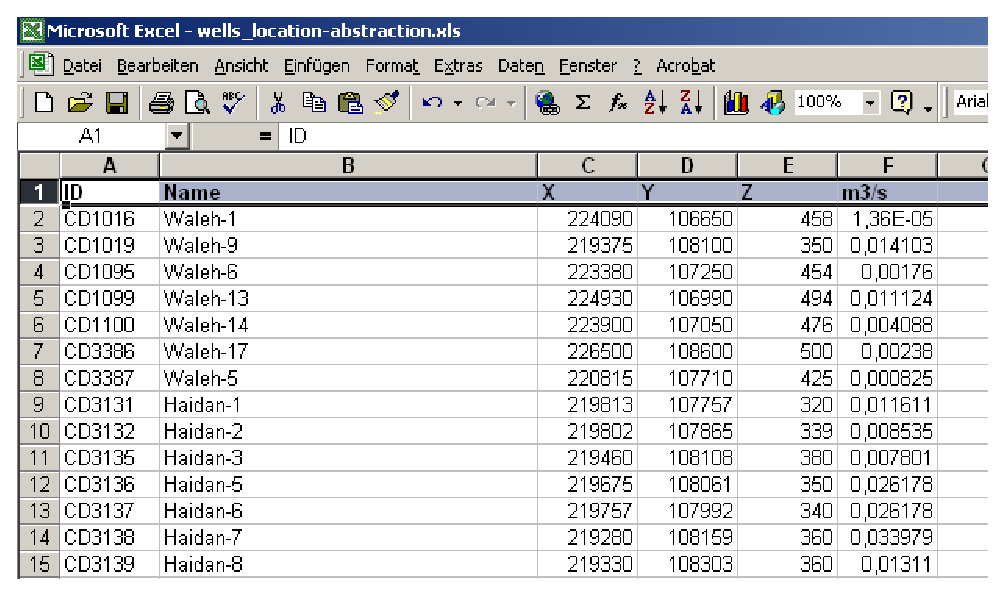
\includegraphics[width=12cm]{figures/st_data_base.eps}\\
  \caption{EXCEL sheet for well data import}
  \label{fig:st_excel}
\end{figure}

\subsubsection{Analytical source term}
This is an example for a fracture plane in a rock body. Here the
solution is applied to two processes, heat transport and mass
transport. The \$PCS\_TYPE defines the process for which the
source term is to be applied. The \$GEO\_TYPE specifies DOMAIN
indicating all nodes in the specified material group (value 1) act
as sources.

\begin{verbatim}
benchmark: frac_an.st
#SOURCE_TERM
 $PCS_TYPE
  MASS_TRANSPORT
 $PRIMARY_VARIABLE
  CONCENTRATION1
 $GEO_TYPE
  DOMAIN
 $DIS_TYPE
  ANALYTICAL 0 1.e-6 50

#SOURCE_TERM
 $PCS_TYPE
  HEAT_TRANSPORT
 $PRIMARY_VARIABLE
  TEMPERATURE1
 $GEO_TYPE
  DOMAIN
 $DIS_TYPE
  ANALYTICAL 0 1.e-3 50
\end{verbatim}

Three variables are required

value 1: material group of the fracture

value 2: diffusion constant in matrix

value 3: number of previous time steps to be taken into account
(max 50).

The method will be documented in a forthcoming publication. It is
currently only available for triangular and quadratic elements
acting as 2D elements in 3D space, here representing fractures in
matrix.

\LastModified{CMCD - 19th December 2005}

%------------------------------------------
% OUT - Output
\section{Data Output}
\label{sec:out}

\begin{tabular*}{8.35cm}{|p{2.5cm}|p{5cm}|} \hline
Object acronym & OUT \\
C++ class      & COutput \\
Source files   & rf\_out.h/cpp \\
\hline
File extension & *.out \\
Object keyword & \#OUTPUT \\
\hline
\end{tabular*}

Three types of data output are
available:
\begin{itemize}
    \item VAR\_TYPE: Output for variables (primary and secondary).
    If no PCS\_TYPE and no MSH\_TYPE are specified, all PCS are
    screened for the given variables (standard case).
    \item PCS\_TYPE: Output for processes. Output only for the
    given PCS.
    \item MSH\_TYPE: Output for meshes. Output only for the given
    MSH.
\end{itemize}

%-------------------------------------------------------------------------------
\subsection{\texttt{\bf\#OUTPUT}}

%\subsubsection{Keyword structure}

\begin{verbatim}
#VERSION       //Given:  show version in all output file names
#OUTPUT
 $PCS_TYPE // physical process
  LIQUID_FLOW       // H process (incompressible flow)
  UNCONFINED_FLOW   // H process (incompressible flow)
  GAS_FLOW          // H process (compressible flow)
  TWO_PHASE_FLOW    // H2 process (incompressible/compressible flow)
  COMPONENTAL_FLOW  // H2 process (incompressible/compressible flow)
  RIVER_FLOW        // H process (incompressible flow)
  RICHARDS_FLOW     // H process (incompressible flow)
  OVERLAND_FLOW     // H process (incompressible flow)
  HEAT_TRANSPORT    // T process (single/multi-phase flow)
  DEFORMATION       // M process (single/multi-phase flow)
  MASS_TRANSPORT    // C process (single/multi-phase flow)
  GROUNDWATER_FLOW  // H process (incompressible flow)
  FLUID_MOMENTUM
 $MSH_TYPE // mesh
  msh_name //4.2.14(OK)
 $NOD_VALUES // specified node quantities
  PRESSUREx
  SATURATIONx
  TEMPERATURE1
  DISPLACEMENT1_X
  DISPLACEMENT1_Y
  DISPLACEMENT1_Z
  CONCENTRATION1
  CONCENTRATIONx
  STRESS_XX
  STRESS_XY
  STRESS_YY
  STRESS_ZZ
  STRESS_XZ
  STRESS_YZ
  STRAIN_XX
  STRAIN_XY
  STRAIN_YY
  STRAIN_ZZ
  STRAIN_XZ
  STRAIN_YZ
  STRAIN_PLS
  VELOCITY1_X
  VELOCITY1_Y
  VELOCITY1_Z
 $ELE_VALUES // specified element quantities
  VELOCITY1_X
  VELOCITY1_Y
  VELOCITY1_Z
  MASS_FLUX1_X
  MASS_FLUX1_Y
  MASS_FLUX1_Z
 $GEO_TYPE // geometry
  POINT    name
  POLYLINE name
  SURFACE  name
  VOLUME   name
  DOMAIN
  LAYER //4.3.20
 $TIM_TYPE // output times
  time1
  ...
  timex
 $DAT_TYPE // output file format
  TECPLOT
  ROCKFLOW // 4.2.14(OK)
  VTK      // 4.3.XX (GK)
 $DIS_TYPE // 4.2.14(OK)
  AVERAGE
 $AMPLIFIER // to amplify output data
  scale
#STOP
\end{verbatim}

In the case of  axisymmetrical deformation problem, the output of
stresses, strains and displacements have the following meanings:
\begin{gather}
   \stress_{xx}=\stress_{rr}, \quad  \stress_{yy}=\stress_{\theta\theta},\quad
  \stress_{zz}=\stress_{zz}, \stress_{xy}=\stress_{rz} \nonumber\\
   \strain_{xx}=\strain_{rr}, \quad  \strain_{yy}=\strain_{\theta\theta},\quad
  \strain_{zz}=\strain_{zz}, \strain_{xy}=\strain_{rz} \nonumber\\
  u_{x}=u_{r},\quad u_z=u_z \nonumber
\end{gather}

\begin{tabular*}{12.773cm}{|p{3.cm}|p{1.5cm}|p{7cm}|} \hline
Subkeyword          & Acronym & Meaning \\ \hline \hline
%
\texttt{PCS\_TYPE}   & PCS &  Specified process for output \\
\texttt{MSH\_TYPE}   & MSH &  Specified mesh for output \\
\texttt{NOD\_VALUES} & NOD &  Specified node values for output \\
\texttt{ELE\_VALUES} & ELE &  Specified element values for output \\
\texttt{GEO\_TYPE}   & GEO &  Related geometric objects \\
\texttt{TIM\_TYPE}   & TIM &  Specified output times \\
\texttt{DAT\_TYPE}   & DAT &  Output file format \\
\texttt{DIS\_TYPE}   & DIS &  Output methods (e.g. averaging) \\
\hline
\end{tabular*}

\subsubsection{\texttt{\$PCS\_TYPE}}

see section \ref{sec:pcs}.

\subsubsection{\texttt{\$MSH\_TYPE}}

see section \ref{sec:msh}.

\subsubsection{\texttt{\$NOD\_VALUES}}

see section \ref{sec:nod_values}

\subsubsection{\texttt{\$GEO\_TYPE}}

see section \ref{sec:geo_types}

%OK
\small
\begin{verbatim}
LAYER //4.3.20
\end{verbatim}
\normalsize \vspace{-2mm}
%
This specification produces layer output for regional processes
(e.g. regional soil model).

\subsubsection{\texttt{\$TIM\_TYPE}}

\begin{tabular*}{12.773cm}{|p{3.cm}|p{8.9cm}|} \hline
Parameter        & Meaning \\ \hline \hline
%
\texttt{...}     & List of output times \\
\texttt{STEPS}   & Interval of output steps \\
\hline
\end{tabular*}

\subsubsection{\texttt{\$DAT\_TYPE}}

\begin{tabular*}{12.773cm}{|p{3.cm}|p{8.9cm}|} \hline
Parameter        & Meaning \\ \hline \hline
%
\texttt{TECPLOT}  & Tecplot file format (tec file) \\
\texttt{ROCKFLOW} & RockFlow file format (rfo file) \\
\texttt{VTK} & Paraview file format (vtk file) \\
\hline
\end{tabular*}

\subsubsection{\texttt{\$DIS\_TYPE}}

\begin{tabular*}{12.773cm}{|p{3.cm}|p{8.9cm}|} \hline
Parameter        & Meaning \\ \hline \hline
%
\texttt{AVERAGE} & nodal average \\
\hline
\end{tabular*}


\Examples{
%===============================================================================
\subsection{Examples}

%-------------------------------------------------------------------------------
\subsubsection{VAR\_TYPE: Output for variables}

%...............................................................................
\subsubsection*{Output files}

The names of the OUT files are generated automatically:

\begin{tabular*}{12.773cm}{|p{3.cm}|p{8.9cm}|} \hline
Parameter          & File name \\ \hline \hline
%
Domain      & node values: \texttt{filename\_dom\_nod.tec} \\
Domain      & element values: \texttt{filename\_dom\_ele.tec} \\
Time curves & \texttt{filename\_time\_GEOName.tec} \\
Profiles    & \texttt{filename\_GEOName\_TIMStepNumber.tec} \\
\hline
\end{tabular*}

%...............................................................................
\subsubsection*{Domain output}

Data output of \texttt{PRESSURE1} at $t$ = 4.320000e+003 sec for
whole domain.

\begin{verbatim}
benchmark: h_tet3.out
#OUTPUT // domain
 $NOD_VALUES
  PRESSURE1
 $GEO_TYPE
  DOMAIN
 $DAT_TYPE
  TECPLOT
 $TIM_TYPE
  4.320000e+003
#STOP
\end{verbatim}

Data output of \texttt{PRESSURE1} each time step for whole domain.

\begin{verbatim}
#OUTPUT // domain
 $NOD_VALUES
  PRESSURE1
 $GEO_TYPE
  DOMAIN
 $DAT_TYPE
  TECPLOT
 $TIM_TYPE
  STEPS 1
#STOP
\end{verbatim}

%...............................................................................
\subsubsection{Time curve output}

Data output of \texttt{PRESSURE1} and \texttt{TEMPERATURE1} in
\texttt{POINT2} for all time steps.

\begin{verbatim}
benchmark: ht_line.out
#OUTPUT // time curve
 $NOD_VALUES
  PRESSURE1
  TEMPERATURE1
 $GEO_TYPE
  POINT POINT2
 $DAT_TYPE
  TECPLOT
#STOP
\end{verbatim}

Data output of node average at surface \texttt{OUT} for all time steps.

\begin{verbatim}
benchmark: h2_line.out
#OUTPUT // profile
 $NOD_VALUES
  CONCENTRATION
 $GEO_TYPE
  SURFACE OUT
 $TIM_TYPE
  STEPS 1
 $DIS_TYPE
  AVERAGE
#STOP
\end{verbatim}

%...............................................................................
\subsubsection{Profile output}

Data output of \texttt{PRESSURE1} and \texttt{SATURATION2} along
polyline \texttt{OUT} at times $t$ = 5e+5, 1e+6, 5e+6, 1e+7, 5e+7,
1e+8 and 2e+8 sec.

\begin{verbatim}
benchmark: h2_line.out
#OUTPUT // profile
 $NOD_VALUES
  PRESSURE1
  SATURATION2
 $GEO_TYPE
  POLYLINE OUT
 $DAT_TYPE
  TECPLOT
 $TIM_TYPE
  5e+5
  1e+6
  5e+6
  1e+7
  5e+7
  1e+8
  2e+8
#STOP
\end{verbatim}

%-------------------------------------------------------------------------------
\subsubsection{MSH\_TYPE: Output for meshes}

%...............................................................................
\subsubsection*{Output files}

The names of the OUT files are generated automatically:

\begin{tabular*}{12.773cm}{|p{3.cm}|p{8.9cm}|} \hline
Parameter          & File name \\ \hline \hline
%
Domain      & node values: \texttt{filename\_dom\_MSHName\_nod.tec} \\
Domain      & element values: \texttt{filename\_dom\_MSHName\_ele.tec} \\
Time curves & \texttt{filename\_time\_MSHName\_GEOName.tec} \\
Profiles    & \texttt{filename\_MSHName\_GEOName\_TIMStepNumber.tec} \\
\hline
\end{tabular*}

Output for two meshes (regional soil model).

\begin{verbatim}
benchmark: 2.out
#OUTPUT
 $MSH_TYPE
  SURFACE0
 $NOD_VALUES
  PRESSURE1
  SATURATION1
 ...
#OUTPUT
 $MSH_TYPE
  SURFACE1
 $NOD_VALUES
  PRESSURE1
  SATURATION1
 ...
#STOP
\end{verbatim}


%-------------------------------------------------------------------------------
\subsubsection{PCS\_TYPE: Output for meshes}

%...............................................................................
\subsubsection*{Output files}

The names of the OUT files are generated automatically:

\begin{tabular*}{12.773cm}{|p{3.cm}|p{8.9cm}|} \hline
Parameter          & File name \\ \hline \hline
%
Domain      & node values: \texttt{filename\_dom\_PCSName\_nod.tec} \\
Domain      & element values: \texttt{filename\_dom\_PCSName\_ele.tec} \\
Time curves & \texttt{filename\_time\_PCSName\_GEOName.tec} \\
Profiles    & \texttt{filename\_PCSName\_GEOName\_TIMStepNumber.tec} \\
\hline
\end{tabular*}


}

\LastModified{OK - 30.12.2005}

%------------------------------------------
% TIM - Time discretization
\section{Time Discretization}

\begin{tabular*}{8.35cm}{|p{2.5cm}|p{5cm}|} \hline
Object acronym & TIM \\
C++ class      & CTimeDiscretization \\
Source files   & rf\_tim.h/cpp \\
\hline
File extension & *.tim \\
Object keyword & \#TIME\_STEPPING \\
\hline
\end{tabular*}

\Developer{
%----------------------------------------------------------
\subsection{Theory}
}

%-------------------------------------------------------------------------------
\subsection{\texttt{\bf\#TIME\_STEPPING}}

%\subsubsection{Keyword structure}

\begin{verbatim}
#TIME_STEPPING
 $PCS_TYPE // physical process
  LIQUID_FLOW       // H process (incompressible flow)
  UNCONFINED_FLOW   // H process (incompressible flow)
  RICHARDS_FLOW     // H process (incompressible flow)
  GAS_FLOW          // H process (compressible flow)
  TWO_PHASE_FLOW    // H2 process (incompressible/compressible flow)
  COMPONENTAL_FLOW  // H2 process (incompressible/compressible flow)
  RIVER_FLOW        // H process (incompressible flow)
  OVERLAND_FLOW     // H process (incompressible flow)
  HEAT_TRANSPORT    // T process (single/multi-phase flow)
  DEFORMATION       // M process (single/multi-phase flow)
  MASS_TRANSPORT    // C process (single/multi-phase flow)
  GROUNDWATER_FLOW  // H process (incompressible flow)
 $TIME_STEPS
  no_steps time_step_length
  ...
 $TIME_UNIT
  SECOND
  HOUR
  DAY
  YEAR
 $TIME_END
  time_end
 $TIME_START
  time_start
 $TIME_CONTROL
  COURANT
  NEUMANN           // Only available for Richards flow
  PECLET
  SELF_ADAPTIVE
  ERROR_CONTROL_ADAPTIVE     // Only available for Richards flow
 #STOP
\end{verbatim}


\begin{tabular*}{12.773cm}{|p{3.cm}|p{1.5cm}|p{7cm}|} \hline
Subkeyword             & Data type & Meaning \\ \hline \hline
%
\texttt{PCS\_TYPE}     & string     &  Specified processes for time stepping \\
\texttt{TIME\_STEPS}   & int,double &  Number of time steps and time step length \\
\texttt{TIME\_UNIT}    & string     &  Unit of time step, default value is second \\
\texttt{TIME\_START}   & double     &  Start time \\
\texttt{TIME\_END}     & double     &  End time \\
\texttt{TIME\_CONTROL} & string     &  Criterion for time step control \\
\hline
\end{tabular*}

\subsubsection{\texttt{\$PCS\_TYPE}}

\begin{tabular*}{10.853cm}{|p{3.cm}|p{7cm}|} \hline
Parameter          &Meaning \\ \hline \hline
%
\texttt{FLUID\_FLOW}     &Time stepping for flow process \\
\texttt{HEAT\_TRANSPORT} &Time stepping for heat transport process \\
\texttt{DEFORMATION}     &Time stepping for deformation process \\
\texttt{MASS\_TRANSPORT} &Time stepping for mass transport process \\
\texttt{RIVER\_FLOW}     &Time stepping for river flow process \\
\texttt{RICHARDS\_FLOW}     &Time stepping for Richards flow process \\
\hline
\end{tabular*}

\Examples{
\newpage
%-------------------------------------------------------------------------------
\subsection{Examples}

%-------------------------------------------------------------------------------
\subsubsection{Domain output}

Data output of \texttt{PRESSURE1} at $t$ = 4.320000e+003 sec for
whole domain.

\begin{verbatim}
benchmark: th2_line.tim
#TIME_STEPPING
 $PCS_TYPE
  LIQUID_FLOW
 $TIME_STEPS
 1000  1e+0
 100  1e+1
 100  2e+1
 400  5e+1
 $TIME_START
  0.0
 $TIME_END
  2.e+4
#STOP
\end{verbatim}

\begin{verbatim}
benchmark: h_us_line_warrick.tim
#TIME_STEPPING
 $PCS_TYPE
  RICHARDS_FLOW
 $TIME_END
  61200.0
 $TIME_START
  0.0
 $TIME_CONTROL
  NEUMANN
#STOP
\end{verbatim}

\begin{verbatim}
benchmark: h_us_line_forsyth.tim
#TIME_STEPPING
 $PCS_TYPE
  RICHARDS_FLOW
 $TIME_UNIT
  HOUR
 $TIME_END
  240
 $TIME_START
  0.0
 $TIME_CONTROL
   SELF-ADAPTIVE
   4    1.7
   10   0.7
   MAX_TIME_STEP
   1
   MIN_TIME_STEP
   0.00001
#STOP
\end{verbatim}

\begin{verbatim}
benchmark: h_us_line_warrick.tim #TIME_STEPPING
 $PCS_TYPE
  RICHARDS_FLOW
 $TIME_END
  61200.0
 $TIME_START
  0.0
 $TIME_CONTROL
  ERROR_CONTROL_ADAPTIVE
#STOP
\end{verbatim}

}

\LastModified{YD - \today}

%------------------------------------------
% MFP - Fluid properties
\section{Fluid Properties}

\begin{tabular*}{8.35cm}{|p{2.5cm}|p{5cm}|} \hline
Object acronym & MFP \\
C++ class      & CFluidProperties \\
Source files   & rf\_mfp.h/cpp \\
\hline
File extension & *.mfp \\
Object keyword & \#FLUID\_PROPERTIES \\
\hline
\end{tabular*}

%-------------------------------------------------------------------------------
\subsection{\texttt{\bf\#FLUID\_PROPERTIES}}

%\subsubsection{Keyword structure}

\begin{verbatim}
#FLUID_PROPERTIES
 $FLUID_TYPE
  AIR
 $DENSITY
  model model_parameters
 $VISCOSITY
  model model_parameters
 $SPECIFIC_HEAT_CAPACITY
  model model_parameters
 $HEAT_CONDUCTIVITY
  model model_parameters
 $PHASE_DIFFUSION
  model model_parameters
 $NON_GRAVITY
  model model_parameters
\end{verbatim}

\begin{itemize}
  \item fluid type for data base operation
  \item model / model parameters
\end{itemize}


%==========================================================
\subsection{Fluid model data input}

\begin{itemize}
  \item organized by flow types
\end{itemize}

%----------------------------------------------------------
\subsubsection{Fluid density}

%-------------------------------------------------------------------------------
\paragraph*{Case 0: User-defined function by \#CURVE}
\begin{eqnarray}
  \Density^\Phase= f(u)
\end{eqnarray}
\begin{verbatim}
$DENSITY
 0 curve_number
\end{verbatim}

\paragraph*{Case 1: Incompressible flow}
\begin{eqnarray}
  \Density^\Phase = \Density^\Phase_0
\end{eqnarray}
\begin{verbatim}
$DENSITY
 1 rho_0
\end{verbatim}

\paragraph*{Case 2: Compressible flow}
\begin{eqnarray}
  \Density^\Phase(\Pressure)
  = \Density_0^\Phase(1+\FluidCompressibility^\Phase(\Pressure^\Phase-\Pressure^\Phase_0))
\end{eqnarray}
\begin{verbatim}
$DENSITY
 2  rho_0  beta_p  p_0
\end{verbatim}

\paragraph*{Case 3: Density-dependent flow, mass convection}
\begin{eqnarray}
  \Density^\Phase(\Conc)
  = \Density_0^\Phase(1+\beta_C^\Phase(\Conc-\Conc_0))
\end{eqnarray}
\begin{verbatim}
$DENSITY
 3  rho_0  beta_C  C_0
\end{verbatim}

\paragraph*{Case 4: Density-dependent flow, thermal convection}
\begin{eqnarray}
  \Density^\Phase(\Temperature)
  = \Density_0^\Phase(1+\ThermalExpansionCoefficient^\Phase(\Temperature-\Temperature_0))
\end{eqnarray}
\begin{verbatim}
$DENSITY
 4  rho_0  beta_T  T_0
\end{verbatim}

\paragraph*{Case 5: Density-dependent flow, thermohalin convection}
\begin{eqnarray}
  \Density^\Phase(\Conc,\Temperature)
  = \Density_0^\Phase(1+\beta_C^\Phase(\Conc-\Conc_0)
  + \Density_0^\Phase(1+\ThermalExpansionCoefficient^\Phase(\Temperature-\Temperature_0))
\end{eqnarray}
\begin{verbatim}
$DENSITY
 5  rho_0  beta_C  C_0  beta_T  T_0
\end{verbatim}

\paragraph*{Case 6: Compressible non-isothermal flow}
\begin{eqnarray}
  \Density^\Phase(\Pressure,\Temperature)
  = \Density_0^\Phase(1+\FluidCompressibility^\Phase(\Pressure^\Phase-\Pressure^\Phase_0)
  + \Density_0^\Phase(1+\ThermalExpansionCoefficient^\Phase(\Temperature-\Temperature_0))
\end{eqnarray}
\begin{verbatim}
$DENSITY
 6  rho_0  beta_p  p_0  beta_T  T_0
\end{verbatim}

\paragraph*{Case 7: Compressible non-isothermal flow with phase changes}
\begin{eqnarray}
  \Density^g(\Pressure^g,\Temperature)=
  \frac{\MolarMass_a}{\GasConstant\Temperature}\Pressure^g+\frac{(\MolarMass_w -
  \MolarMass_a)}{\GasConstant\Temperature}\VapourPressure(\Temperature)
\end{eqnarray}
\begin{verbatim}
$DENSITY
 7
\end{verbatim}


%----------------------------------------------------------
\subsubsection{Fluid viscosity}
%-------------------------------------------------------------------------------
\paragraph*{Case 0: User-defined function by \#CURVE}
\begin{eqnarray}
\Viscosity^\Phase= f(u)
\end{eqnarray}
\begin{verbatim}
$VISCOSITY
 0  curve_number
\end{verbatim}

\paragraph*{Case 1: Incompressible flow}
\begin{eqnarray}
\Viscosity^\Phase(\Pressure) = \Viscosity_0^\Phase
\end{eqnarray}
\begin{verbatim}
$VISCOSITY
 1  my_0
\end{verbatim}

\paragraph*{Case 2: Compressible flow}
\begin{eqnarray}
\Viscosity^\Phase(\Pressure)
=
\Viscosity_0^\Phase \left(1 + \frac{d\Viscosity}{d\Pressure} (p-p_0)\right)
\end{eqnarray}
\begin{verbatim}
$VISCOSITY
 2  my_0  dmy_dp  p_0
\end{verbatim}

\paragraph*{Case 3: Density-dependent flow, mass convection}
\begin{eqnarray}
\Viscosity^\Phase(\Conc,\Temperature)
=
\frac{\Viscosity}{f1 + f2}
\quad
f1= f(\Conc), f2=f(\Temperature)
\end{eqnarray}
\begin{verbatim}
$VISCOSITY
 3  my_0  dmy_dC  0.0
\end{verbatim}

\paragraph*{Case 4: Density-dependent flow, thermal convection}
\begin{eqnarray}
\Viscosity^\Phase(\Conc,\Temperature)
=
\frac{\Viscosity}{f1 + f2}
\quad
f1= f(\Conc), f2=f(\Temperature)
\end{eqnarray}
\begin{verbatim}
$VISCOSITY
 4  my_0  0.0  dmy_dT
\end{verbatim}

\paragraph*{Case 41: Non-isothermal liquid flow (Yaws et al. 1976)}
\begin{eqnarray}
\Viscosity^l(\Temperature)
=
10^{-3} \exp(-2.471 10^1+\frac{4.209 10^3}{\Temperature}
+
4.527 10^{-2}\Temperature-3.376 10^{-5}\Temperature^2)
\end{eqnarray}
\begin{verbatim}
$VISCOSITY
 41
\end{verbatim}

\paragraph*{Case 5: Density-dependent flow, thermohaline convection}
\begin{eqnarray}
\Viscosity^\Phase(\Conc,\Temperature)
=
\frac{\Viscosity}{f1 + f2}
\quad
f1= f(\Conc), f2=f(\Temperature)
\end{eqnarray}
\begin{verbatim}
$VISCOSITY
 5  my_0  dmy_dC  dmy_dT
\end{verbatim}

\paragraph*{Case 6: Compressible non-isothermal flow (Reichenberg 1971)}
\begin{eqnarray}
\Viscosity^\Phase(\Pressure,\Temperature)
=
\Viscosity_0 [1+ \frac{A(\frac{\Pressure}{33.9
10^4})^{1.5}}{B(\frac{\Pressure}{33.9 10^4}) +
\frac{1}{C(\frac{\Pressure}{33.9 10^4})^D}}]
\end{eqnarray}
\begin{verbatim}
$VISCOSITY
 6
\end{verbatim}

\paragraph*{Case 61: Non-isothermal gas flow (Marsily 1986)}
\begin{eqnarray}
\Viscosity^g(\Temperature)
=
2.285\cdot10^{-5} + 1.01 \cdot10^{-3}\log{T}
\end{eqnarray}
\begin{verbatim}
$VISCOSITY
 61
\end{verbatim}

\paragraph*{Case 7: Compressible non-isothermal flow with phase changes (Reichenberg 1971)}
\begin{eqnarray}
\Viscosity^\Phase(\Pressure,\Temperature)
=
\Viscosity_0 [1+ \frac{A(\frac{\Pressure}{33.9
10^4})^{1.5}}{B(\frac{\Pressure}{33.9 10^4}) +
\frac{1}{C(\frac{\Pressure}{33.9 10^4})^D}}]
\end{eqnarray}
\begin{verbatim}
$VISCOSITY
 7
\end{verbatim}

%----------------------------------------------------------
\subsubsection{Specific heat capacity}

%-------------------------------------------------------------------------------
\paragraph*{Case 0: User-defined function by \#CURVE}
\begin{eqnarray}
  \HeatCapacity^\Phase= f(\Temperature)
\end{eqnarray}
\begin{verbatim}
$SPECIFIC_HEAT_CAPACITY
 0 curve_number
\end{verbatim}

\paragraph*{Case 1: Constant}
\begin{eqnarray}
  \HeatCapacity^\Phase = \HeatCapacity^\Phase_0
\end{eqnarray}
\begin{verbatim}
$SPECIFIC_HEAT_CAPACITY
 1 rho_0
\end{verbatim}

\paragraph*{Case 2: Simple enthalpy based phase change}
\begin{eqnarray}
  \HeatCapacity^\Phase
  = f(\Enthalpy,\Temperature)
\end{eqnarray}
\begin{eqnarray}
  \Enthalpy^\Phase
  = f(\HeatCapacity,\Temperature)
\end{eqnarray}
\begin{verbatim}
$SPECIFIC_HEAT_CAPACITY
 2
\end{verbatim}

\paragraph*{Case 3: Phase change, enthalpy defined by \#CURVE}
\begin{eqnarray}
  \HeatCapacity^\Phase
  = f(\Enthalpy,\Temperature)
\end{eqnarray}
\begin{eqnarray}
  \Enthalpy^\Phase
  = f(\Temperature)
\end{eqnarray}
\begin{verbatim}
$SPECIFIC_HEAT_CAPACITY
 3  T_latent1  T_latent1 curve number
\end{verbatim}

\paragraph*{Case 4: LBNL Phase change model}
\begin{eqnarray}
 \HeatCapacity =
(1-n)\rho^sc^s+nS^l\rho^lc^l+nS^g\rho^gc^g+H_1\bigg(e^{\frac{p^l}{\rho^l}R\Temperature}\frac{\partial
\rho_s^g}{\partial
\Temperature}-\frac{\rho^gp^l}{R\Temperature^2}\bigg)
\end{eqnarray}\\

\begin{eqnarray}
H_1=nS^g(L_0+c^g(\Temperature-\TLatentB))
\end{eqnarray}\\
\begin{verbatim}
$SPECIFIC_HEAT_CAPACITY
 4  T_latent1  T_latent1 Latent_heat
\end{verbatim}

%-------------------------------------------------------------------------------
\subsubsection*{Nomenclature}
\begin{tabular}{ll}
$\Conc$ & concentration\\
$\HeatCapacity $ & specific heat capacity\\
$\Enthalpy$ & enthalpy\\
$\MolarMass_a$ & molar mass of air\\
$\MolarMass_w$ & molar mass of water\\
$\LatentHeat$ & Latent heat\\
$\Pressure$ & pressure\\
$\VapourPressure$ & saturated vapor pressure\\
$\GasConstant$ & ideal gas constant\\
$\Temperature$ & temperature\\
$\TLatentB$ & temperature of beginning phase change\\
$\TLatentE$ & temperature of ending phase change\\
$\beta_C$ & solutal expansion coefficient\\
$\FluidCompressibility$ & compressibility\\
$\ThermalExpansionCoefficient$ & thermal expansion coefficient\\
$\Phase$ & phase\\
$\Viscosity$ & viscosity\\
$\Density$ & density\\
subscript 0 &  reference value\\
\end{tabular}



\newpage
\Examples{
%-------------------------------------------------------------------------------
\subsection{Examples}

%-------------------------------------------------------------------------------
\subsubsection{Single phase flow}

\begin{verbatim}
benchmark: h_line.mfp
#FLUID_PROPERTIES
 $FLUID_TYPE
  LIQUID
 $PCS_TYPE
  PRESSURE1
 $DENSITY
  1 1.000000e+003
 $VISCOSITY
  1 1.000000e-003
#STOP
\end{verbatim}

%-------------------------------------------------------------------------------
\subsubsection{Two phase flow}

\begin{verbatim}
benchmark: h2_line.mfp
#FLUID_PROPERTIES
 $FLUID_TYPE
  LIQUID
 $PCS_TYPE
  PRESSURE1
 $DENSITY
  1 1.000000e+003
 $VISCOSITY
  1 1.000000e-003
#FLUID_PROPERTIES
 $FLUID_TYPE
  LIQUID
 $PCS_TYPE
  SATURATION2
 $DENSITY
  1 1.000000e+003
 $VISCOSITY
  1 1.000000e-003
#STOP
\end{verbatim}

%-------------------------------------------------------------------------------
\subsubsection{Non-isothermal two phase flow}

\begin{verbatim}
benchmark: th2_line.mfp
#FLUID_PROPERTIES // first fluid phase
 $FLUID_TYPE
  GAS
 $PCS_TYPE
  PRESSURE1
 $DENSITY
  2 1.26 1.e5 6.6667e-6
 $VISCOSITY
  1 1.8e-5
 $HEAT_CAPACITY
  1 1.01e+3
 $HEAT_CONDUCTIVITY
  1 0.026
 $PHASE_DIFFUSION
  1 2.13e-6
#FLUID_PROPERTIES // second fluid phase
 $FLUID_TYPE
  LIQUID
 $PCS_TYPE
  SATURATION2
 $DENSITY
  2 1000. 1.e5 4.7e-7
 $VISCOSITY
  1 0.0012
 $HEAT_CAPACITY
  1 4200.
 $HEAT_CONDUCTIVITY
  1 0.6
 $PHASE_DIFFUSION
  1 2.13e-6
#STOP
\end{verbatim}

%-------------------------------------------------------------------------------
\subsubsection{Consolidation}

\begin{verbatim}
benchmark: hm_tri.mfp
#FLUID_PROPERTIES
 $FLUID_TYPE
  LIQUID
 $PCS_TYPE
  PRESSURE1
 $DENSITY
  1 0.0
 $VISCOSITY
  1 1.000000e-003
#STOP
\end{verbatim}

%-------------------------------------------------------------------------------
\subsubsection{Heat transport}

\begin{verbatim}
benchmark: ht_line.mfp
#FLUID_PROPERTIES
 $FLUID_TYPE
  LIQUID
 $PCS_TYPE
  PRESSURE1
 $DENSITY
  1 1.000000e+003
 $VISCOSITY
  1 1.000000e-003
 $HEAT_CAPACITY
  1 4.280000e+003
 $HEAT_CONDUCTIVITY
  1 6.000000e-001
#STOP
\end{verbatim}

} % Examples

\LastModified{YD - \today}

%------------------------------------------
% MSP - Solid properties
\section{Solid Properties}

\begin{tabular*}{8.35cm}{|p{2.5cm}|p{5cm}|} \hline
Object acronym & MSP \\
C++ class      & CSolidProperties \\
Source files   & rf\_msp.h/cpp \\
\hline
File extension & *.msp \\
Object keyword & \#SOLID\_PROPERTIES \\
\hline
\end{tabular*}

\Developer{
%----------------------------------------------------------
\subsection{Theory}
}

%-------------------------------------------------------------------------------
\subsection{\texttt{\bf\#SOLID\_PROPERTIES}}

%\subsubsection{Keyword structure}

\begin{verbatim}
#SOLID_PROPERTIES
// Data base
 $SOLID_TYPE
  BENTONITE
  CLAY
// Mechanical properties
 $DENSITY
  model model_parameters
 $ELASTICITY
  poisson_model model_parameters
  elasticity_model model_parameters
 $PLASTICITY
  model_name model_parameters
 $VISCOSITY
  model model_parameters
// Thermal properties
 $HEAT_CAPACITY
  model model_parameters
 $HEAT_CONDUCTIVITY
  model model_parameters
 $THERMAL_EXPANSION
  model model_parameters
...
#STOP
\end{verbatim}

\subsection{Heat capacity}
\begin{itemize}
  \item mode 0: User defined curve (not available)
  \item mode 1: Constant number
  \item mode 2: Boiling mode, medium property. Input format: [mode] [\mbox{wet capacity}]
                     [\mbox{dry capacity}]   [\mbox{boiling temperature}]
                     [\mbox{duration temperature}]  [\mbox{heat latent}]
 \item mode 3: Temperature and saturation dependent heat capacity, solid property.  (DECOVALEX IV)
\end{itemize}

\subsection{Heat conductivity}
\begin{itemize}
  \item mode 0: User defined curve (not available)
  \item mode 1: Constant number
  \item mode 2: Boiling mode, medium properties. Input format: [mode] [\mbox{wet conductivity}]
                     [\mbox{dry conductivity}]   [\mbox{boiling temperature}]
                     [\mbox{duration temperature}]
  \item mode 3: Temperature and saturation dependent heat conductivity, solid property. (DECOVALEX IV)
\end{itemize}



\Examples{
%-------------------------------------------------------------------------------
\subsection{Examples}

%-------------------------------------------------------------------------------
\subsubsection{Drucker-Prager elasto-plasticity}
\begin{verbatim}
benchmark: m_dp_tri.msp
#SOLID_PROPERTIES
 $ELASTICITY
  1 3.0000e-001 // Poisson ratio
 $PLASTICITY
  DRUCKER-PRAGER
  1.0e6
  -1.0e+6
  20.0
  5.0
#STOP
\end{verbatim}

%-------------------------------------------------------------------------------
\subsubsection{Cam-Clay elasto-plasticity}
\begin{verbatim}
benchmark: m_cc_tri_s.msp, m_cc_quad_s.msp,  hm_cc_tri_s.msp
 #SOLID_PROPERTIES
 $ELASTICITY
  1 3.0000e-001 // Poisson ratio
 $PLASTICITY
  CAM-CLAY
   1.0    // M
   0.045  // Virgin compression index
   0.016  // Internal frictional angle
   4.2e4  // Initial pre-consolidation pressure
   0.285  // Initial void ratio
   1.0    // OCR
   -0.9e4 // Initial stress_xx
   -2.1e4 // Initial stress_yy
   -0.9e4 // Initial stress_zz
   0.0    // Minimum (stress_xx+stress_yy+stress_zz). Only for some special cases
#STOP
\end{verbatim}

\subsubsection{Norton creep model}
\begin{verbatim}
benchmark: m_crp_tri.msp
#SOLID_PROPERTIES
  $DENSITY
  1 0.0
  $ELASTICITY
    POISSION  0.3
    YOUNGS_MODULUS
      1 100.0
  $CREEP_NORTON
    10e-10 5.0
#STOP
\end{verbatim}

%-------------------------------------------------------------------------------
\subsubsection{Single-Yield-Surface elasto-plasticity (Ehlers)}
\begin{verbatim}
benchmark: m_dp_tri.msp
#SOLID_PROPERTIES
 $ELASTICITY
  1 3.0000e-001 // Poisson ratio
  1 1.90139e+08 // Youngs modulus
 $PLASTICITY
  SINGLE-YIELD-SURFACE
   0.      // alpha0
   0.26    // beta0
   3.5e-7  // delta0
   1.0e-7  // epsilon0
   0.0     // kappa0
   0.0     // gamma0
   0.569   // m0
   0.      // alpha1
   0.29    // beta1
   8.81e-9 // delta1
   1.5e-8  // epsilon1
   0.      // kappa1
   0.0     // gamma1
   1.0     // m1
   0.55    // psi1
    -0.26  // psi2
   0.81e-3 // ch
   0.60e-3 // cd
   100.0   // br
   1.0     // mr
   0.0     // s_xx
   0.0     // s_yy
   0.0     // s_zz
#STOP
\end{verbatim}

\subsubsection{Discrete Fracture Deformation}
\begin{verbatim}
benchmark: frac_test.msp
#SOLID_PROPERTIES
  $ELASTICITY
    POISSION 1e-001
    YOUNGS_MODULUS:
     2 10.0e6 40.0e9 0.0006
#SOLID_PROPERTIES
  $ELASTICITY
    POISSION 1e-001
    YOUNGS_MODULUS:
     1 40.0e9
#STOP
\end{verbatim}
The two material groups represent the elastic properties of the fracture and matrix material. For the fracture, Young's modulus type 2 is defined. The value 10.0e6 is the modulus (in Pa) of the open fracture sections, the value 40.0e9 is the elastic modulus of closed fracture segments. The final parameter is the aperture (in m) below which the fracture is considered closed. The second material group defines the properties of the rock matrix, here it is defined as an elastic continuum with a constant Young's modulus of 40.0e9 Pa.

} % Examples

\LastModified{OK - \today}

%------------------------------------------
% MMP - Medium properties
\textcolor[rgb]{0.98,0.00,0.00}{\section{Porous Medium Properties}}

\begin{tabular*}{8.35cm}{|p{2.5cm}|p{5cm}|} \hline
Object acronym & MMP \\
C++ class      & CMediumProperties \\
Source files   & rf\_mmp.h/cpp \\
\hline
File extension & *.mmp \\
Object keyword & \#MEDIUM\_PROPERTIES \\
\hline
\end{tabular*}

\Developer{
%----------------------------------------------------------
\subsection{Theory}
}
%-------------------------------------------------------------------------------
\textcolor[rgb]{0.98,0.00,0.00}{\subsection{\texttt{\bf\#MEDIUM\_PROPERTIES - TORTUOSITY Changed}}}

%\subsubsection{Keyword structure}

\begin{verbatim}
#MEDIUM_PROPERTIES
// Data base
 $MEDIUM_TYPE
   CLAY
   SILT
   SAND
   GRAVEL
   CRYSTALLINE
// Geometric properties
 $GEOMETRY_DIMENSION
   dim // 1,2,3-D
 $GEOMETRY_AREA
   area // area for 1D element, thickness for 2D element
   FILE file.dat // input of distributed data (node or element wise)
 $GEO_TYPE
  POINT    point_name
  POLYLINE polyline_name
  SURFACE  surface_name
  VOLUME   volume_name
  LAYER    Layer_number
 $POROSITY
  model model_parameters
 $TORTUOSITY
  model model_parameters
  or
  ISOTROPIC   tortuosity
  ANISOTROPIC tortuosities
  FILE file_name
// Hydraulic properties
 $STORATIVITY
  model model_parameters
 $PERMEABILITY_TENSOR
  ISOTROPIC   permeability
  ORTHOTROPIC permeabilities
  ANISOTROPIC permeabilities
  FILE file_name
 $UNCONFINED
 $PERMEABILITY_FUNCTION_SATURATION
  model model_parameters for first fluid phase
  model model_parameters for second fluid phase
  ...
 $PERMEABILITY_FUNCTION_DEFORMATION
  model model_parameters
 $PERMEABILITY_FUNCTION_PRESSURE
  model model_parameters
 $PERMEABILITY_FUNCTION_STRESS
  model model_parameters
 $PERMEABILITY_FUNCTION_VELOCITY
  model model_parameters
 $PERMEABILITY_FRAC_APERTURE
  average_type roughness_correction
 $CAPILLARY_PRESSURE
  model model_parameters
 // Thermal properties
 $HEAT_DISPERSION
  model model_parameters
 // Mass transport properties
 $MASS_DISPERSION
  model model_parameters
 // Electric properties
 $ELECTRIC_CONDUCTIVITY
  model model_parameters
 // Multi-continua properties
 $FLUID_EXCHANGE
  model model_parameters
 $MASS_EXCHANGE
  model model_parameters
 $PERMEABILITY_DISTRIBUTION
  file_name
 $MANNING_COEFFICIENT
  value
 $FRACTURE_DATA
  number_of_fractures names_of_fractures
#STOP
\end{verbatim}

%==========================================================
\subsection{Medium model data input}
%----------------------------------------------------------
\subsubsection{Porosity}
\paragraph*{Case 11: Read in a file}
\begin{verbatim}
$POROSITY
 11 poro_layer1.dat
\end{verbatim}

%----------------------------------------------------------
%----------------------------------------------------------
\subsubsection{Friction coefficient for overland or channel flow}
\begin{verbatim}
$MANNING_COEFFICIENT
 0.15

$CHEZY_COEFFICIENT
 10
\end{verbatim}

%----------------------------------------------------------
%----------------------------------------------------------
\subsubsection{Permeability}
\paragraph*{PERMEABILITY\_TENSOR}
\begin{verbatim}
$PERMEABILITY_TENSOR
 FILE perm_layer1.dat
\end{verbatim}
%----------------------------------------------------------
%----------------------------------------------------------
\subsubsection{Discrete Fracture Permeability}
\begin{verbatim}
$PERMEABILITY_FRAC_APERTURE
  average_type roughness_correction
\end{verbatim}
\begin{itemize}
  \item average\_type: Arithmetic, Geometric, or Harmonic
  \item roughness\_correction: corr\_roughness OR no\_corr\_roughness
\end{itemize}
The average type describes how the average aperture (which is subsequently used to calculate the permeability) will be calculated. The permeability calculation is based on the cubic law. If $corr\_roughness$ is entered, this cubic law permeability will be corrected depending on the roughness of the fracture walls and the closure ratio of the fracture. This correction is based on:

Zimmerman RW, Bodvarsson GS (1996) Hydraulic Conductivity of Rock Fractures.
\emph{Transport in Porous Media} 23: 1-30

\emph{Note:} For this function to work polylines must be defined for the upper and lower fracture surface profiles. See \emph{frac\_test.gli}.

%----------------------------------------------------------
%----------------------------------------------------------
\subsubsection{Confined or unconfined flow}
Standard is the confined flow is modelled. No additional keyword
is required. If the mmp group is unconfined the keyword
\begin{verbatim}
$UNCONFINED
\end{verbatim}
has to be used.
%----------------------------------------------------------
%----------------------------------------------------------
\subsubsection{Relative permeability - saturation}
%----------------------------------------------------------


%-------------------------------------------------------------------------------
\paragraph*{Case 0: User-defined function by \#CURVE}
\begin{eqnarray}
  \PermRelS^\Phase= f(u)
\end{eqnarray}
\begin{verbatim}
$PERMEABILITY_SATURATION
 0 curve_number
\end{verbatim}

%-------------------------------------------------------------------------------
\paragraph*{Case 2: Linear function}

\paragraph*{Case 21: Linear function from saturation}
\begin{eqnarray}
\PermRelS^\Phase = 1-\Saturation^\Phase
\end{eqnarray}
\begin{verbatim}
$PERMEABILITY_SATURATION
 21
\end{verbatim}

%-------------------------------------------------------------------------------
\paragraph*{Case 4: van Genuchten (1980)}
\begin{eqnarray}
\SaturationEff
&=&
\frac{\Saturation^\Phase-\SaturationRes^\Phase}{\SaturationMax^\Phase-\SaturationRes^\Phase}
\\
\PermRelS^l &=& \SaturationEff^{1/2} \left[
1-(1-\SaturationEff^{1/m})^m \right]^2
\end{eqnarray}
\begin{verbatim}
$PERMEABILITY_SATURATION
 4  s_res  s_max  m
\end{verbatim}

%-------------------------------------------------------------------------------
\paragraph*{Case 14: van Genuchten 2 (1980)}
\begin{eqnarray}
\SaturationEff &=&
\frac{\Saturation^\Phase-\SaturationRes^\Phase}{\SaturationMax^\Phase-\SaturationRes^\Phase}
\\
\PermRelS^l &=& \SaturationEff^{0.5} \left[
1-(1-\SaturationEff^{1/m})^m \right]^2
\end{eqnarray}
\begin{verbatim}
$PERMEABILITY_SATURATION
 14  s_res  s_max  m
\end{verbatim}


%-------------------------------------------------------------------------------
\paragraph*{Case 14: van Genuchten (1980) for non-wettable phase}
\begin{eqnarray}
\SaturationEff &=&
\frac{\Saturation^\Phase-\SaturationRes^\Phase}{\SaturationMax^\Phase-\SaturationRes^\Phase}
\\
\PermRelS^g &=& (1-\SaturationEff)^{0.5} \left[
1-(1-\SaturationEff) \right]^{2m}
\end{eqnarray}
\begin{verbatim}
$PERMEABILITY_SATURATION
 15  s_res  s_max  m
\end{verbatim}

%----------------------------------------------------------
\subsubsection{Capillary pressure}

%-------------------------------------------------------------------------------
\textcolor[rgb]{0.98,0.00,0.00}{\paragraph*{Case 4: van Genuchten
(1980)}}
\begin{eqnarray}
p_c &=& \frac{\rho^lg}{\alpha}(\SaturationEff^{1/m}-1 )^{(1-m)}
\end{eqnarray}
\begin{verbatim}
 $CAPILLARY_PRESSURE
 4  alpha
 \end{verbatim}
%==========================================================
\Examples{
\newpage
%-------------------------------------------------------------------------------
%----------------------------------------------------------
\subsubsection{Discrete Fracture Data}
\begin{verbatim}
 $FRACTURE_DATA
  number_of_fractures names_of_fractures
\end{verbatim}
\begin{itemize}
  \item number\_of\_fractures: The number of discrete fractures in the model domain. Each fracture is handled as a separate entity.  
  \item names\_of\_fractures: The names of each of these fractures. For each fracture, polylines must be created representing the upper and lower fracture surface profiles. These polylines must have the names \emph{name\_of\_fracture\_top} and \emph{name\_of\_fracture\_bot}. See \emph{frac\_test.gli}.
\end{itemize}
%----------------------------------------------------------
\subsection{Examples}

%-------------------------------------------------------------------------------
\subsubsection{Single phase flow}

\begin{verbatim}
benchmark: h_line.mmp
#MEDIUM_PROPERTIES
 $GEOMETRY_DIMENSION
  1
 $GEOMETRY_AREA
  1.000000e+000
 $POROSITY
  1 2.000000e-001
 $TORTUOSITY
  1  1.000000e+000
 $PERMEABILITY_TENSOR
  ISOTROPIC 1.000000e-07
#STOP
\end{verbatim}


%-------------------------------------------------------------------------------
\subsubsection{Unconfined groundwater flow}

\begin{verbatim}
benchmark: beerze-reuzel.mmp
#MEDIUM_PROPERTIES
 $NAME
  Layer1
 $GEO_TYPE
  LAYER 1
 $GEOMETRY_DIMENSION
  2
 $GEOMETRY_AREA
  1.000000000000e+000
 $POROSITY
   11 sf1_1x.dat1
 $PERMEABILITY_TENSOR
   FILE   kd1_simgroq.dat1
 $UNCONFINED
\end{verbatim}

%-------------------------------------------------------------------------------
\subsubsection{Two phase flow}

\begin{verbatim}
benchmark: h2_line.mmp
#MEDIUM_PROPERTIES
 $GEOMETRY_DIMENSION
  1
 $GEOMETRY_AREA
  1.000000e+000
 $POROSITY
  1 2.000000e-001
 $TORTUOSITY
  1 1.000000e+000
 $PERMEABILITY_TENSOR
  ISOTROPIC 1.000000e-07
 $PERMEABILITY_SATURATION
  3 0.2 0.8 2.
  3 0.2 0.8 2.
 $CAPILLARY_PRESSURE
  0:
#STOP
\end{verbatim}

%-------------------------------------------------------------------------------
\subsubsection{Non-isothermal two phase flow}

\begin{verbatim}
benchmark: th2_line.mmp
#MEDIUM_PROPERTIES
 $GEOMETRY_DIMENSION
  1
 $GEOMETRY_AREA
  1.000000e-2
 $POROSITY
  1 0.407407407
 $TORTUOSITY
  1 0.8
 $PERMEABILITY_TENSOR
  ISOTROPIC: 8.22854E-20
 $PERMEABILITY_SATURATION
  21 0.0 0.9
  4  0.1 1.0 1.0
 $PERMEABILITY_DEFORMATION
  1 1.0 1.0 7.0 3293673.0 -0.165 3.0
 $CAPILLARY_PRESSURE
  0 5
#STOP
\end{verbatim}

%-------------------------------------------------------------------------------

\subsubsection{Richards flow}
\begin{verbatim}
benchmark: h_us_line.mmp #MEDIUM_PROPERTIES
 $GEOMETRY_DIMENSION
  3
 $GEOMETRY_AREA
  1.000000e+000
 $POROSITY
  1 2.000000e-001
 $TORTUOSITY
  1 1.000000e+000
 $PERMEABILITY_TENSOR
  ISOTROPIC 1.000000e-07
 $PERMEABILITY_SATURATION
  4  0  0.6452  0.791667
 $CAPILLARY_PRESSURE
  4  320
#STOP
\end{verbatim}

%-------------------------------------------------------------------------------
\subsubsection{Consolidation}

\begin{verbatim}
benchmark: hm_tri.mmp
#MEDIUM_PROPERTIES
 $GEOMETRY_DIMENSION
  2
 $GEOMETRY_AREA
  1.0
 $POROSITY
  1 0.000000e-001
 $TORTUOSITY
  1 1.000000e+000
 $PERMEABILITY_TENSOR
  ISOTROPIC 1.000000e-10
#STOP
\end{verbatim}

%-------------------------------------------------------------------------------
\subsubsection{Heat transport}

\begin{verbatim}
benchmark: ht_line.mmp
#MEDIUM_PROPERTIES
 $GEOMETRY_DIMENSION
  1
 $GEOMETRY_AREA
  1.0
 $POROSITY
  1 2.000000e-001
 $PERMEABILITY_TENSOR
  ISOTROPIC 1.000000e-11
 $HEAT_DISPERSION
  1 5.000000e+000 0.000000e+000
#STOP

\end{verbatim}

%-------------------------------------------------------------------------------
\subsubsection{Discrete Fracture Deformation}

\begin{verbatim}
benchmark: frac_test.mmp
#MEDIUM_PROPERTIES
 $GEOMETRY_DIMENSION
  2
 $GEOMETRY_AREA
  1.000000e+000
 $POROSITY
  1 1.000000e-001
 $TORTUOSITY
  1 1.000000e+000
 $PERMEABILITY_TENSOR
  ORTHOTROPIC 1 1
 $PERMEABILITY_FRAC_APERTURE
  Arithmetic corr_roughness
 $FRACTURE_DATA
  1 Frac0
#MEDIUM_PROPERTIES
 $GEOMETRY_DIMENSION
  2
 $GEOMETRY_AREA
  1.000000e+000
 $POROSITY
  1 1.000000e-005
 $TORTUOSITY
  1 1.000000e+000
 $PERMEABILITY_TENSOR
  ISOTROPIC 1.000000e-16
#STOP

\end{verbatim}
The two material groups represent the medium properties of the fracture and matrix material respectively.  
%-------------------------------------------------------------------------------
\subsubsection{Distributed data}

\begin{verbatim}
benchmark: fracnet02.mmp
#MEDIUM_PROPERTIES
 $PERMEABILITY_DISTRIBUTION
  permeabilities.txt
\end{verbatim}


} % Examples

\LastModified{OK - \today}

%------------------------------------------
% MCP - Component properties
\section{Component Properties}


\begin{tabular*}{8.35cm}{|p{2.5cm}|p{5cm}|} \hline
Object acronym & CP \\
C++ class      & CComponentProperties \\
Source files   & rfmat\_cp.h/cpp \\
\hline
File extension & *.mcp \\
Object keyword & \#COMPONENT\_PROPERTIES \\
\hline
\end{tabular*}

\Developer{
%----------------------------------------------------------
\subsection{Theory}
}

%-------------------------------------------------------------------------------
\subsection{\texttt{\bf\#COMPONENT\_PROPERTIES}}

For each component, that has to be included in the model simulation, the corresponding component properties have to be specified. This includes chemical species as well as biological species. If the component appears in different phases (i.e. water and solid phase), it has to be specified for each phase. For each component, one process of type \verb|MASS_TRANSPORT| has to be given.

%\subsubsection{Keyword structure}

\begin{verbatim}
#COMPONENT_PROPERTIES
 $NAME
  name
 $MOBIL
  0 / 1
 $TRANSPORT_PHASE
  phase_number
 $DIFFUSION
  model model_parameters
 $DECAY_AQUEOUS
  model model_parameters
 $ISOTHERM
  model model_parameters
..
\end{verbatim}

\subsection{Data Input}

\subsubsection{Component Name}
The sub-keyword
\begin{verbatim}
 $NAME
\end{verbatim}
specifies a name for the component. The name is case-sensitive. The same name can be used to get component output.
If this keyword is skipped, then the name CONCENTRATIONx will be used, where x is number of the component (starting with 0).

\subsubsection{Component Mobility}
The sub-keyword
\begin{verbatim}
 $MOBILE
\end{verbatim}
specifies, if a component is mobile (=1) or immobile (=0). If it is mobile, then the corresponding equation system is solved. If it is immobile, i.e. a sorbed species, then the component concentrations are just passed to the next timestep. Has to be specified, default is 1.

\subsubsection{Component Phase}
The sub-keyword
\begin{verbatim}
 $TRANSPORT_PHASE
\end{verbatim}
specifies the number of the phase in which the component is to be transported. 0 is water phase. Default is 0.

\subsubsection{Component Diffusion}
The sub-keyword
\begin{verbatim}
 $DIFFUSION
\end{verbatim}
specifies the diffusion model and the corresponding diffusion model values used for the diffusion coefficient.

\paragraph*{Case 0: User-defined function by \#CURVE}
\Developer{
\begin{eqnarray}
    D =  -f(C)
\end{eqnarray}
\begin{verbatim}
 $DIFFUSION
 0 curve_number
\end{verbatim}
}
Not implemented.

\paragraph*{Case 1: Constant diffusion coefficient}
\begin{eqnarray}
    D =  D_0
\end{eqnarray}
\begin{verbatim}
 $DIFFUSION
 1  D0
\end{verbatim}

\subsubsection{Component Decay}
The sub-keyword
\begin{verbatim}
 $DECAY
\end{verbatim}
specifies, if the component decays in the phase in which it is transported. The decay does not account for the production of daughter products.
Decay with a kinetics of any order as well as a Monod kinetics is accounted for. Default is no decay.

\paragraph*{Case 0: User-defined function by \#CURVE}
\begin{eqnarray}
  \frac{\partial C}{\partial t} =  -f(C)
\end{eqnarray}
\begin{verbatim}
$DECAY
 0 curve_number
\end{verbatim}

\paragraph*{Case 1: Decay with any-order kinetics}
\begin{eqnarray}
  \frac{\partial C}{\partial t} =  - K C^o
\end{eqnarray}
\begin{verbatim}
$DECAY
 1  K    o
\end{verbatim}

\paragraph*{Case 2: Decay with Monod-kinetics}
\begin{eqnarray}
  \frac{\partial C}{\partial t} =  -\frac{ K C}{M + C}
\end{eqnarray}
\begin{verbatim}
$DECAY
 2  K M
\end{verbatim}


\subsubsection{Component Sorption}
The sub-keyword
\begin{verbatim}
 $ISOTHERM
\end{verbatim}
specifies, if the component sorbs in the phase in which it is transported. Linear, Freundlich and Langmuir sorption are accounted for. No mass is transfered to the immobile phase. Default is no decay. Aqueous and sorbed concentration are termed $C$ and $C_S$, respectively.

\paragraph*{Case 0: User-defined function by \#CURVE}
\begin{eqnarray}
    C_S = f(C) C
\end{eqnarray}
\begin{verbatim}
 $ISOTHERM
 0 curve_number
\end{verbatim}

\paragraph*{Case 1: Linear Isotherm}
\begin{eqnarray}
    C_S = K_D C
\end{eqnarray}
\begin{verbatim}
 $ISOTHERM
 1  KD
\end{verbatim}

\paragraph*{Case 2: Freundlich Isotherm}
\begin{eqnarray}
    C_S = K_D C^e
\end{eqnarray}
\begin{verbatim}
 $ISOTHERM
 2  KD e
\end{verbatim}

\paragraph*{Case 3: Langmuir Isotherm}
\begin{eqnarray}
    C_S = \frac{K C}{1 + L C}
\end{eqnarray}
\begin{verbatim}
 $ISOTHERM
 2  K L
\end{verbatim}


\Examples{
%-------------------------------------------------------------------------------
\subsection{Examples}

%-------------------------------------------------------------------------------
\subsubsection{Mass transport}

\begin{verbatim}
benchmark: 1d_line.mcp

#COMPONENT_PROPERTIES  ; comp0
 $NAME
  Hallo1 ;  Component Name
 $MOBIL
  1;  Component is mobile
 $DIFFUSION
  1  1.0e-9 ; constant diffusion coefficient
 $DECAY_AQUEOUS
  1  1.0e-6  1.0  ; first - order decay
 $ISOTHERM
  1  1e-3 ;  linear sorption
#STOP
\end{verbatim}
} % Examples

\LastModified{SB - \today}

%------------------------------------------%
  CHM - ChemApp data
\section{ChemApp data}

\begin{tabular*}{6.35cm}{|p{2.5cm}|p{3cm}|} \hline
Object acronym & eq \\
C++ class  & CEqlink \\
Source files   & EQL/eqlink.h/cpp \\
\hline
File extension & *.chm\\
\hline
\end{tabular*}


A file with extension .chm should be provided for chemical
reaction using ChemApp. This data is a standard file for ChemApp
which can be found in the ChemApp user's manual.

An example of data is:

\begin{verbatim}
benchmark: eq.chm

System MgCl2-CaCO3-H2O, no reduced phases or phase constituents
   7   2   1  15   6
 EA                        H                         O
 Mg                        Ca                        Cl
 C
 0.000549                  1.008                     15.999
 24.305                    40.078                    35.453
 12.011
1    1 1    1
GAS IDMX CO2(g)
 1  1    0.0   0.0   2.0   0.0   0.0   0.0   1.0
 298.15       -3.94371E+05
AQUEOUS IDDZ H2O
 1  1   0.00000000e+00 0.0   2.0   1.0   0.0   0.0   0.0   0.0
 298.15       -2.3714E+05
H<+>
 1  1   1.00000000e+00 -1.0   1.0   0.0   0.0   0.0   0.0   0.0
 298.15       0.0
OH<->
 1  1   -1.00000000e+00 1.0   1.0   1.0   0.0   0.0   0.0   0.0
 298.15       -1.5723E+05
Mg<2+>
 1  1   2.00000000e+00 -2.0   0.0   0.0   1.0   0.0   0.0   0.0
 298.15       -4.55375E+05
Ca<2+>
 1  1   2.00000000e+00 -2.0   0.0   0.0   0.0   1.0   0.0   0.0
 298.15       -5.52806E+05
Cl<->
 1  1   -1.00000000e+00 1.0   0.0   0.0   0.0   0.0   1.0   0.0
 298.15       -1.31217E+05
HCO3<->
 1  1   -1.00000000e+00 1.0   1.0   3.0   0.0   0.0   0.0   1.0
 298.15       -5.86875E+05
CO3<2->
 1  1   -2.00000000e+00 2.0   0.0   3.0   0.0   0.0   0.0   1.0
 298.15       -5.27917E+05
CO2
 1  1   0.00000000e+00 0.0   0.0   2.0   0.0   0.0   0.0   1.0
 298.15       -3.85992E+05
CaCO3
 1  1   0.00000000e+00 0.0   0.0   3.0   0.0   1.0   0.0   1.0
 298.15       -1.099127E+06
CaHCO3<+>
 1  1   1.00000000e+00 -1.0   1.0   3.0   0.0   1.0   0.0   1.0
 298.15       -1.145992E+06
CaOH<+>
 1  1   1.00000000e+00 -1.0   1.0   1.0   0.0   1.0   0.0   0.0
 298.15       -7.16997E+05
MgCO3
 1  1   0.00000000e+00 0.0   0.0   3.0   1.0   0.0   0.0   1.0
 298.15       -1.0003E+06
MgHCO3<+>
 1  1   1.00000000e+00 -1.0   1.0   3.0   1.0   0.0   0.0   1.0
 298.15       -1.048347E+06
MgOH<+>
 1  1   1.00000000e+00 -1.0   1.0   1.0   1.0   0.0   0.0   0.0
 298.15       -6.27215E+05
Ca(OH)2_Portlandite
 1  1    0.0   2.0   2.0   0.0   1.0   0.0   0.0
 298.15       -8.96943E+05
CaCO3_Aragonite
 1  1    0.0   0.0   3.0   0.0   1.0   0.0   1.0
 298.15       -1.128306E+06
CaCO3_Calcite
 1  1    0.0   0.0   3.0   0.0   1.0   0.0   1.0
 298.15       -1.129127E+06
CaMg(CO3)2_Dolomite(dis)
 1  1    0.0   0.0   6.0   1.0   1.0   0.0   2.0
 298.15       -2.158425E+06
CaMg(CO3)2_Dolomite(ord)
 1  1    0.0   0.0   6.0   1.0   1.0   0.0   2.0
 298.15       -2.161565E+06
Mg(OH)2_Brucite
 1  1    0.0   2.0   2.0   1.0   0.0   0.0   0.0
 298.15       -8.33532E+05

\end{verbatim}
 % Examples

\LastModified{MX - \today}

%------------------------------------------
% FCT - Functions
\section{Functions}

\begin{tabular*}{8.35cm}{|p{2.5cm}|p{5cm}|} \hline
Object acronym & FCT \\
C++ class      & CFunction \\
Source files   & rf\_fct.h/cpp \\
\hline
File extension & *.fct \\
Object keyword & \#FUNCTION \\
\hline
\end{tabular*}

\Developer{
%----------------------------------------------------------
\subsection{Theory}
}

%-------------------------------------------------------------------------------
\subsection{\texttt{\bf\#FUNCTION}}

%\subsubsection{Keyword structure}

\begin{verbatim}
#FUNCTION
 $TYPE
  fct_name
 $GEO_TYPE
  geo_type geo_name
 $VARIABLES
  fct_x_name fct_y_name
 $DATA
  x_1 y_1
  x_2 y_2
  ...
  x_n y_n
 #STOP
\end{verbatim}

\Examples{
%-------------------------------------------------------------------------------
\subsection{Examples}

%-------------------------------------------------------------------------------
\begin{verbatim}
#FUNCTION
 $TYPE
  STEP_FUNCTION
 $GEO_TYPE
  POLYLINE BC02
 $VARIABLES
  TIME CONCENTRATION
 $DATA
  0.000000000000e+000 1.000000000000e+000
  5.000000000000e+005 1.000000000000e+000
  5.010000000000e+005 0.000000000000e+000
  1.000000000000e+006 0.000000000000e+000
 #STOP
\end{verbatim}

\LastModified{OK - \today}

%------------------------------------------
% UNITS - Units
\section{Unit}

\subsection{Richards Flow}

\subsubsection{Independent units}


\begin{center}
\begin{tabular}{|l|l|l|r|}
\hline
Objects   & Subkeyword & Parameter                & Unit \\
\hline \hline
%
IC    & \texttt{\$PRIMARY\_VARIABLE}    & \texttt{PRESSUREx}    & $Pa$ \\
\hline
BC    & \texttt{\$PRIMARY\_VARIABLE}    & \texttt{PRESSUREx}    & $Pa$ \\
\hline
MFP   & \texttt{\$DENSITY}    & \texttt{$\rho$}      & $kg \cdot m^{-3}$ \\
      & \texttt{\$VISCOSITY}  & \texttt{$\mu$}       & $kg \cdot m^{-1}\cdot s^{-1} $ \\
\hline
MMP   & \texttt{\$POROSITY}   & \texttt{n}           & - \\
      & \texttt{\$PERMEABILITY\_TENSOR}    &         & $m^{-2}$ \\
      &                       &  \texttt{S}          & -\\
      &                       &  \texttt{k\_rel}     & -\\
      & van Genuchten \(1980\)   &  \texttt{S\_res}   & - \\
      &                       &  \texttt{S\_max}     & - \\
      &                       &  \texttt{m}          & - \\
      &                       &  \texttt{$\alpha$}   & $m^{-1}$ \\
\hline
%
\end{tabular}
\end{center}


\subsubsection{Time dependent units}

Keyword setting in *.tim :

\begin{verbatim}
 $TIME_UNIT    // [T]
  SECOND       // Default
  HOUR
  DAY
  YEAR
\end{verbatim}

\begin{center}
\begin{tabular}{|l|l|l|r|}
\hline
Objects   & Subkeyword & Parameter                & Unit \\
\hline \hline
%
TIM    & \texttt{\$TIME\_END}      &     & $[T]$ \\
       & \texttt{\$TIME\_START}    &     & $[T]$ \\
\hline
ST     & \texttt{\$PRIMARY\_VARIABLE}    & \texttt{PRESSUREx}    & $m \cdot [T]^{-1}$ \\
\hline
OUT   & \texttt{\$TIM\_TYPE}    &  & $[T]$ \\
\hline
%
\end{tabular}
\end{center}

\LastModified{YD - \today}

%------------------------------------------
% Benchmarks
%OK\section{Benchmarks}

Name convention: process type\_\_specification\_\_element type

Version: 4.3.02  15.02.2006 \\
Responsible: WW

\begin{center}
\begin{tabular*}{12.7cm}{|p{1.5cm}|p{1.8cm}|p{4.78cm}|p{1cm}|p{1.5cm}|} \hline
Processes & Files & Subject                & eType & Resonsible \\
\hline \hline
           &             & \textbf{Groundwater flow} & & OK \\
H 1-D     & h\_line & 1-D groundwater flow   & line & \\
H 2-D     & h\_tri & 2-D groundwater flow & tri &  \\
H 2-D     & h\_quad & 2-D groundwater flow   & quad & \\
H 2.5D     & h\_frac & 3-D groundwater flow in fracture (new)  & tri & \\
H 3-D     & h\_hex & 3-D groundwater flow   & hex & \\
H 3-D     & h\_tet1 & 3-D groundwater flow, cube & tet &  \\
H 3-D     & h\_tet2 & 3-D groundwater flow, cave & tet &  \\
H 3-D     & h\_tet3 & 3-D groundwater flow, tm & tet &  \\
%H 3-D     & h\_tet4 & 3-D groundwater flow, gocad & tet &  \\
%H 3-D     & h\_tet5 & 3-D groundwater flow, gmsh & tet &  \\
\hline
           &             & \textbf{Groundwater flow} & & OK \\
H X-D     & h\_ele   & OO-ELE & all &  \\
\hline
           &             & \textbf{Richards flow} & & YD \\
H 1-D     & h\_us\_line & 1-D Richards flow  &  & \\
          &   & \(Warrick,Celia\)& line &  \\
          &  & \(Forsyth, Halm \) &  &  \\
H 2-D     & h\_us\_tri   &2-D Richards flow & tri &  \\
H 2-D     & h\_us\_quad  &2-D Richards flow & quad &  \\
\hline
           &             & \textbf{Groundwater flow} & & MB \\
H 2-D     & uc\_quad & 2-D unconfined groundwater flow & quad &  \\
H 3-D     & uc\_pris & 3-D unconfined groundwater flow & pris &  \\
H 2-D     & q\_quad & 2-D groundwater flow & quad &  \\
H 3-D     & q\_hex & 3-D groundwater flow & hex &  \\
H 2-D     & riv1\_quad & 2-D groundwater flow & quad & \\
H 3-D     & riv1\_pris & 3-D groundwater flow & pris & \\
H 3-D     & riv1\_hex & 3-D groundwater flow & hex & \\
H 3-D     & riv2\_hex & 3-D groundwater flow & hex & \\
\hline
           &             & \textbf{Overland flow} & & MB \\
H 2-D     & a1 & 2-D overland flow, steady & quad &  \\
H 2-D     & a2 & 2-D overland flow, steady & quad &  \\
H 2-D     & v\_quad & 2-D overland flow, inst. & quad & \\
H 2-D     & gian\_tri & 2-D overland flow, inst. & tri & \\
H 2-D     & gian\_quad & 2-D overland flow, inst. & quad & \\
\hline
           &             & \textbf{Channel flow} & & MB \\
H 1-D     & kan & 1-D Channel flow, inst. & quad & \\
H 1-D     & v\_line & 1-D Channel flow, inst. & quad & \\
\hline
           &             & \textbf{Gas flow} & & OK \\
H X-D     & h\_gas\_ele   & OO-ELE & all &  \\
\hline
           &             & \textbf{Multiphase flow} & & OK \\
H2 1-D     & h2\_line & 1-D two-phase flow, Buckley-Leverett & line & debug \\
H2 2-D     & h2\_quad & 2-D two-phase flow, Buckley-Leverett & quad & debug \\
H2 3-D     & h2\_hex  & 3-D two-phase flow, Buckley-Leverett & hex  & debug  \\
\hline
\end{tabular*}
\end{center}

\begin{center}
\begin{tabular*}{12.7cm}{|p{1.5cm}|p{1.8cm}|p{4.78cm}|p{1cm}|p{1.5cm}|} \hline
Processes & Files & Subject                & eType & Resonsible \\
\hline \hline
           &             & \textbf{Non-isothermal multiphase flow} & &  \\
TH2 1-D    & th2\_line   & 1-D non-isothermal two-phase flow & line & JdJ  \\
TH2 1-D    & th2\_csm\_line & 1-D non-isothermal two-phase flow & line & MX  \\
TH2 2-D    & th2\_quad   & 2-D non-isothermal two-phase flow & quad & JdJ  \\
TH2 3-D    & th2\_hex   & 3-D non-isothermal two-phase flow & hex & JdJ  \\
TH2 1-D    & th2\_line\_desat   & 1-D non-isothermal two-phase flow & line & JdJ  \\
\hline
\end{tabular*}
\end{center}
\begin{center}
\begin{tabular*}{12.7cm}{|p{1.5cm}|p{1.8cm}|p{4.78cm}|p{1cm}|p{1.5cm}|} \hline
Processes & Files & Subject                & eType & Resonsible \\
\hline \hline
           &             & \textbf{Heat transport with flow} & & CMCD\\
HT  1-D    & line\_ad & advection and dispersion & line &  \\
HT  2-D    & triang\_ad & advection and dispersion & tri &  \\
HT  2-D    & quad\_ad & advection and dispersion & quad&  \\
HT  3-D    & cube\_ad & advection and dispersion & hex &  \\
HT  3-D    & prism\_ad & advection and dispersion & prism & \\
HT  3-D    & tetra\_ad & advection and dispersion & tetra & \\
& & & & \\
HT 1-D    & ht\_line&1-D flow and heat transport & line & \\
HT 2-D    & ht\_tri &2-D flow and heat transport & tri & \\
HT 2-D    & ht\_quad &2-D flow and heat transport & quad & \\
HT 3-D    & ht\_hex &3-D flow and heat transport & hex & \\
HT 3-D    & ht\_prism &3-D flow and heat transport & pris & \\
\hline
           &             & \textbf{Heat transport, diffusion only} & & CMCD\\
HT  1-D    & line\_d & diffusion & line &\\
HT  2-D    & triang\_d & diffusion & tri &\\
HT  2-D    & quad\_d & diffusion & quad &\\
HT  3-D    & cube\_d & diffusion & hex &\\
HT  3-D    & prism\_d & diffusion & prism &\\
HT  3-D    & tetra\_d & diffusion & tetra &\\
\hline
           &             & \textbf{Heat transport, conductance from source} & & CMCD\\
HT  1-D    & line\_s & conductance from source & line &\\
HT  2-D    & triang\_s & conductance from source & tri &\\
HT  2-D    & quad\_s & conductance from source & quad &\\
HT  3-D    & cube\_s & conductance from source & hex &\\
HT  3-D    & prism\_s & conductance from source & prism &\\
HT  3-D    & tetra\_s & conductance from source & tetra &\\
\hline
           &             & \textbf{Heat transport, conductance, fixed boundaries} & & CMCD\\
HT  1-D    & line\_bc & conductance, fixed temperature boundaries   & line &\\
HT  2-D    & triang\_bc & conductance, fixed temperature boundaries  & tri &\\
HT  2-D    & quad\_bc & conductance, fixed temperature boundaries  & quad &\\
HT  3-D    & cube\_bc & conductance, fixed temperature boundaries  & hex &\\
HT  3-D    & prism\_bc & conductance, fixed temperature boundaries  & prism &\\
HT  3-D    & tetra\_bc & conductance, fixed temperature boundaries  & tetra &\\
\hline
\end{tabular*}
\end{center}
\begin{center}
\begin{tabular*}{12.7cm}{|p{1.5cm}|p{1.8cm}|p{4.78cm}|p{1cm}|p{1.5cm}|} \hline
Processes & Files & Subject                & eType & Resonsible \\
\hline \hline
           &             & \textbf{Transport dispersion check} & & CMCD\\
HT  2-D    & frac\_flat &   Pressure boundary, flat mesh  & tri &\\
HT  3-D    & frac\_y45flat &   Pressure boundary, y45 mesh  & tri &\\
HT  3-D    & frac\_xy45flat &   Pressure boundary, xy45 mesh  & tri &\\
HT  2-D    & frac\_gwflat &   Head boundary, flat mesh  & tri &\\
HT  3-D    & frac\_gwy45flat &   Head boundary, y45 mesh  & tri &\\
HT  3-D    & frac\_gwxy45flat &   Head boundary, xy45 mesh  & tri &\\
\hline
           &             & \textbf{Analytical matrix diffusion} & & CMCD\\
HT  2-D    & frac & With no analytical matrix solution  & tri &\\
HT  2-D    & frac\_an & With analytical matrix solution  & tri &\\
\hline
           &             & \textbf{Heat transport} & & WW \\
T  2-D    & t\_tri & heat transport & tri & \\
\hline
           &             & \textbf{Deformation} & & WW \\
M 2-D     & m\_dp\_quad & Drucker-Prager model & quad & \\
M 2-D     & m\_cc\_tri & Cam-Clay model  & tri & \\
M 2-D     & m\_ssy\_quad & Single yield surface model  & quad & \\
M 2-D     & m\_sdc & Strong discontinuity approach  & quad & \\
M 2-D     & m\_excav & Excavation  & tri & \\
M 3-D     & m\_brick &   & tet & \\
M 3-D     & m\_brick\_l &   & tet & \\
\hline
           &             & \textbf{Consolidation} & & WW \\
HM 2-D     & hm\_tri & 2-D poro-elasticity & tri &  \\
HM 2-D     & hm\_foot\_tri & 2-D poro-elasticity & tri &  \\
%HM 2-D     & hm\_quad & 2-D poro-elasticity & quad &  \\
HM 3-D     & hm\_foot\_tet & 3-D poro-elasticity & tet &  \\
\hline
           &             & \textbf{Non-isothermal Consolidation} & & WW \\
THM 2-D    & thm\_quad & 2-D thermo-poro-elasto-plasticity & quad &  \\
\hline
           &             & \textbf{Isothermal Consolidation with multi-phase flow} & & WW \\
TH2M 3-D    & febex & 3-D thermo-poro-elasto-plasticity & hex &  \\
\hline
\end{tabular*}
\end{center}

\begin{center}
\begin{tabular*}{12.7cm}{|p{1.5cm}|p{1.8cm}|p{4.78cm}|p{1cm}|p{1.5cm}|} \hline
Processes & Files & Subject                & eType & Resonsible \\
\hline \hline
           &             & \textbf{Mass Transport} & & SB \\
C 1-D      & c\_1d\_line  & 1-D conservative mass transport & line &  \\
C 1-D      & c\_1d\_tri   & 1-D conservative mass transport & tri &  \\
C 1-D      & c\_1d\_quad  & 1-D conservative mass transport & quad &  \\
C 1-D      & c\_1d\_pris  & 1-D conservative mass transport & pris &  \\
C 1-D      & c\_1d\_hex   & 1-D conservative mass transport & hex &  \\
C 2-D      & c\_2d\_tri   & 2-D conservative mass transport & tri &  \\
C 2-D      & c\_2d\_quad  & 2-D conservative mass transport & quad &  \\
C 2-D      & c\_2d\_pris  & 2-D conservative mass transport & pris &  \\
C 2-D      & c\_2d\_hex   & 2-D conservative mass transport & hex &  \\
C 2-D      & c\_2d\_het   & 2-D heterogeneous mass transport & tet &  \\
\hline
           &             & \textbf{Fluid Momentum} & & PCH \\
C 1-D      & c\_1d\_line\_fm  & 1-D fluid momentum & line &  \\
C 1-D      & c\_1d\_tri\_fm   & 1-D fluid momentum & tri &  \\
C 1-D      & c\_1d\_quad\_fm  & 1-D fluid momentum & quad &  \\
C 1-D      & c\_1d\_pris\_fm  & 1-D fluid momentum & pris &  \\
C 1-D      & c\_1d\_hex\_fm   & 1-D fluid momentum & hex &  \\
C 1-D      & c\_1d\_tet\_fm   & 1-D fluid momentum & tet &  \\
C 2-D      & c\_2d\_tri\_fm   & 2-D fluid momentum & tri &  \\
C 2-D      & c\_2d\_quad\_fm  & 2-D fluid momentum & quad &  \\

\hline
           &             & \textbf{Reactive Multi-Componental Mass Transport} & & SB \\
C 1-D      & c\_1d\_pqc1  & 1-D reactive mass transport & line &  \\
\hline
TH2C 1-D    & th2c\_line   & 1-D RT in non-isothermal two-phase flow & line & MX  \\
THC 2-D    & thc\_tri   & 2-D RT in single phase flow with porosity change & tri & MX  \\
\hline
\end{tabular*}
\end{center}


\Developer{

\newpage
\subsection{Groundwater Flow}

\begin{figure}[htb!]
  % Requires \usepackage{graphicx}
  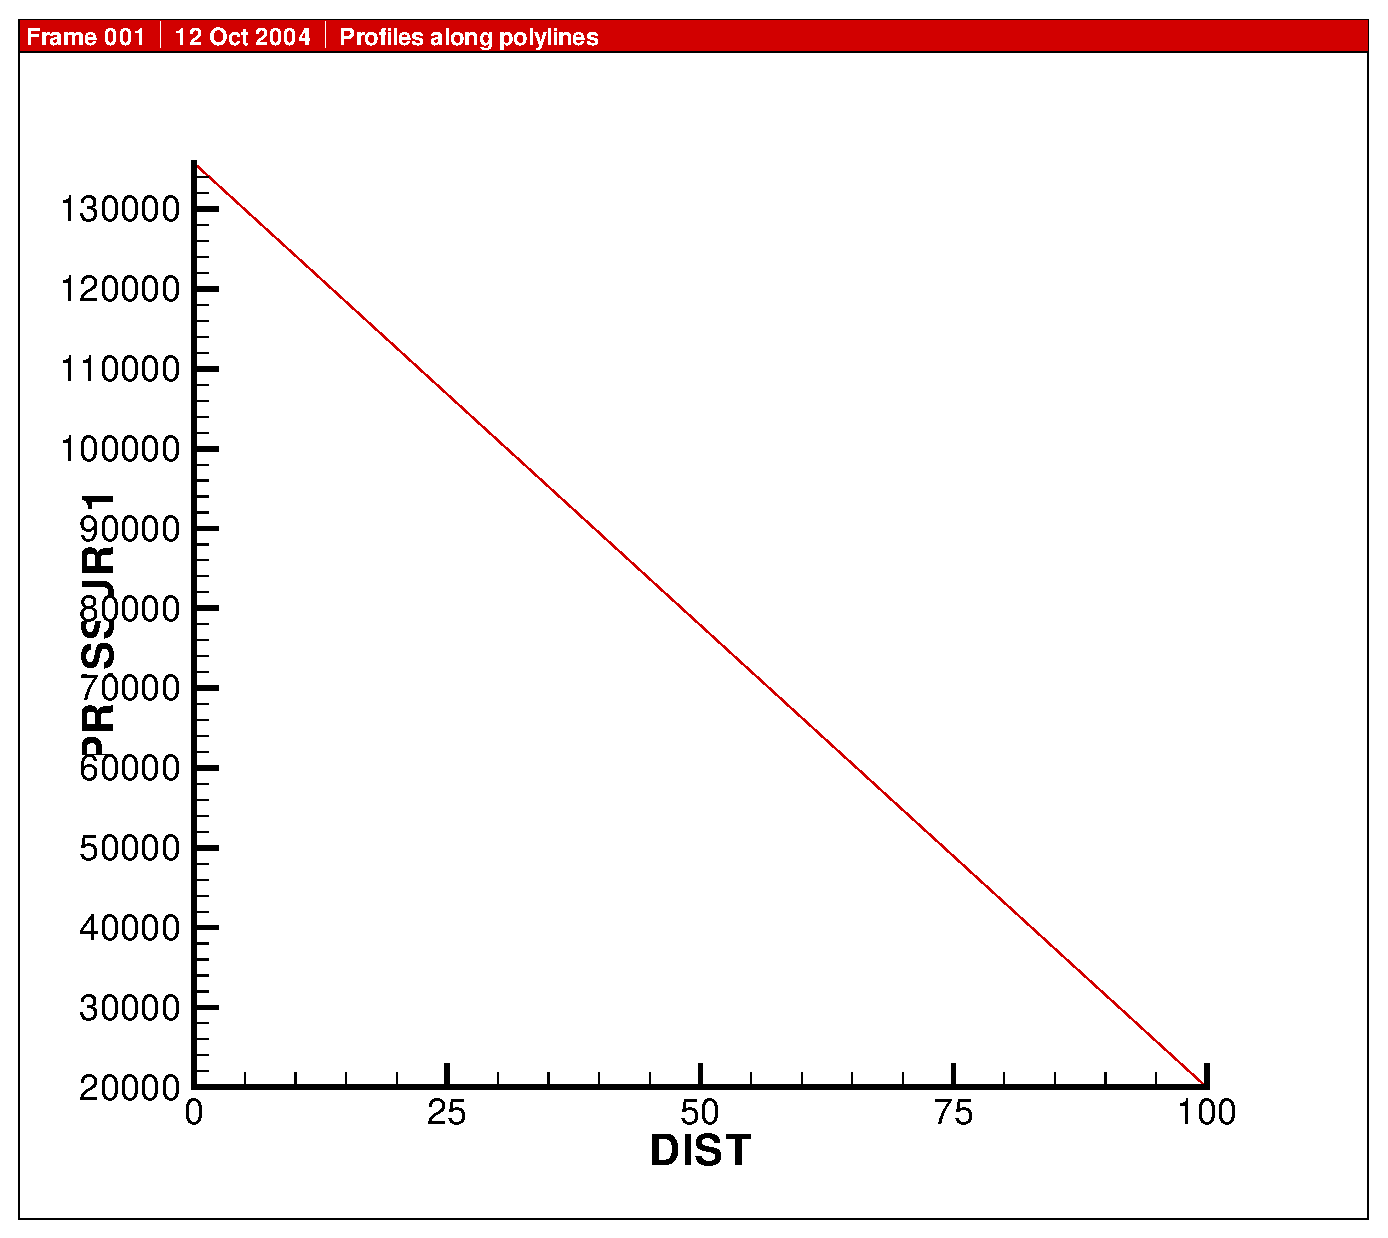
\includegraphics[width=7cm]{figures/h_line.eps}\\
  %\caption{}\label{}
\end{figure}

\begin{figure}[htb!]
  % Requires \usepackage{graphicx}
  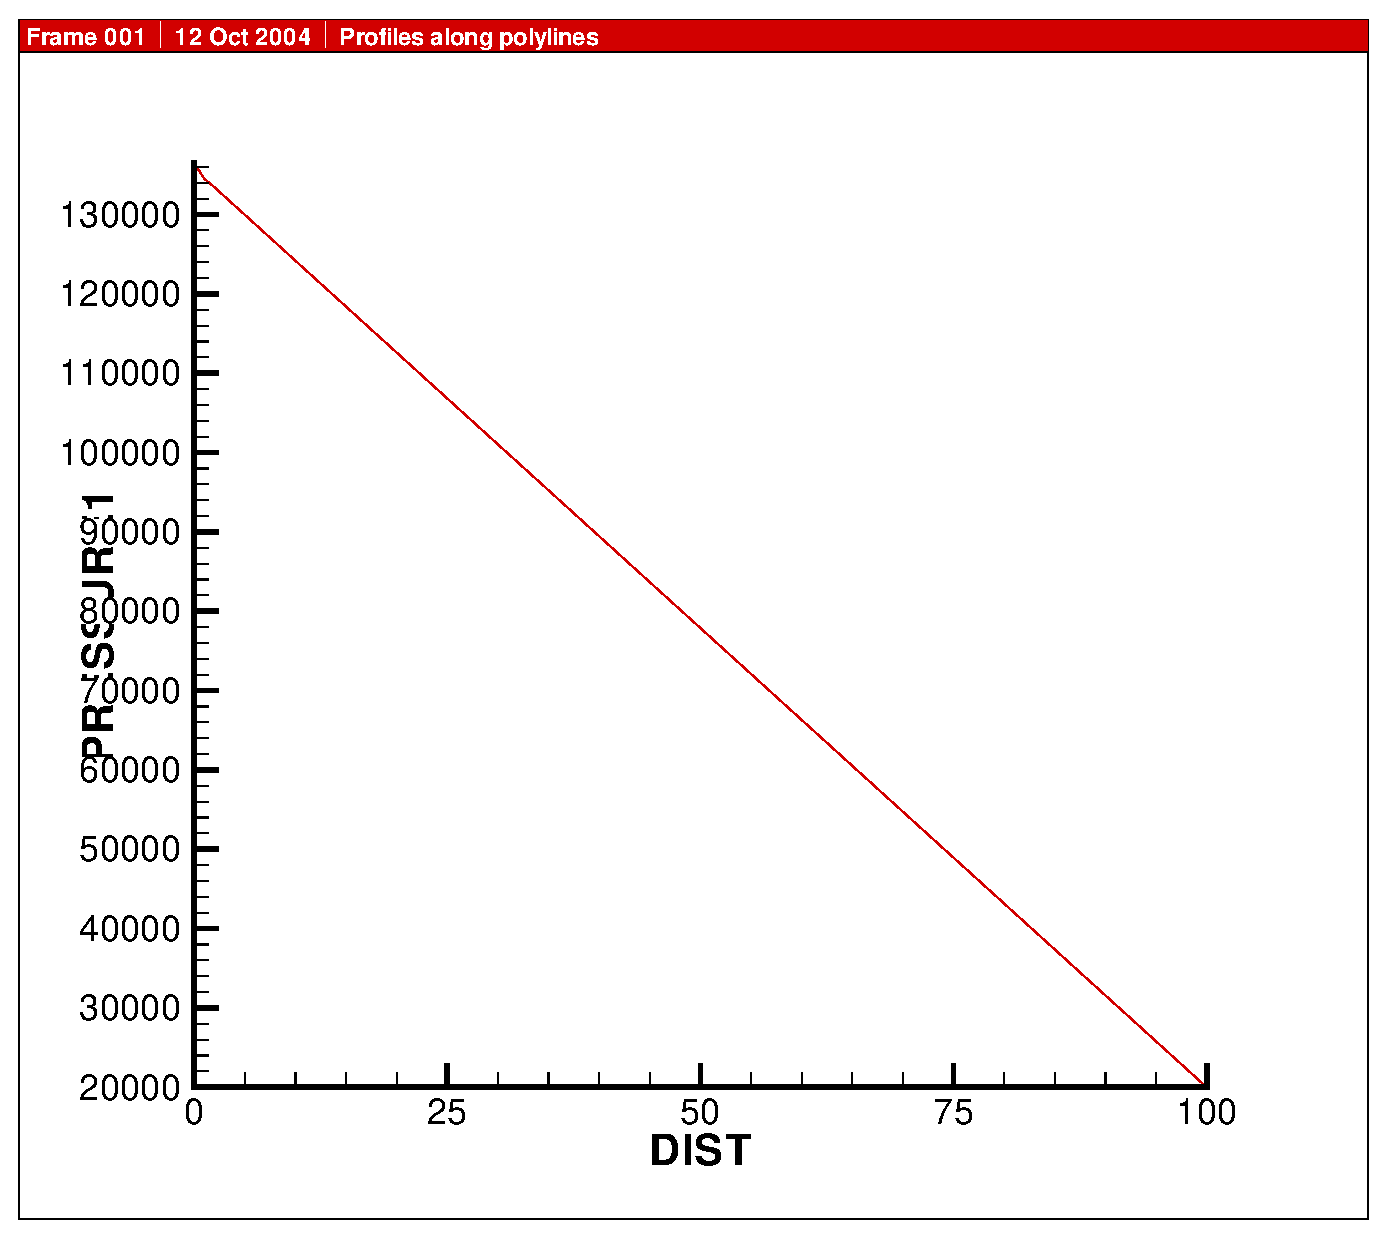
\includegraphics[width=7cm]{figures/h_quad.eps}\\
  %\caption{}\label{}
\end{figure}

\begin{figure}[htb!]
  % Requires \usepackage{graphicx}
  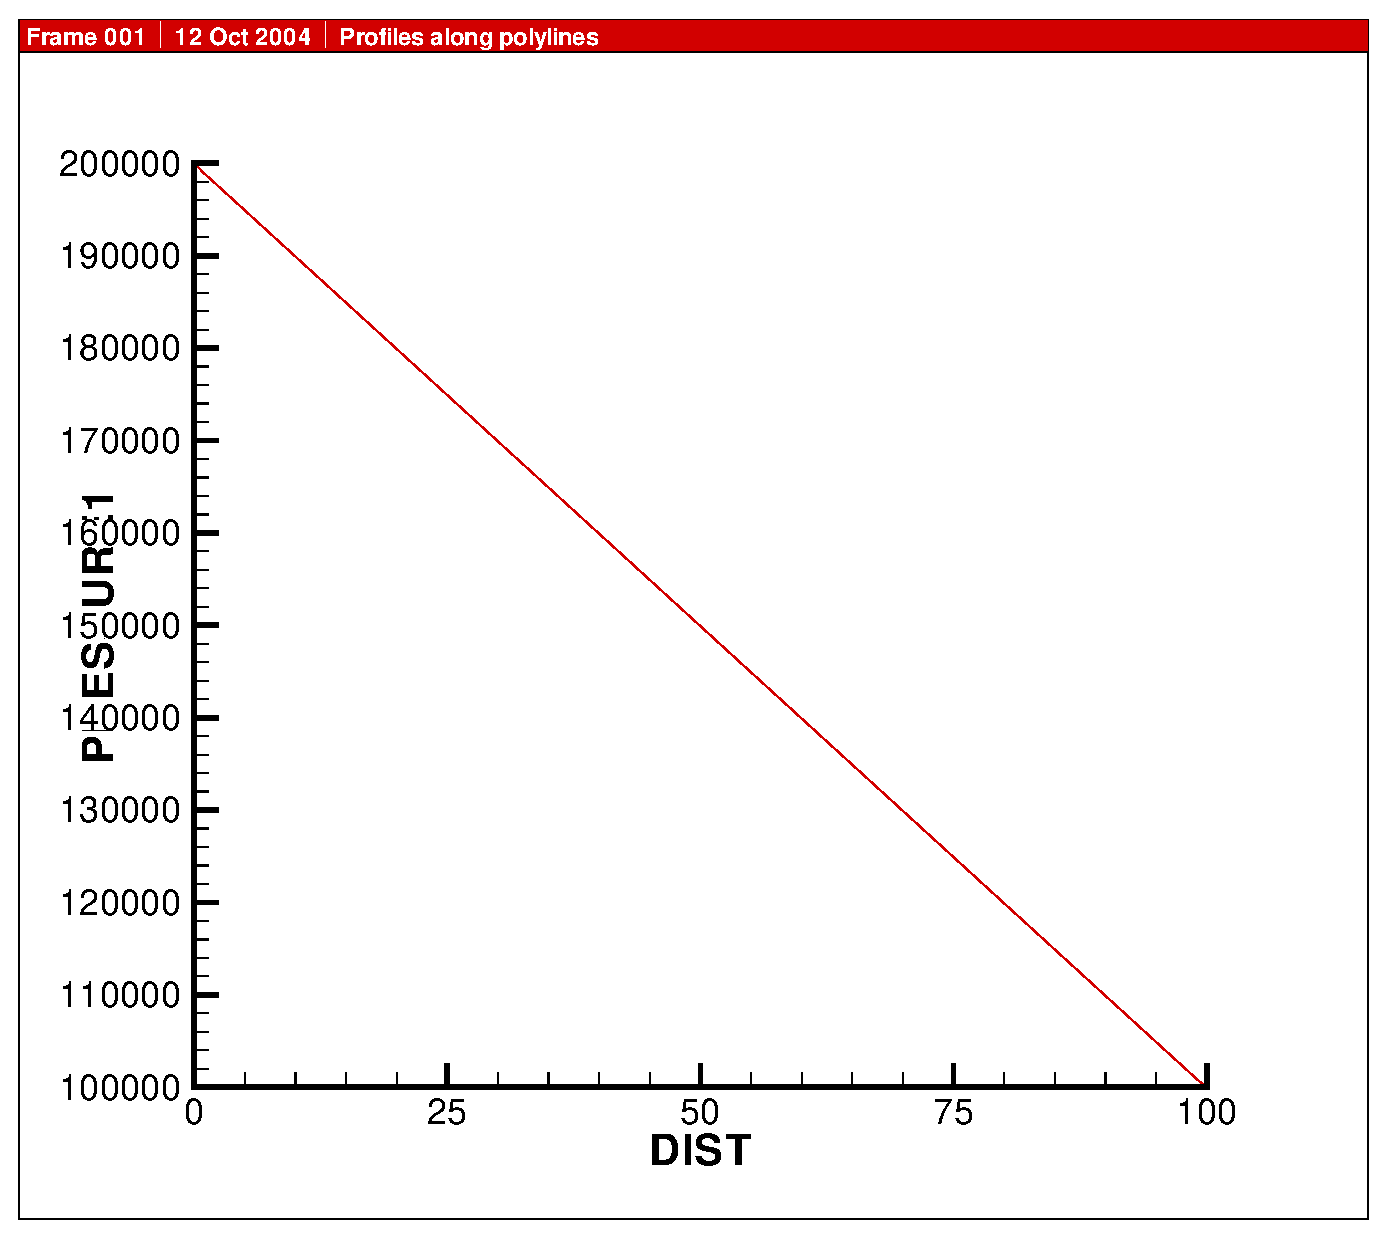
\includegraphics[width=7cm]{figures/h_hex.eps}\\
  %\caption{}\label{}
\end{figure}

\begin{figure}[htb!]
  % Requires \usepackage{graphicx}
  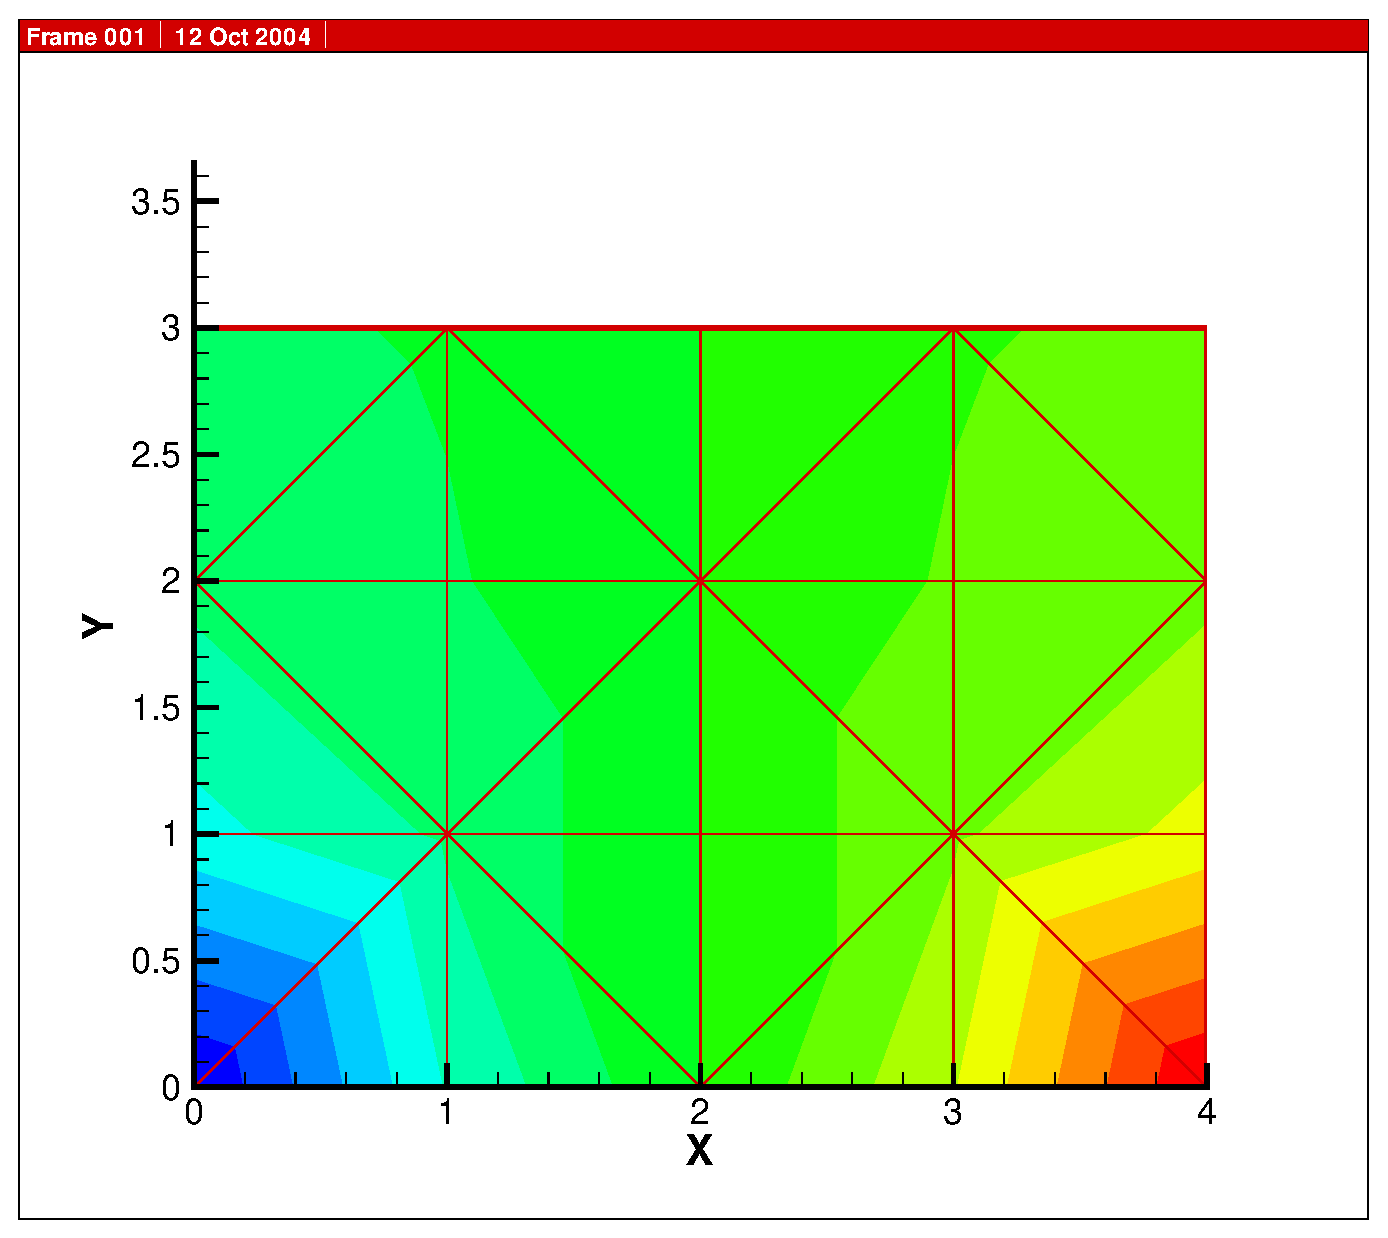
\includegraphics[width=7cm]{figures/h_tri.eps}\\
  %\caption{}\label{}
\end{figure}

\begin{figure}[htb!]
  % Requires \usepackage{graphicx}
  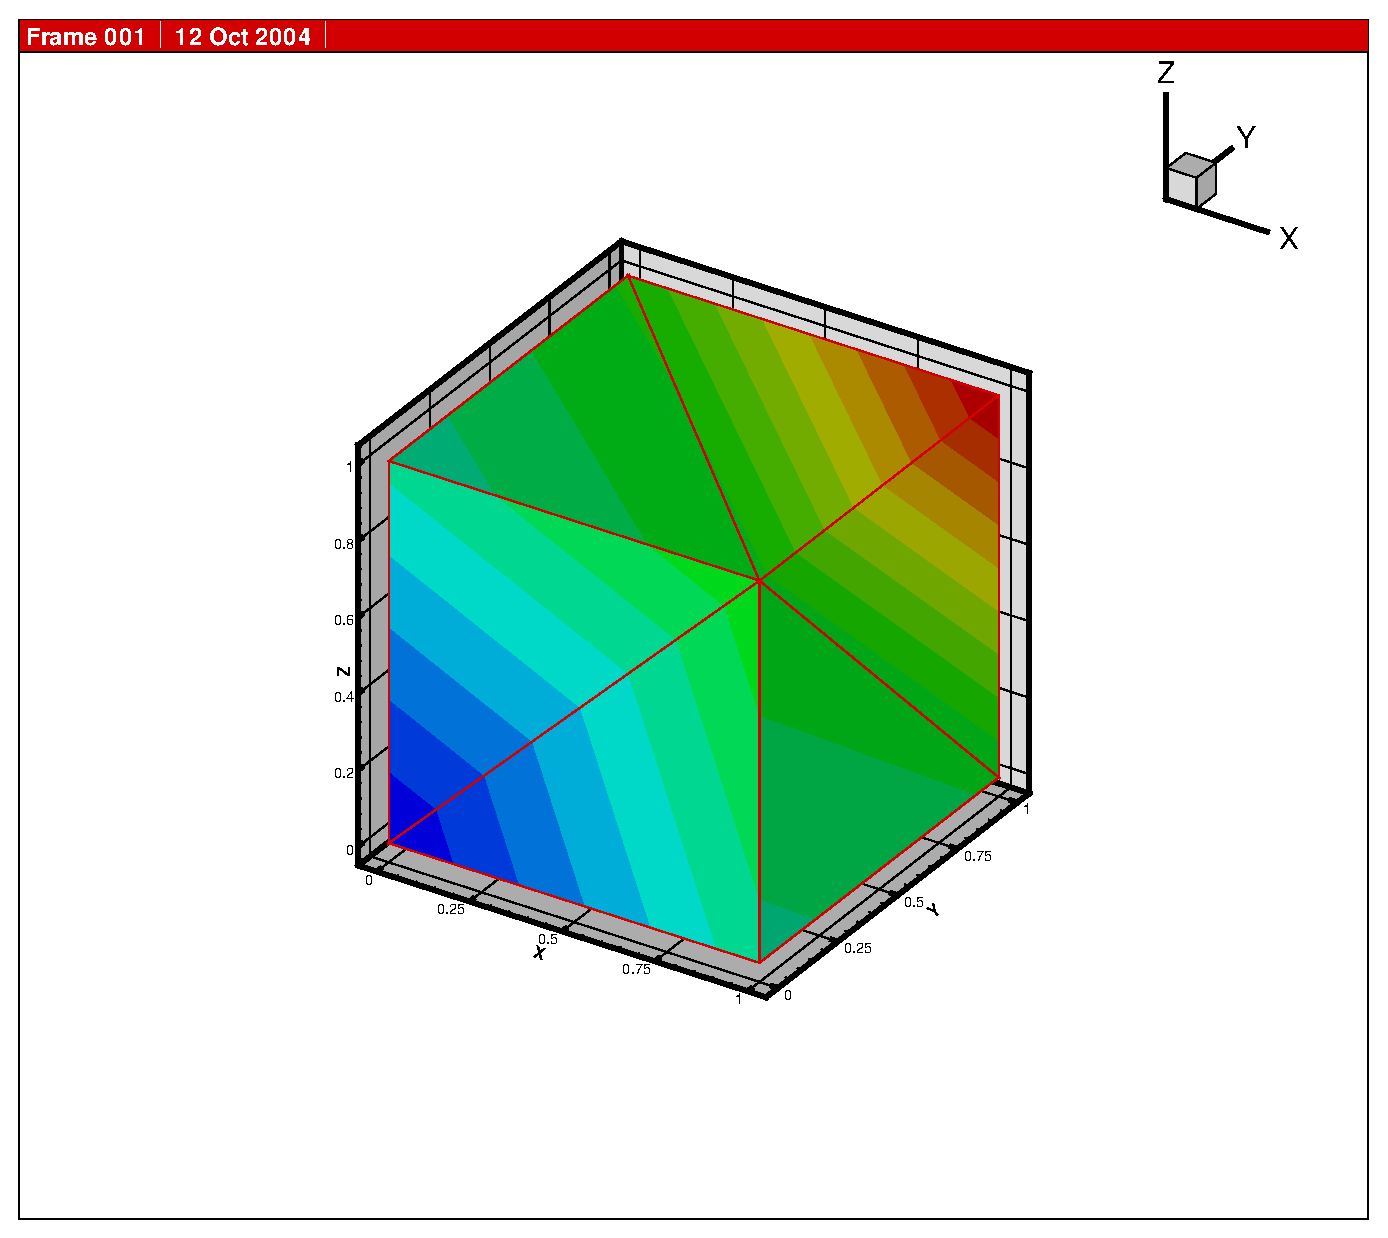
\includegraphics[width=7cm]{figures/h_tet1.eps}\\
  %\caption{}\label{}
\end{figure}

\begin{figure}[htb!]
  % Requires \usepackage{graphicx}
  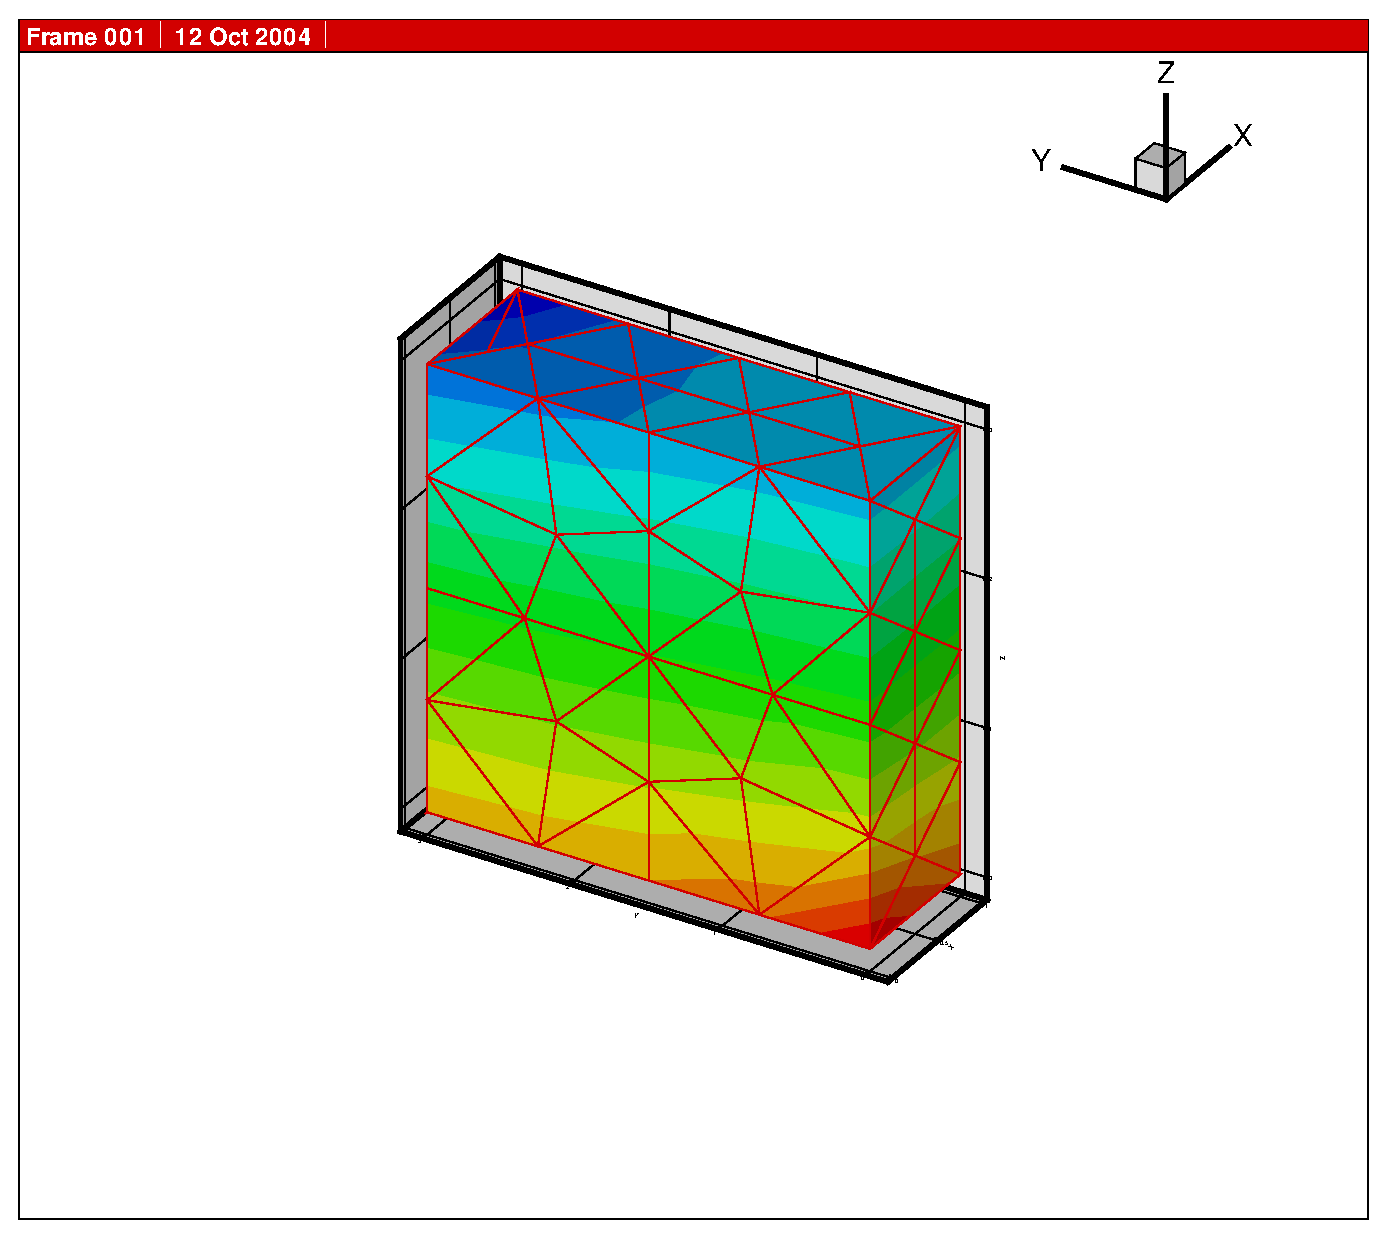
\includegraphics[width=7cm]{figures/h_tet2.eps}\\
  %\caption{}\label{}
\end{figure}

\begin{figure}[htb!]
  % Requires \usepackage{graphicx}
  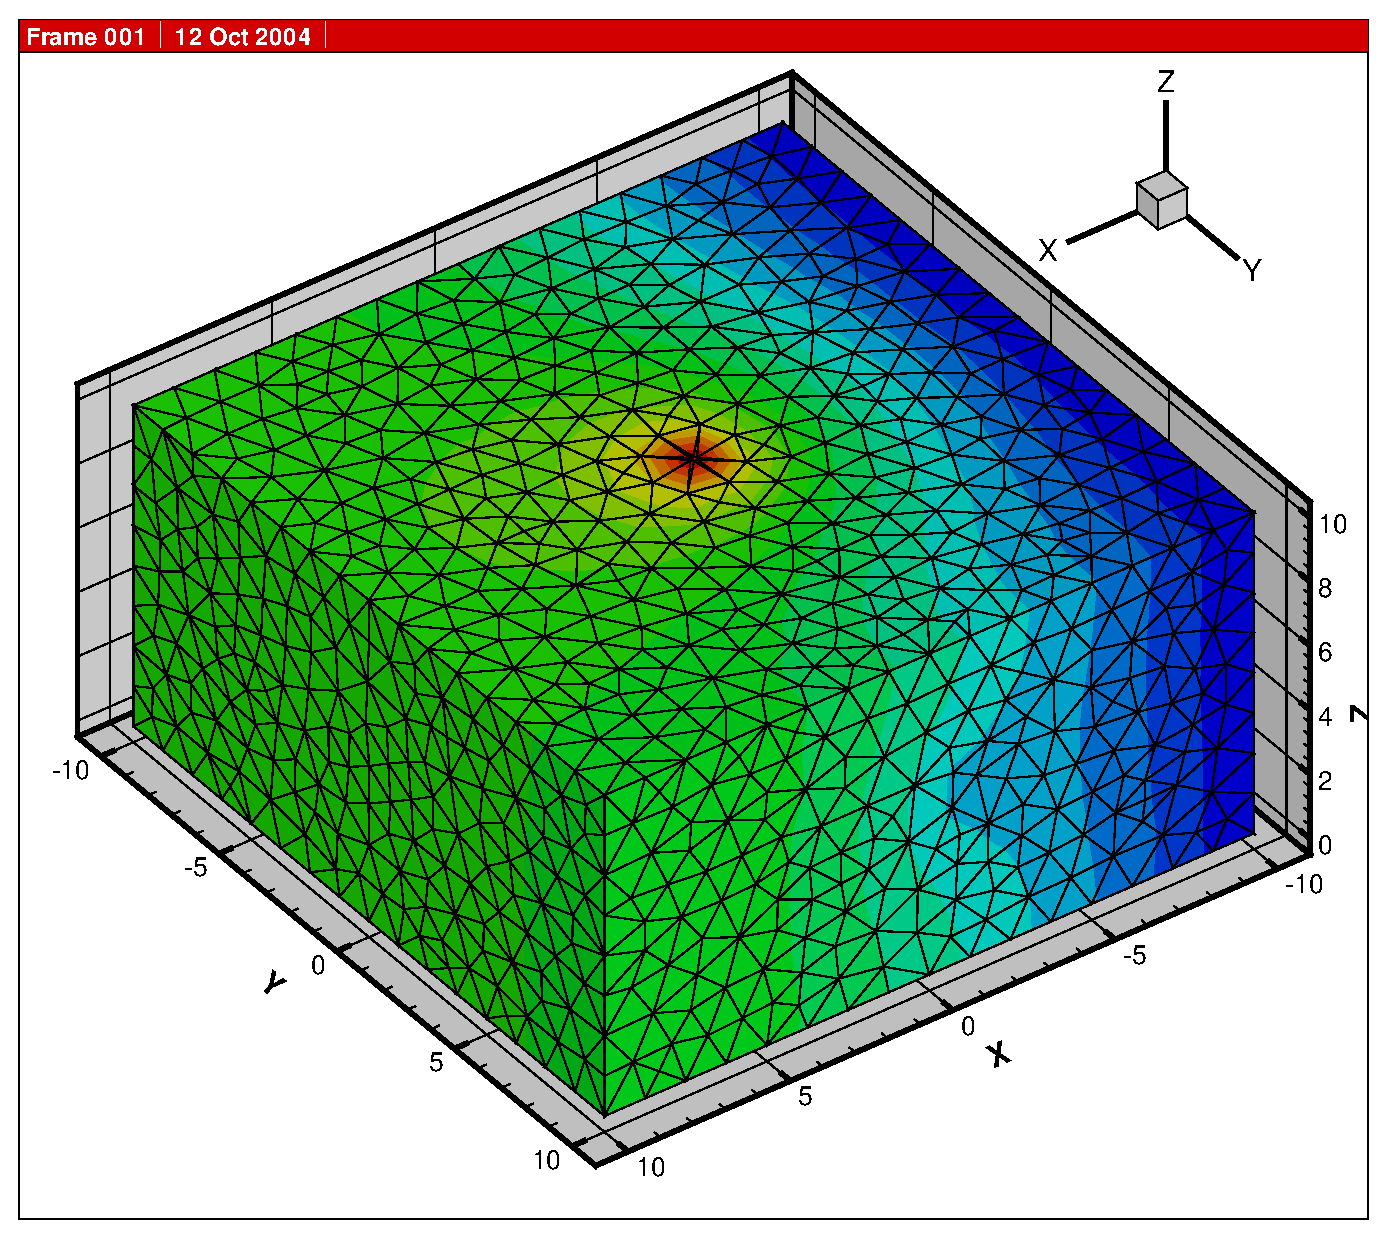
\includegraphics[width=7cm]{figures/h_tet3.eps}\\
  %\caption{}\label{}
\end{figure}

\newpage $ $ \newpage
\subsection{Unconfined Groundwater Flow}

\begin{figure}[htb!]
  % Requires \usepackage{graphicx}
  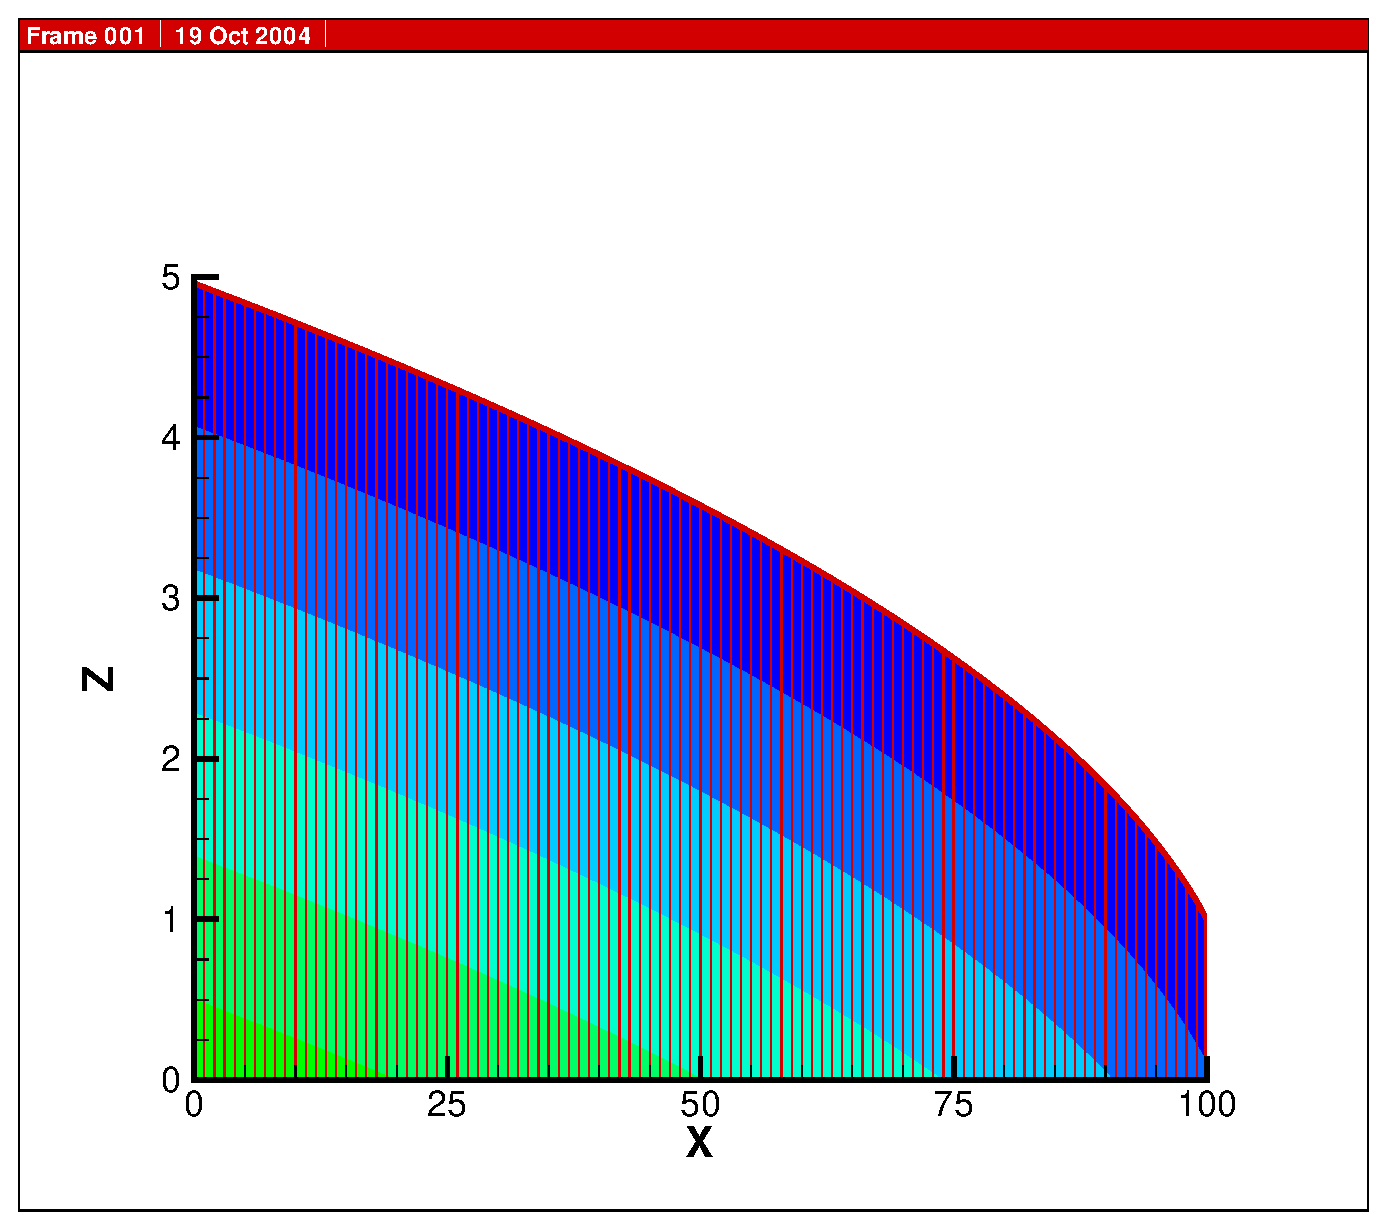
\includegraphics[width=7cm]{figures/h_uc_quad.eps}\\
  %\caption{}\label{}
\end{figure}

\begin{figure}[htb!]
  % Requires \usepackage{graphicx}
  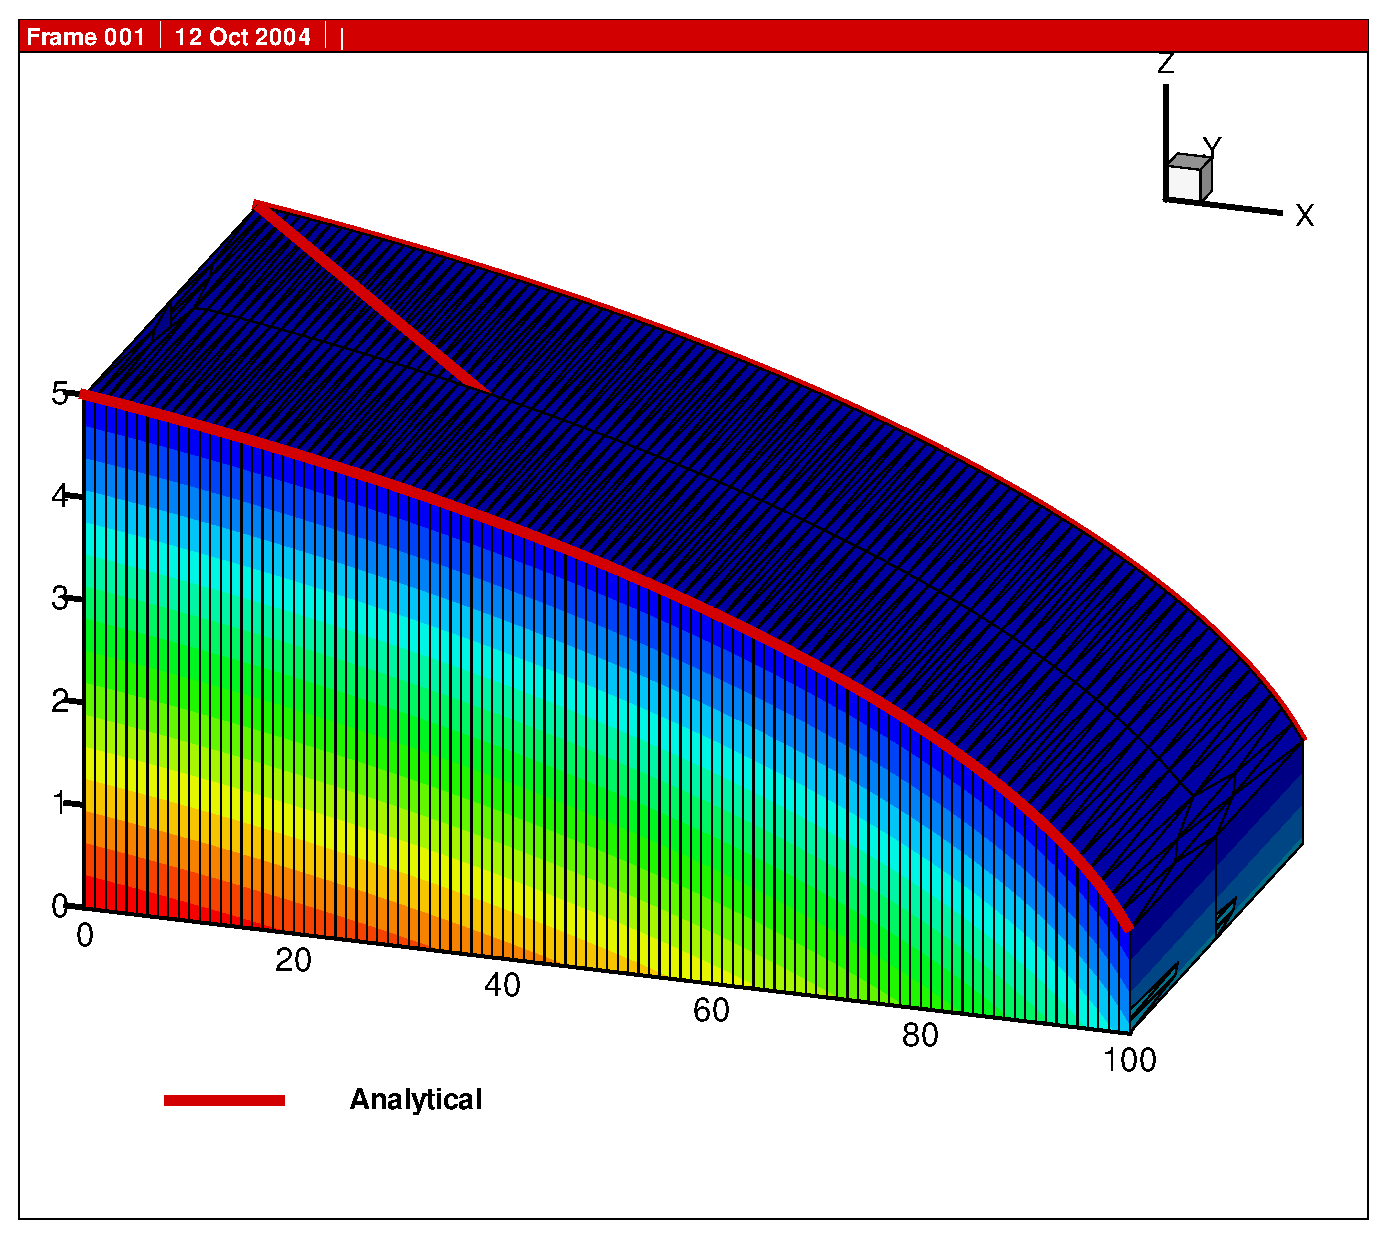
\includegraphics[width=7cm]{figures/h_uc_pris.eps}\\
  %\caption{}\label{}
\end{figure}

\newpage
\subsection{Gas Flow}

\begin{figure}[htb!]
  % Requires \usepackage{graphicx}
  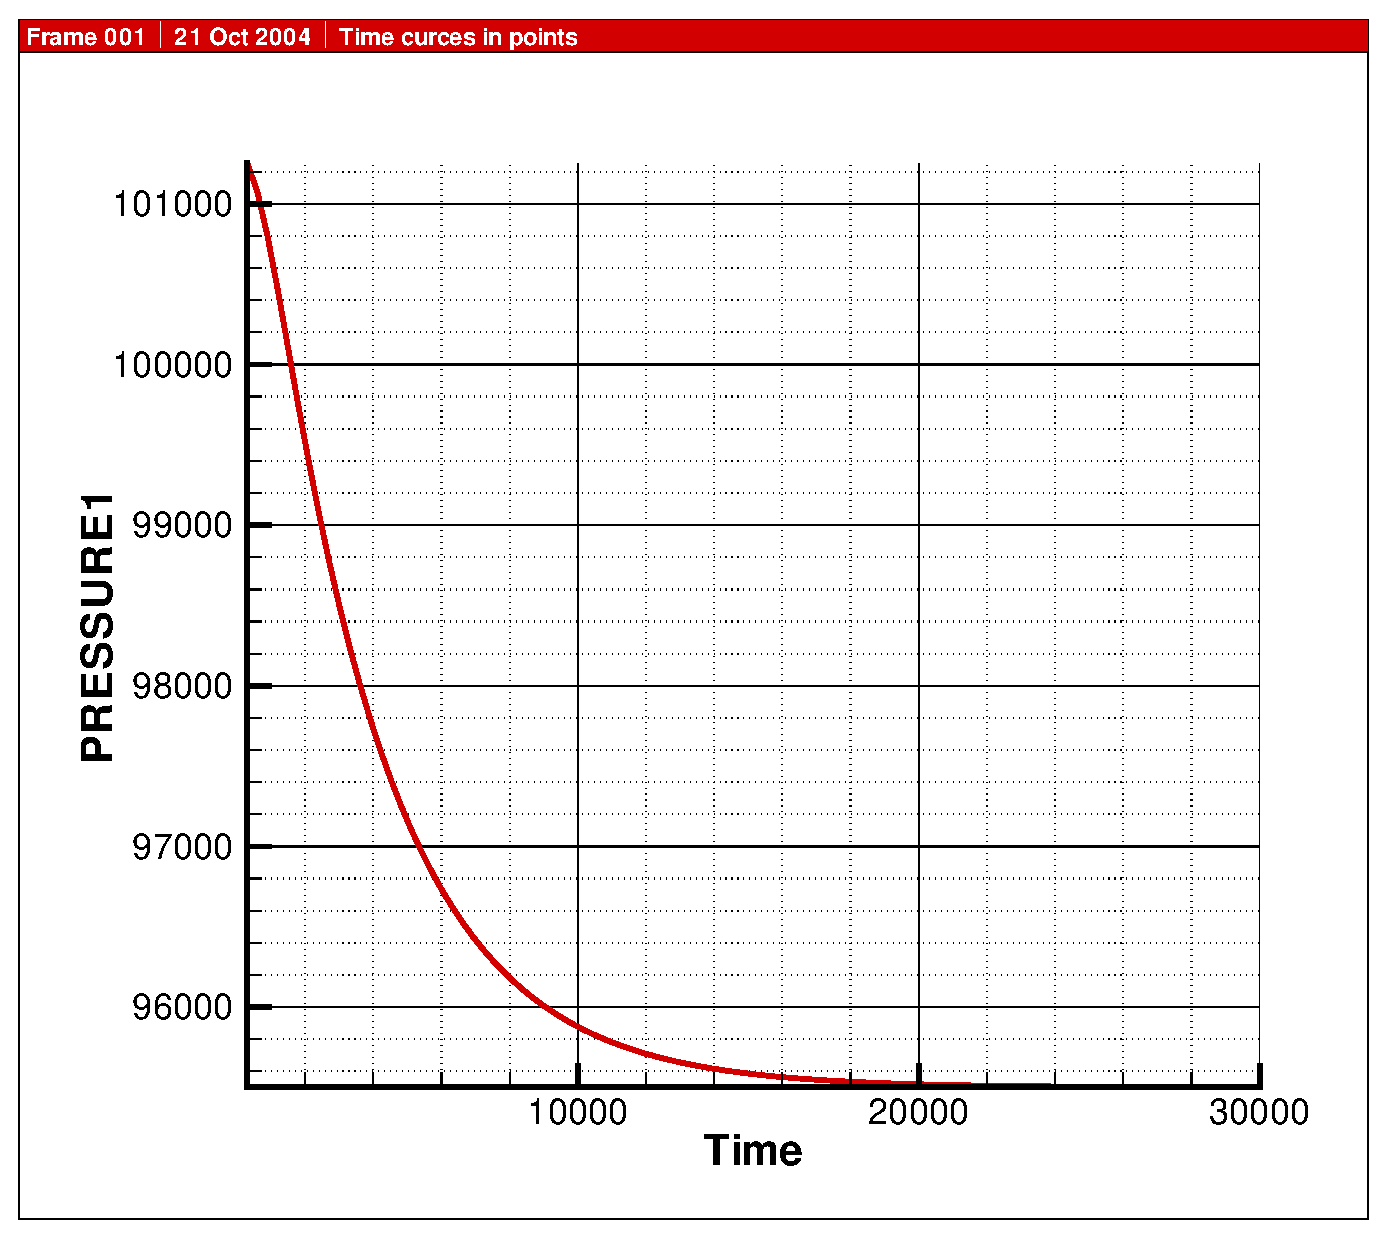
\includegraphics[width=7cm]{figures/h_gas_line.eps}\\
  %\caption{}\label{}
\end{figure}

\begin{figure}[htb!]
  % Requires \usepackage{graphicx}
  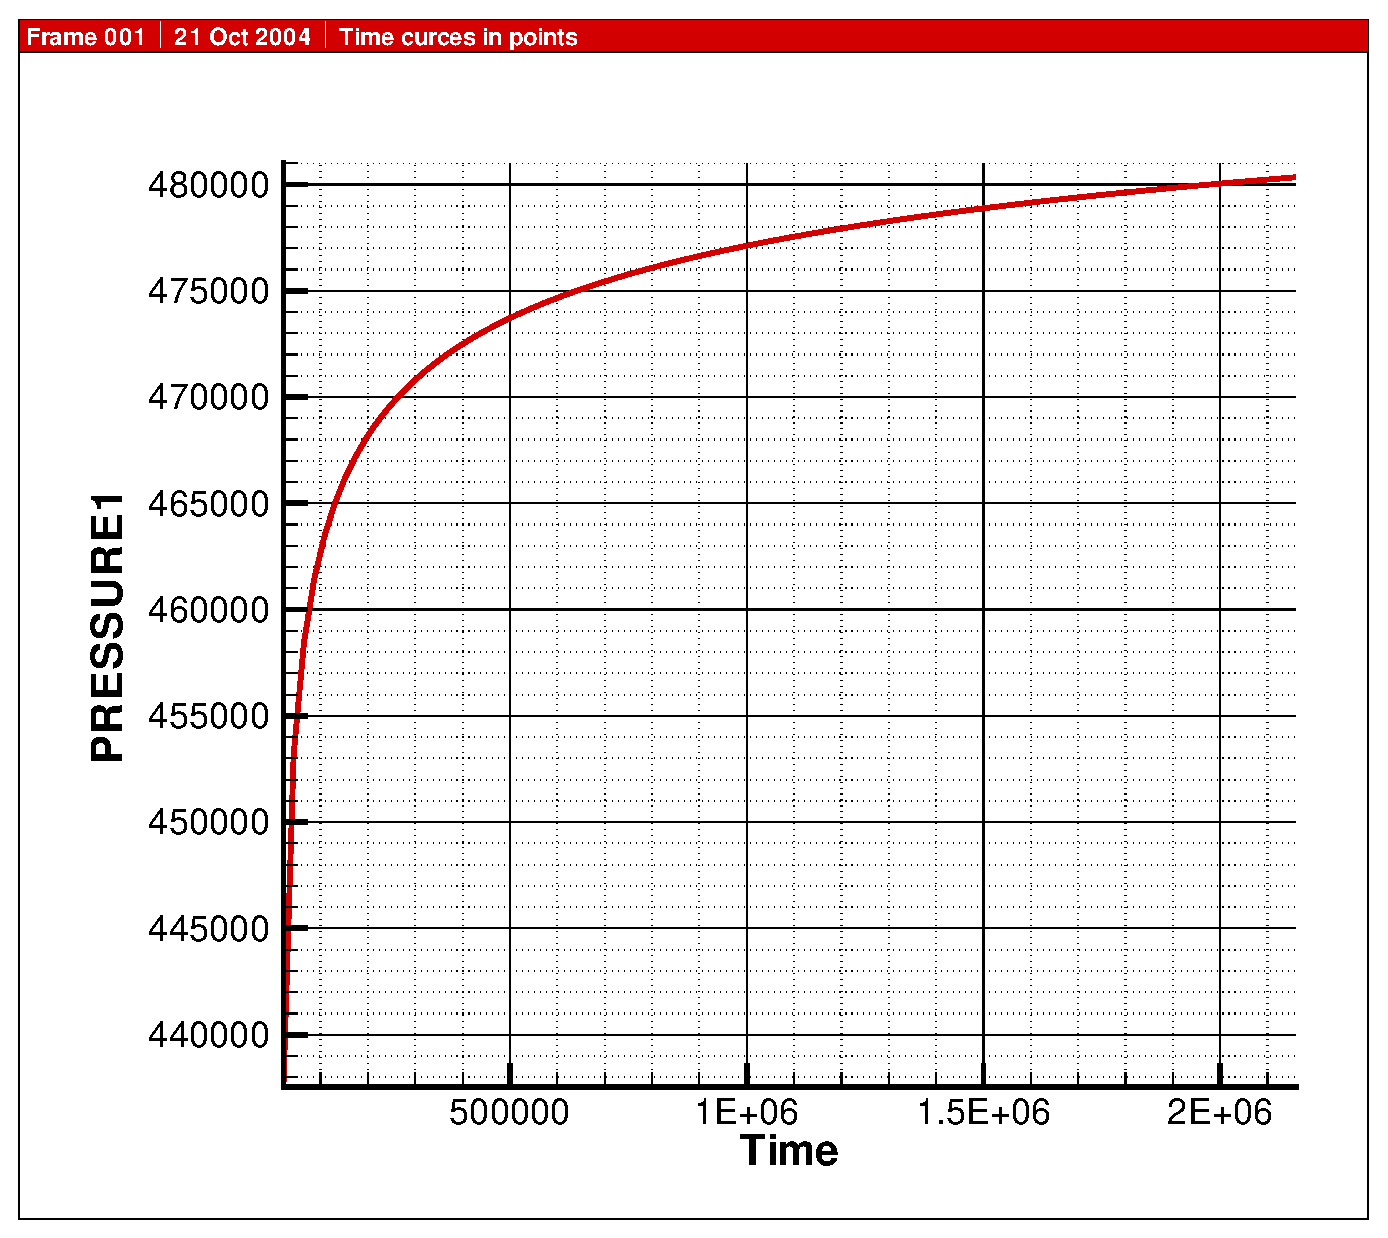
\includegraphics[width=7cm]{figures/h_gas_quad.eps}\\
  %\caption{}\label{}
\end{figure}

\newpage
\subsection{Two-Phase Flow}

\begin{figure}[htb!]
  % Requires \usepackage{graphicx}
  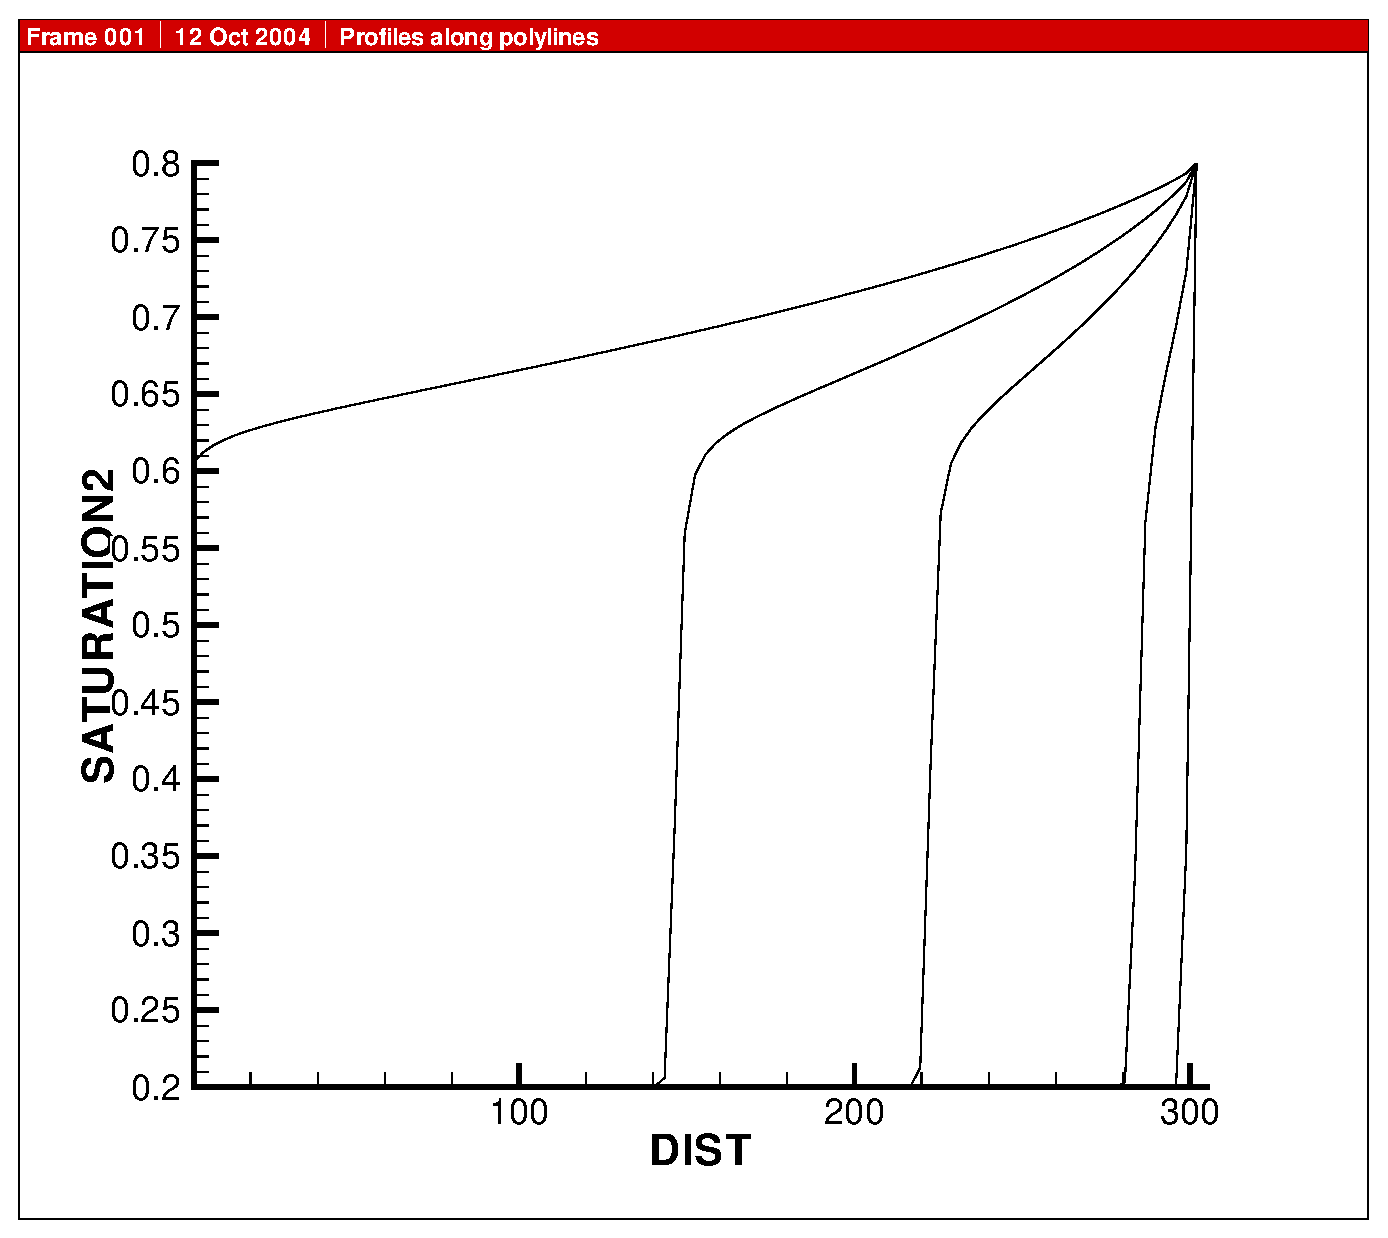
\includegraphics[width=7cm]{figures/h2_line.eps}\\
  %\caption{}\label{}
\end{figure}

\newpage
\subsection{Heat Transport}

\begin{figure}[htb!]
  % Requires \usepackage{graphicx}
  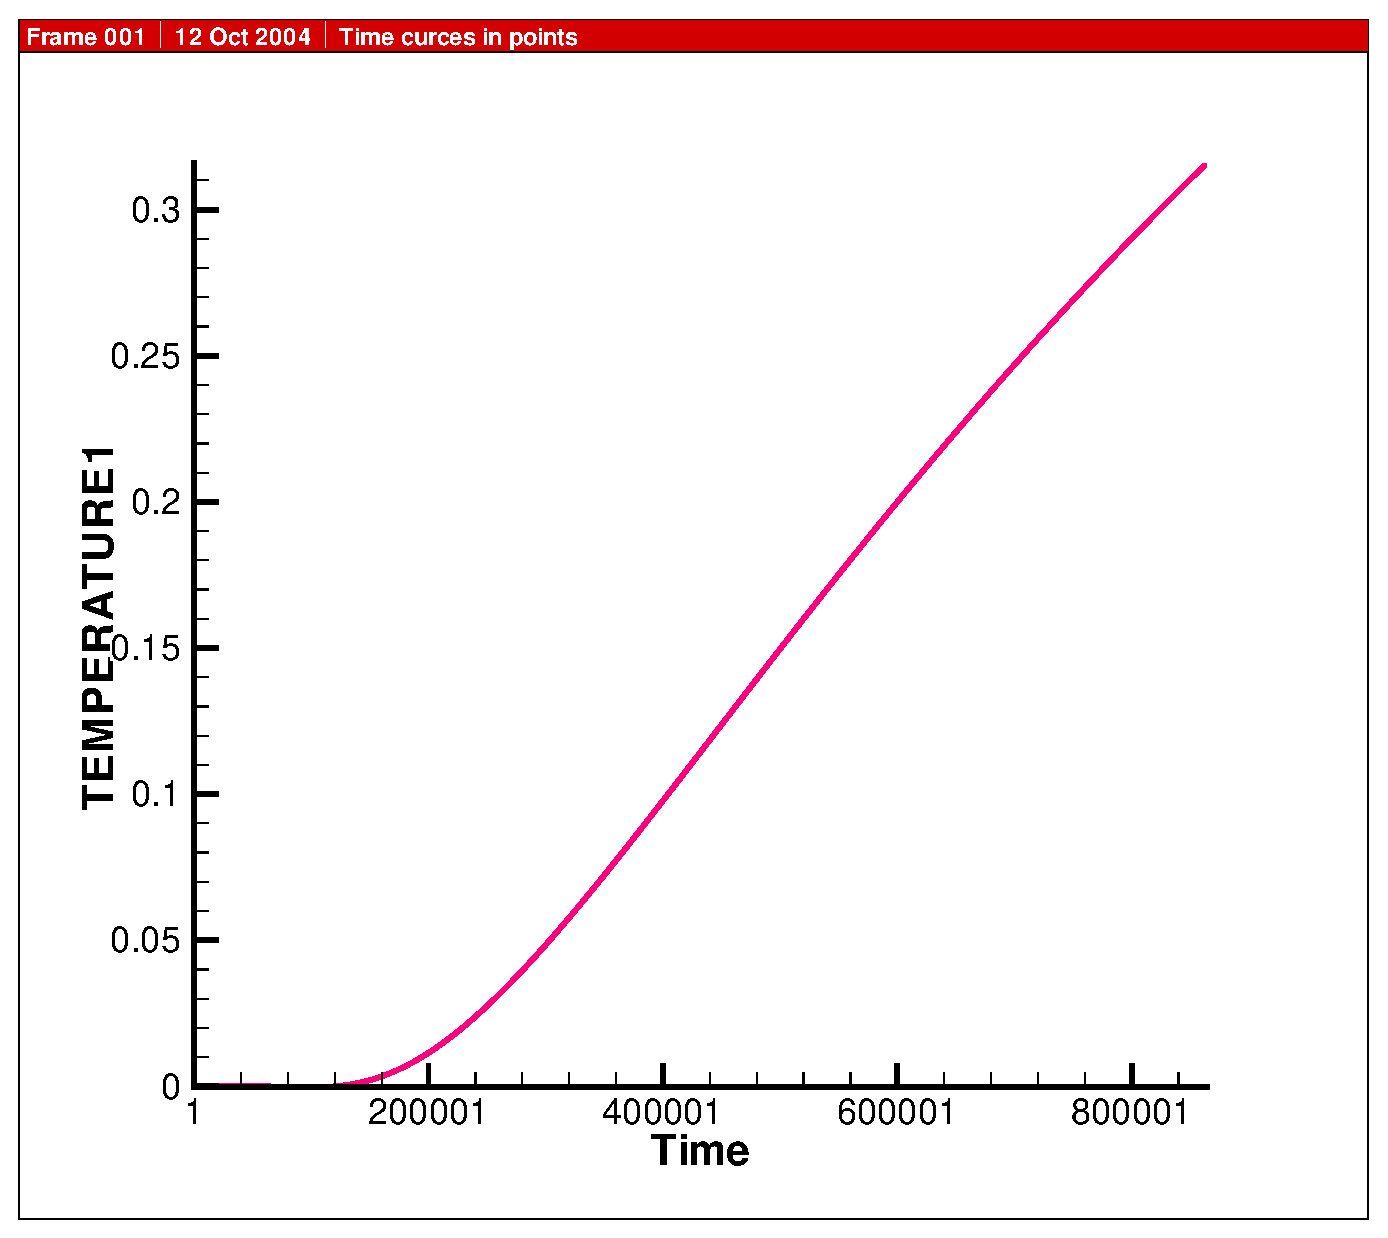
\includegraphics[width=7cm]{figures/ht_line.eps}\\
  %\caption{}\label{}
\end{figure}

\begin{figure}[htb!]
  % Requires \usepackage{graphicx}
  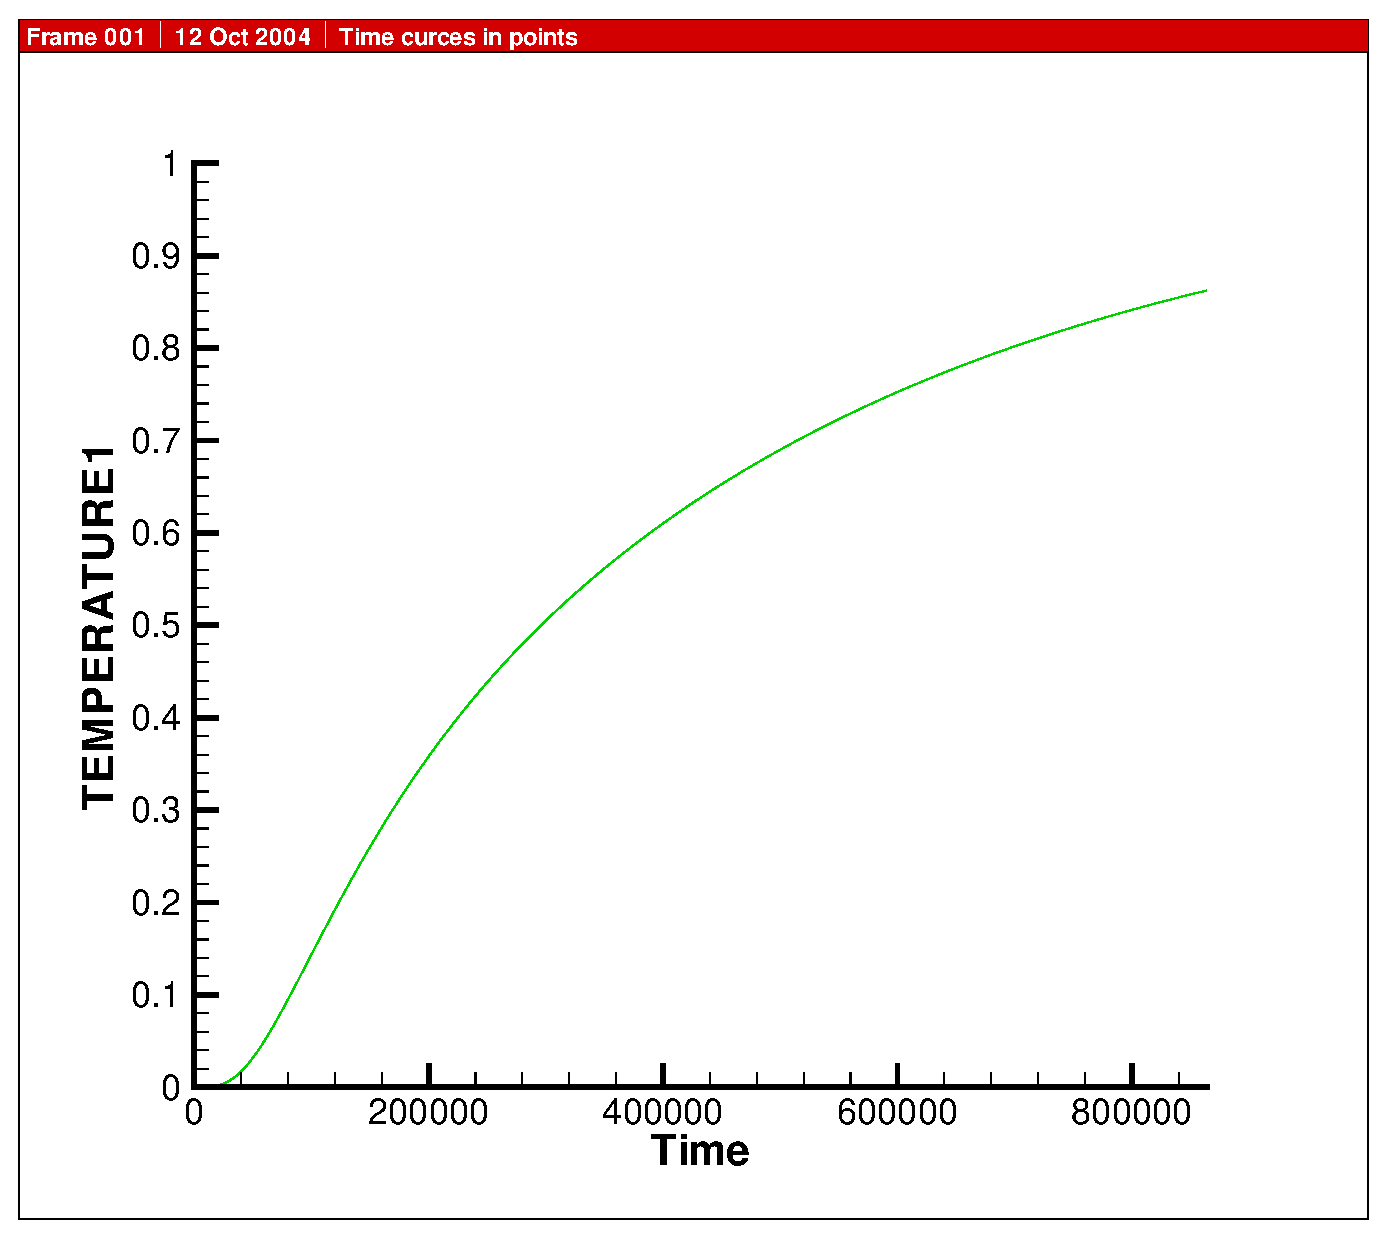
\includegraphics[width=7cm]{figures/ht_tri.eps}\\
  %\caption{}\label{}
\end{figure}

\begin{figure}[htb!]
  % Requires \usepackage{graphicx}
  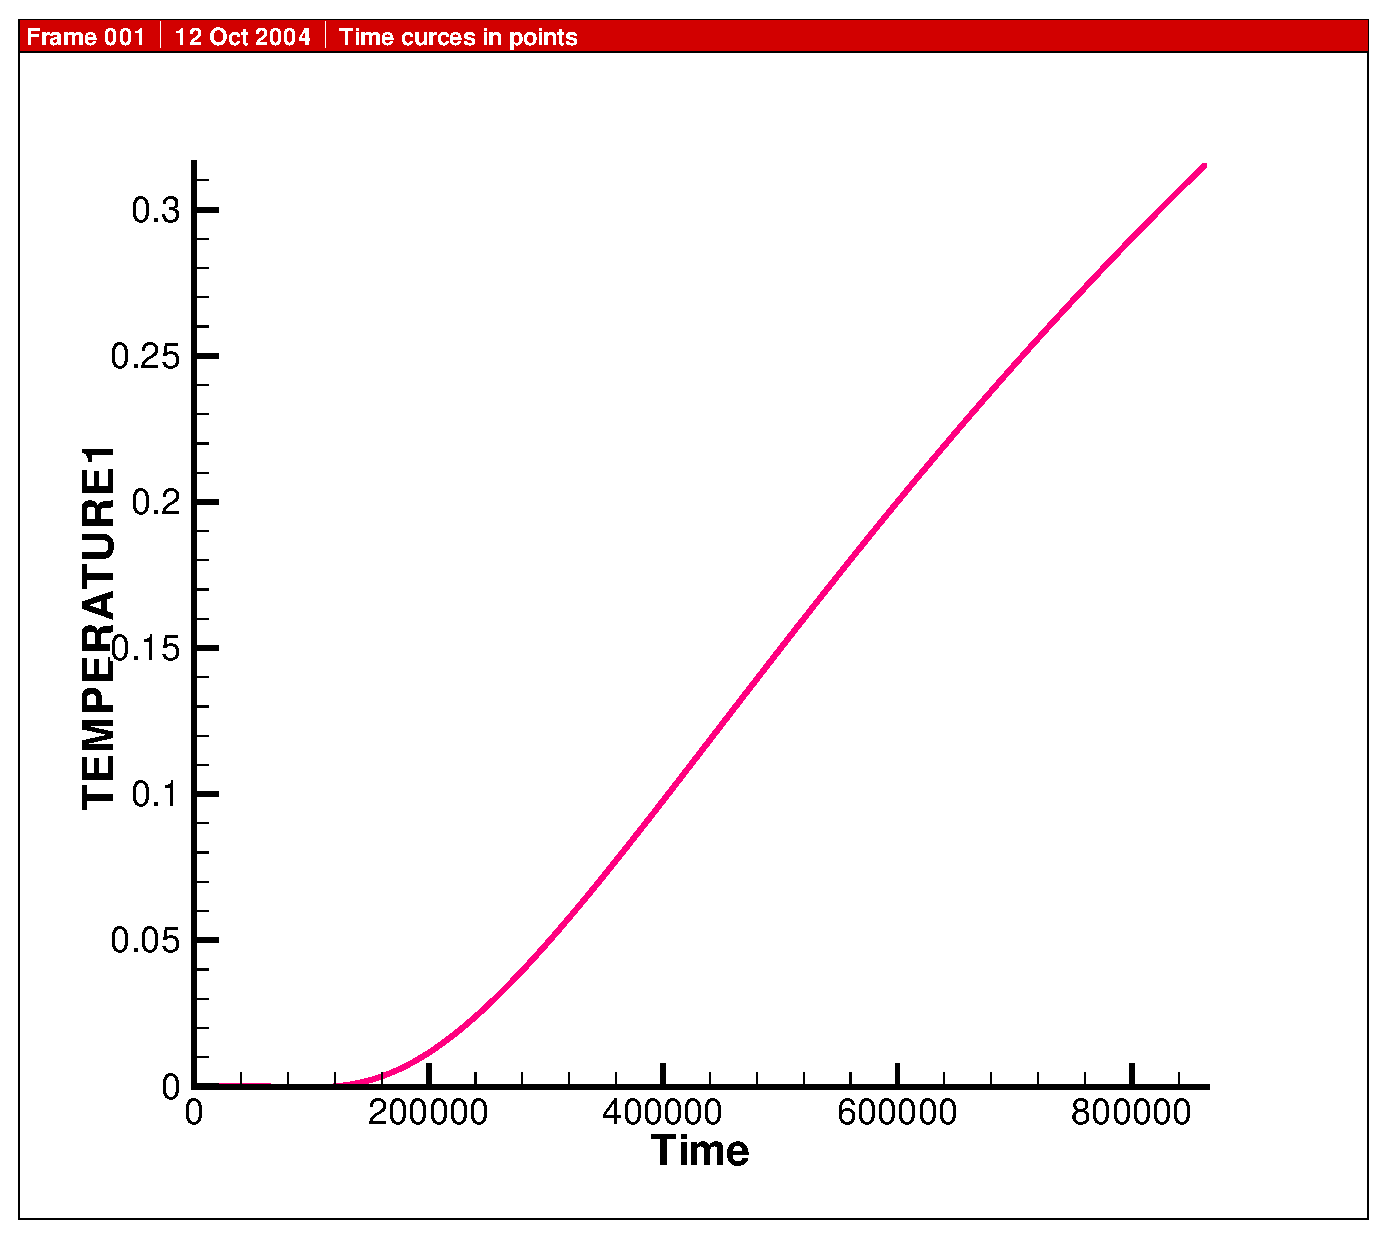
\includegraphics[width=7cm]{figures/ht_quad.eps}\\
  %\caption{}\label{}
\end{figure}

\begin{figure}[htb!]
  % Requires \usepackage{graphicx}
  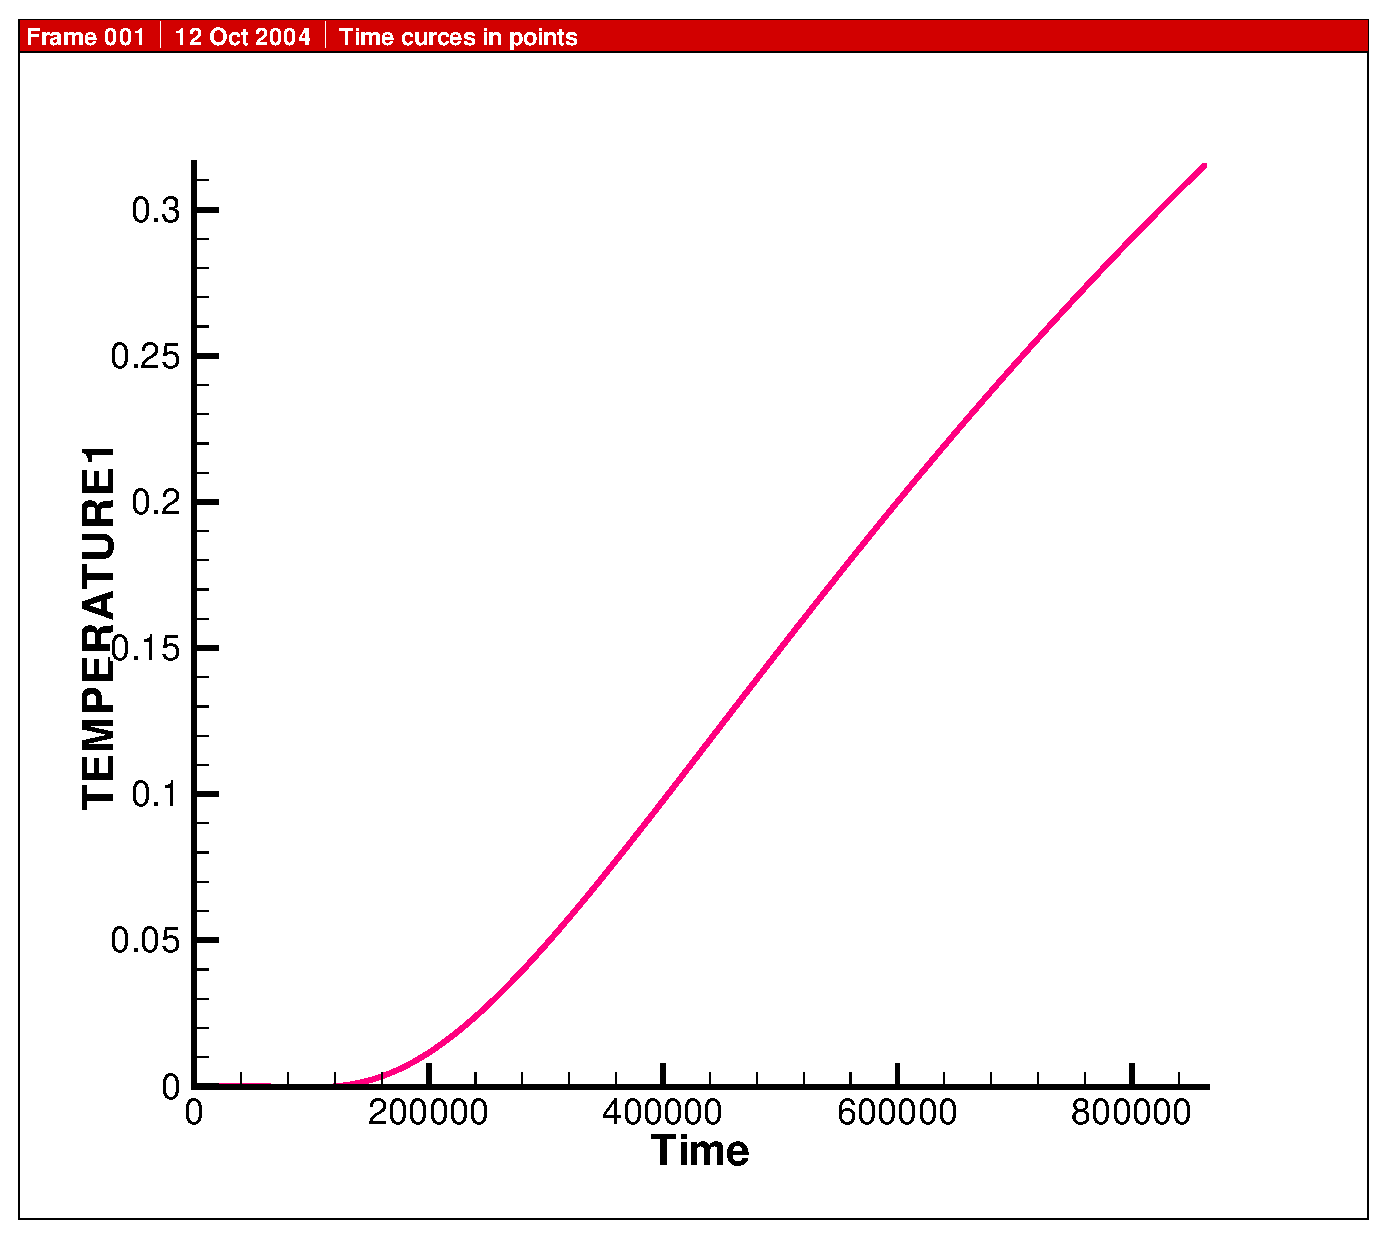
\includegraphics[width=7cm]{figures/ht_hex.eps}\\
  %\caption{}\label{}
\end{figure}

\begin{figure}[htb!]
  % Requires \usepackage{graphicx}
  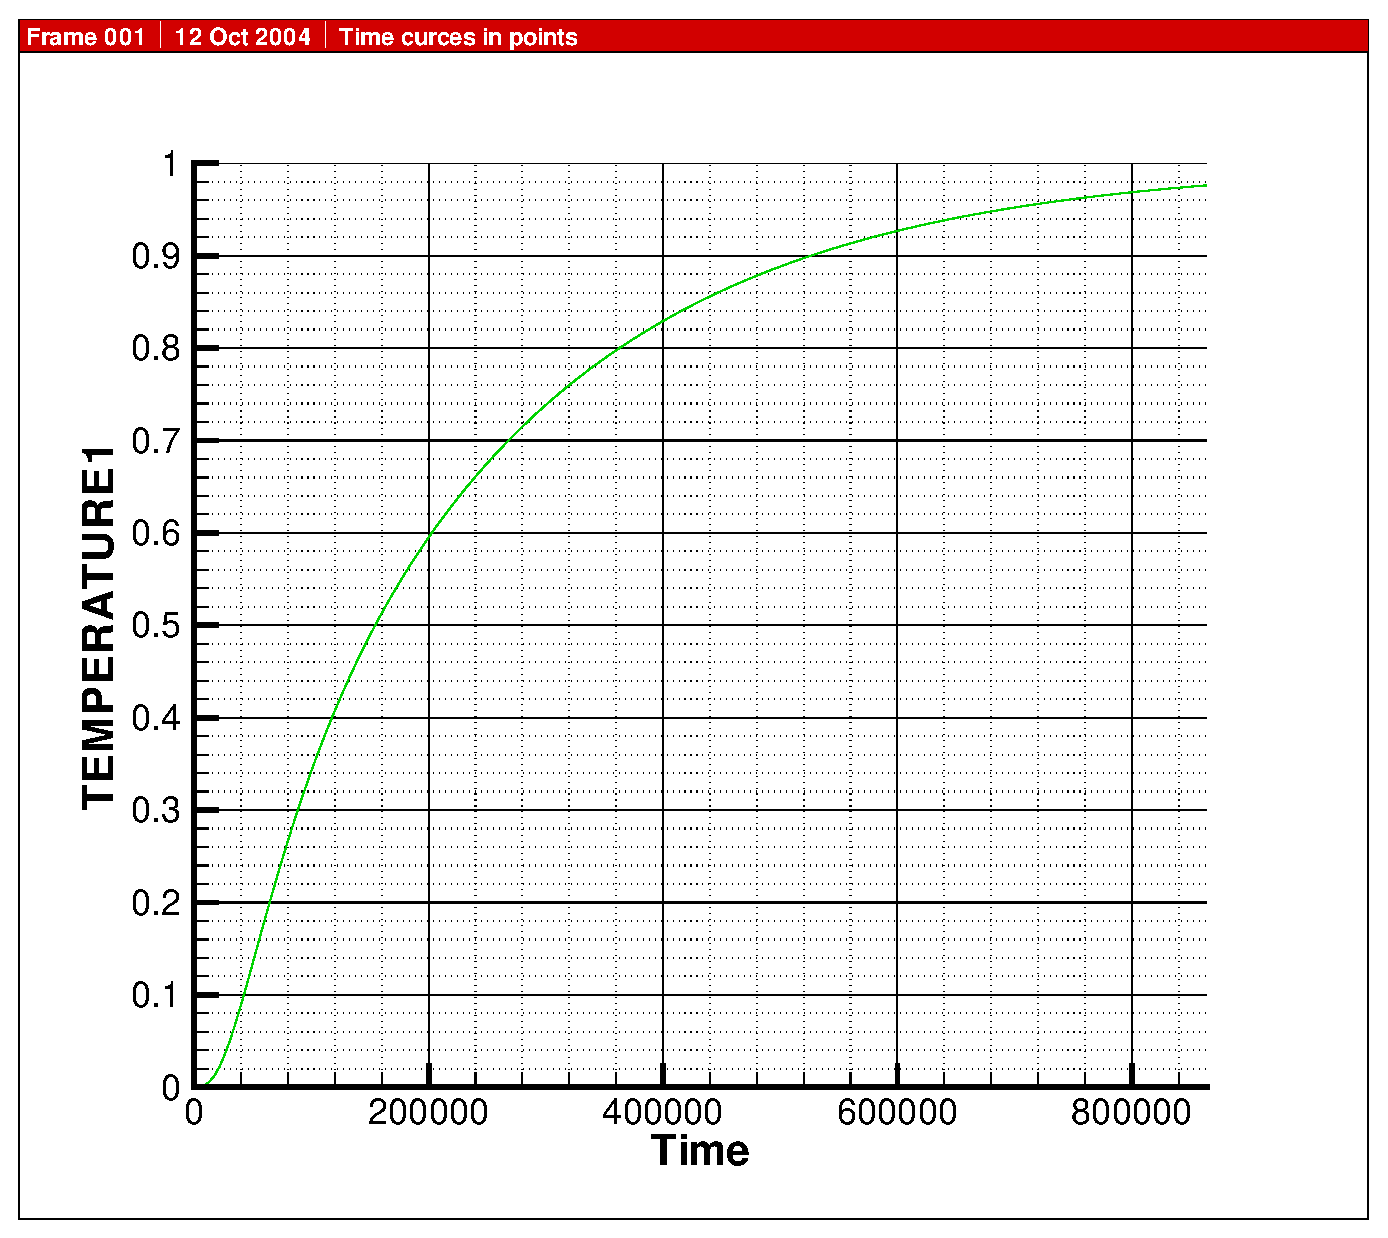
\includegraphics[width=7cm]{figures/ht_pris.eps}\\
  %\caption{}\label{}
\end{figure}

\newpage $ $ \newpage
\subsection{Deformation}

\begin{figure}[htb!]
  % Requires \usepackage{graphicx}
  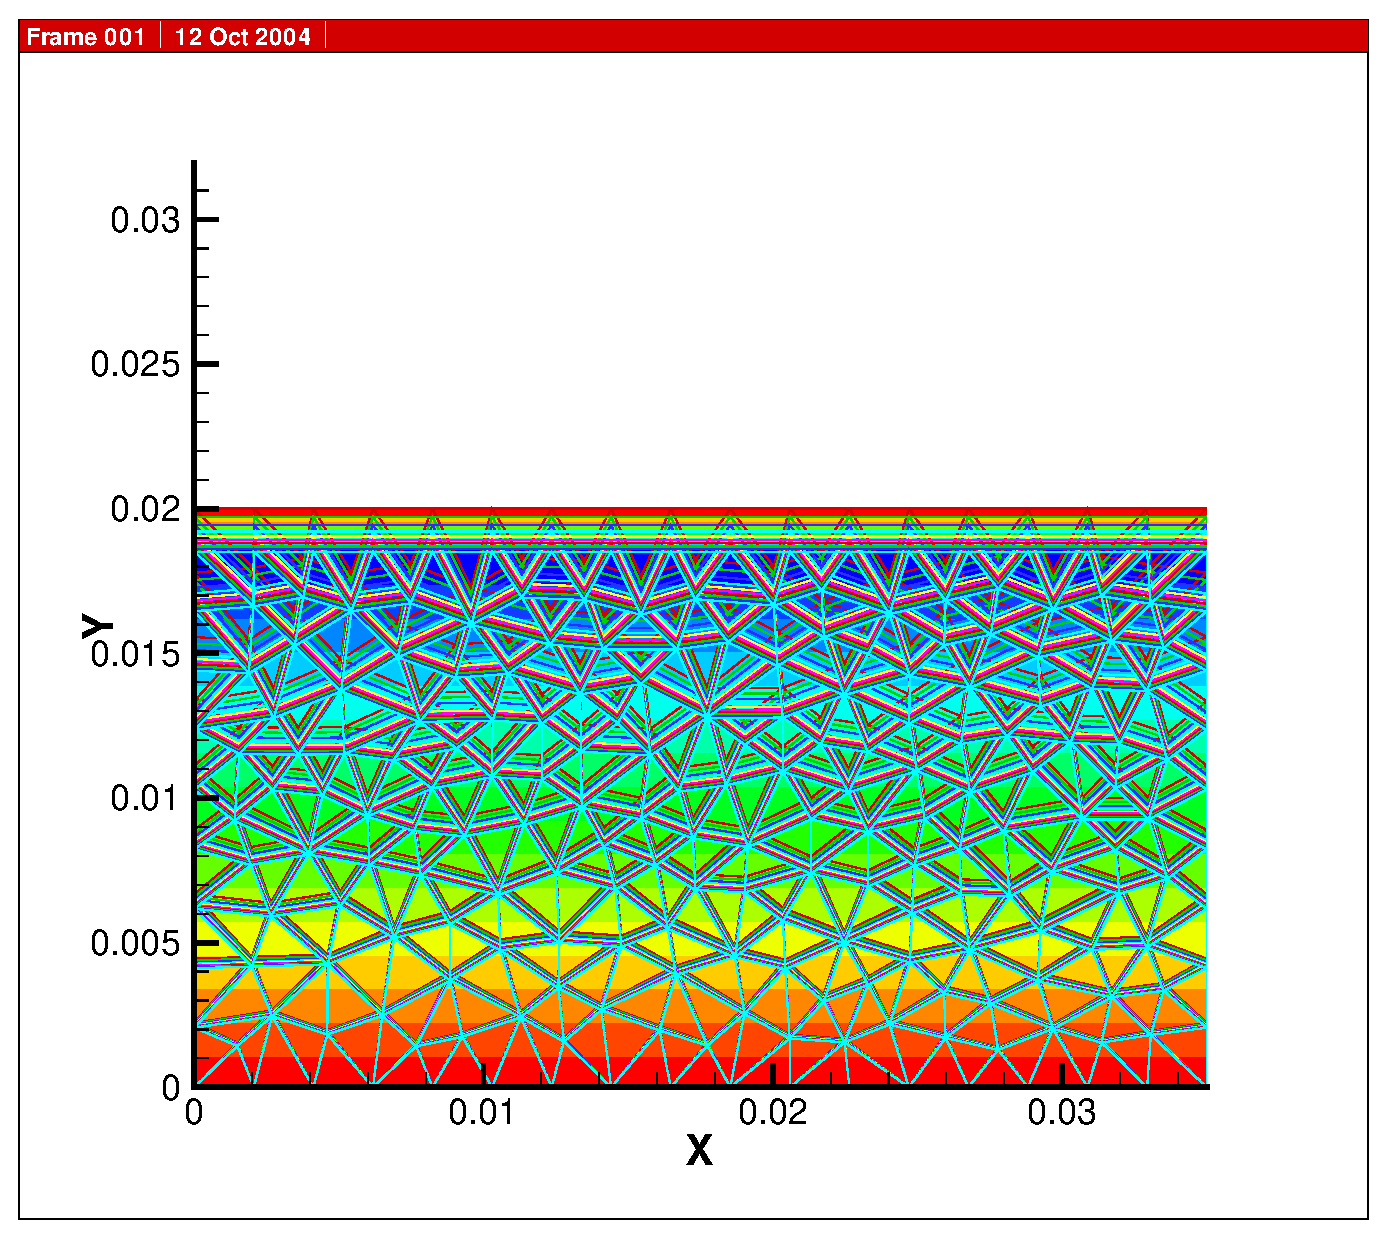
\includegraphics[width=7cm]{figures/m_cc_tri.eps}\\
  %\caption{}\label{}
\end{figure}

\begin{figure}[htb!]
  % Requires \usepackage{graphicx}
  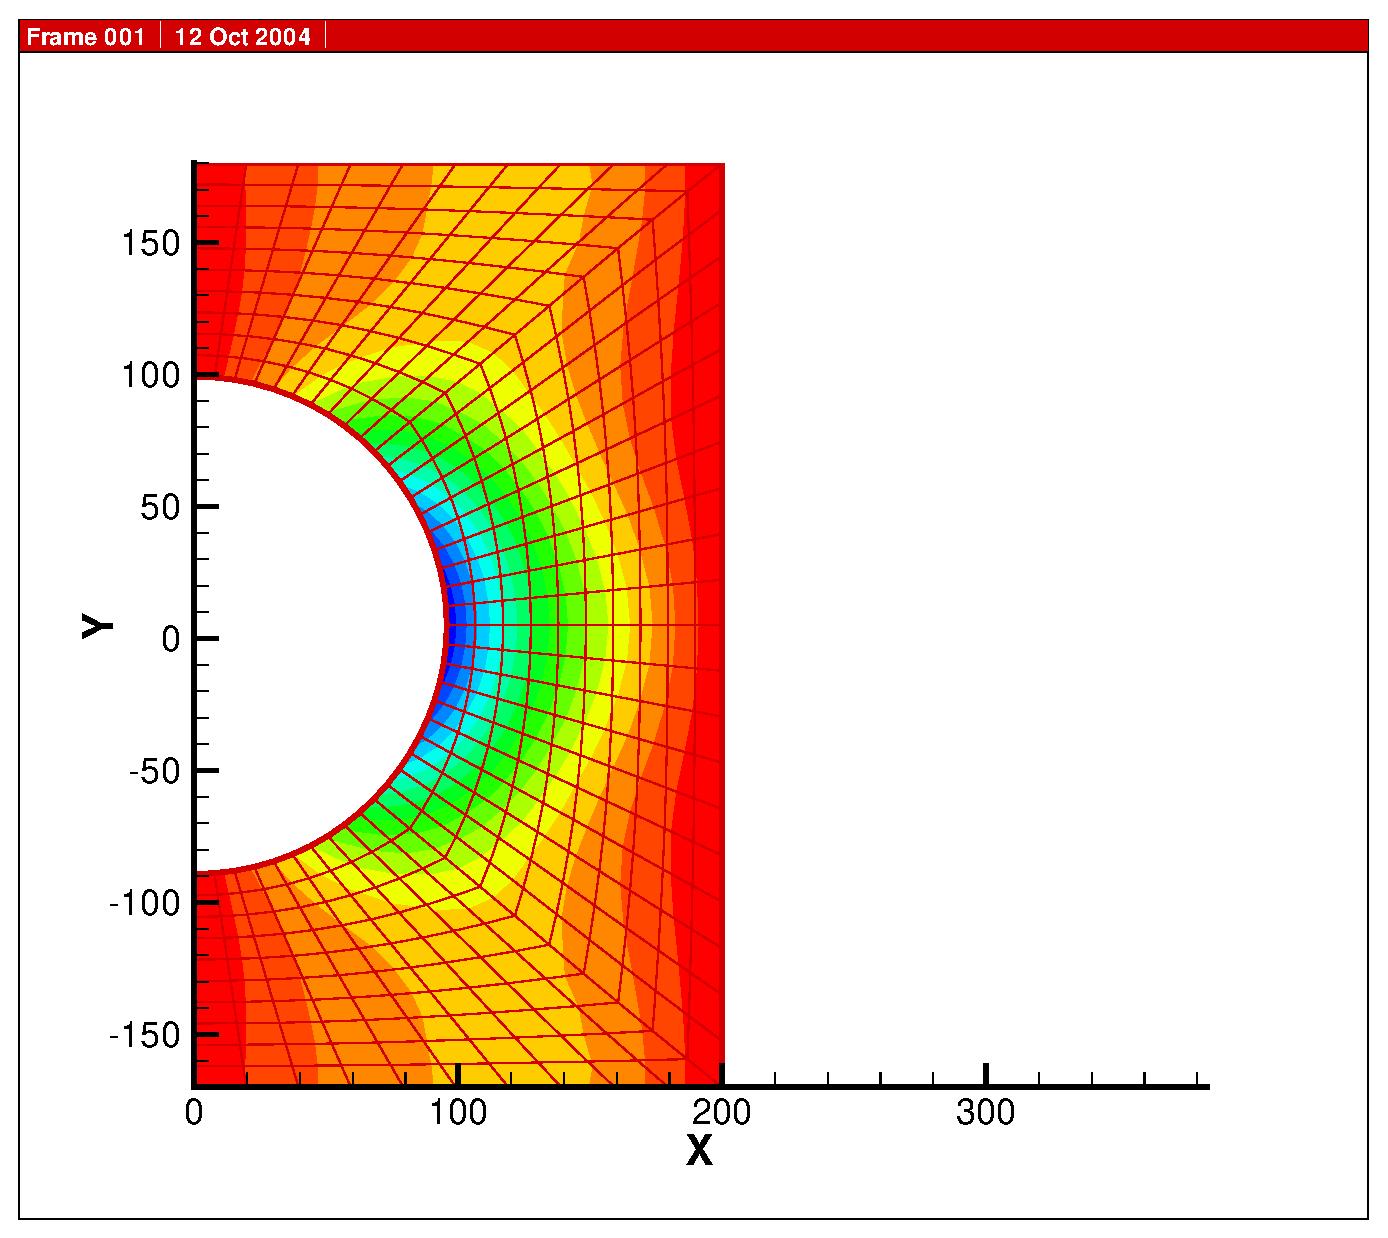
\includegraphics[width=7cm]{figures/m_dp_quad.eps}\\
  %\caption{}\label{}
\end{figure}

\begin{figure}[htb!]
  % Requires \usepackage{graphicx}
  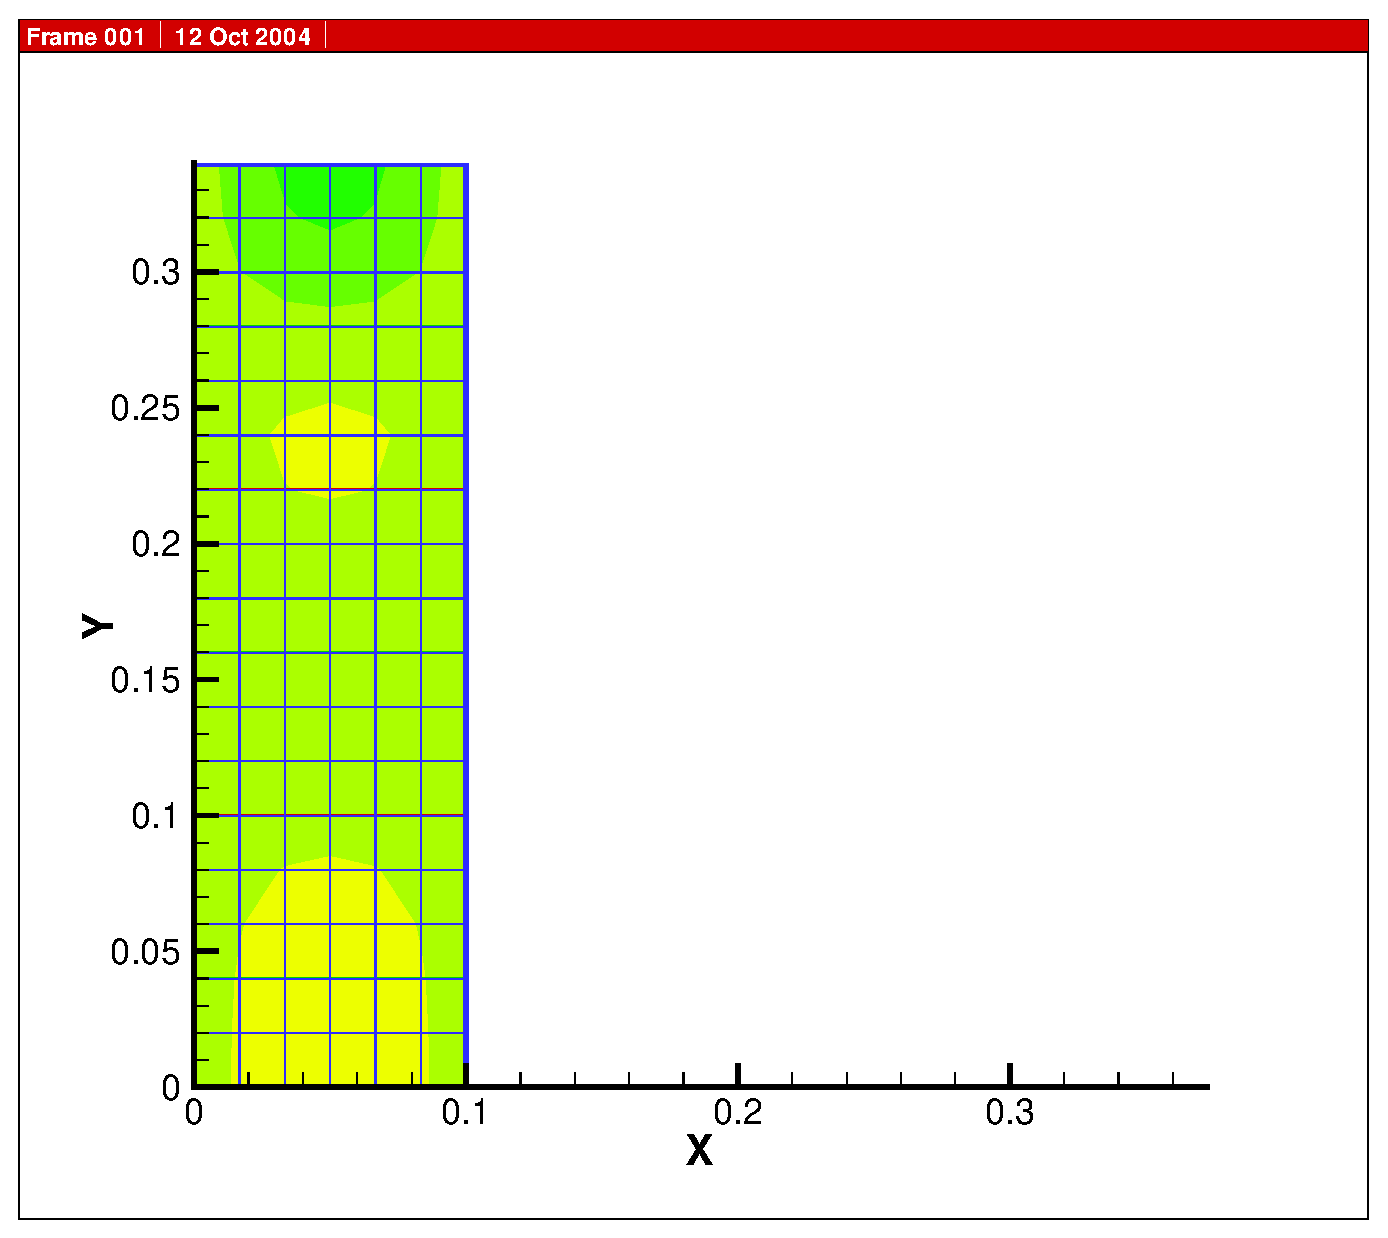
\includegraphics[width=7cm]{figures/m_sys_quad.eps}\\
  %\caption{}\label{}
\end{figure}

\begin{figure}[htb!]
  % Requires \usepackage{graphicx}
  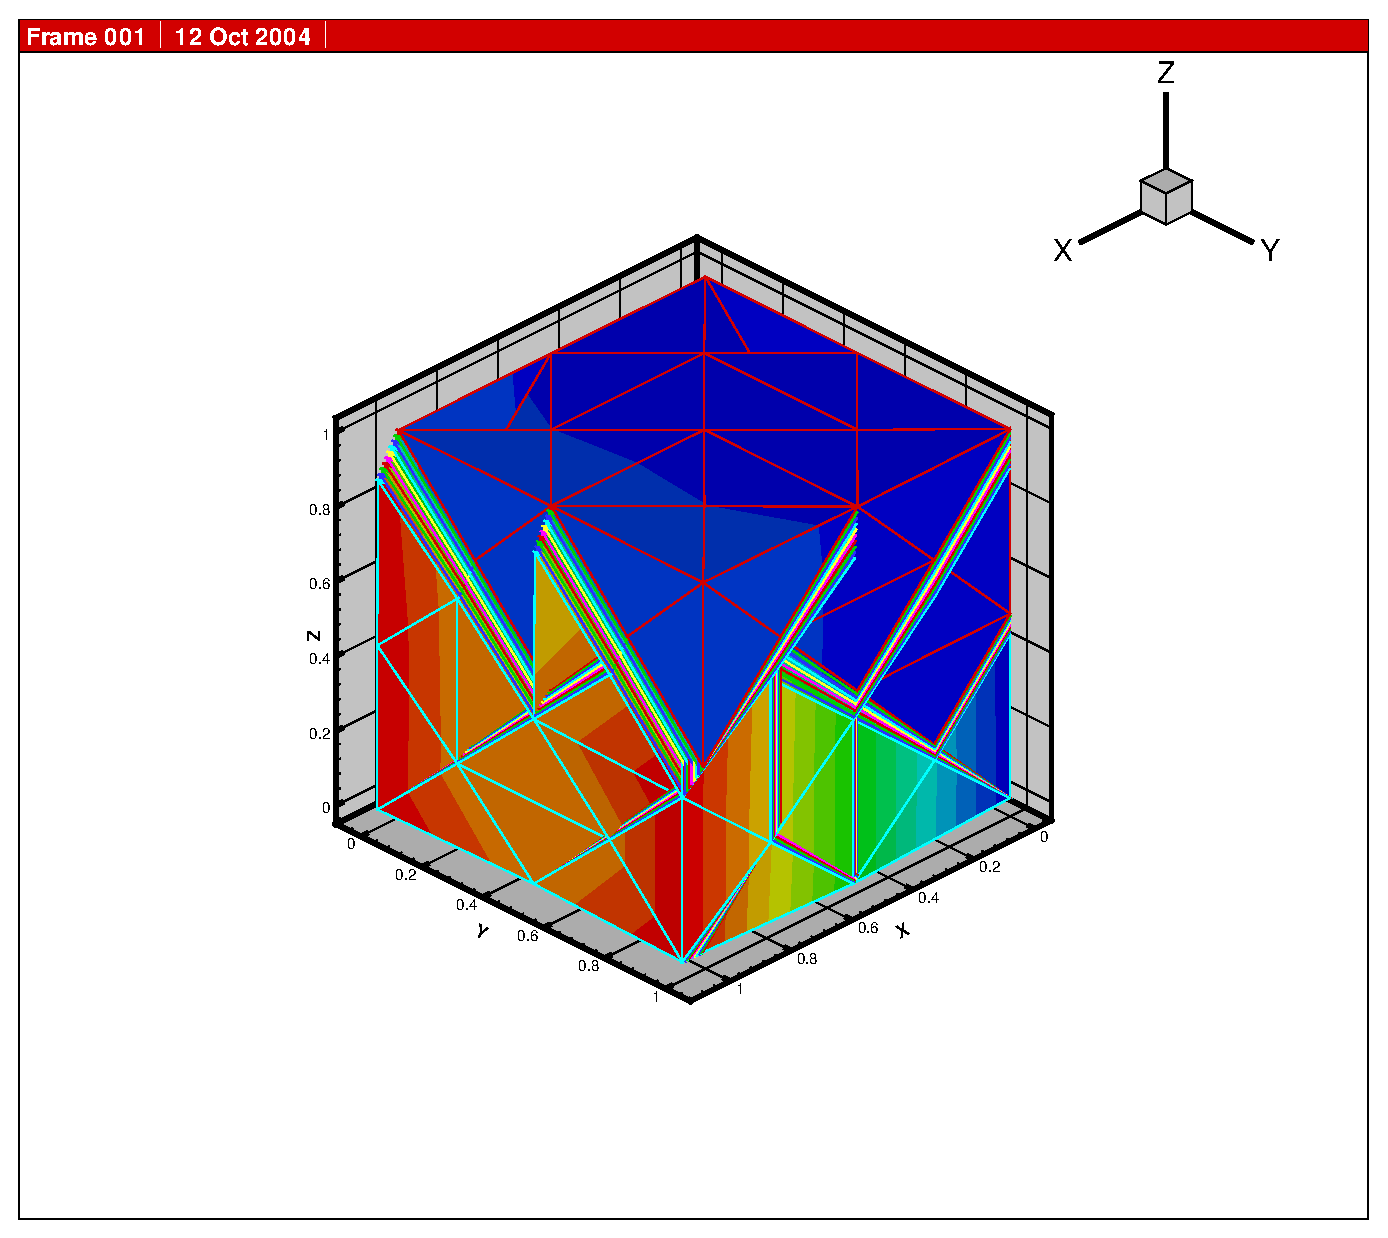
\includegraphics[width=7cm]{figures/m_brick.eps}\\
  %\caption{}\label{}
\end{figure}

\begin{figure}[htb!]
  % Requires \usepackage{graphicx}
  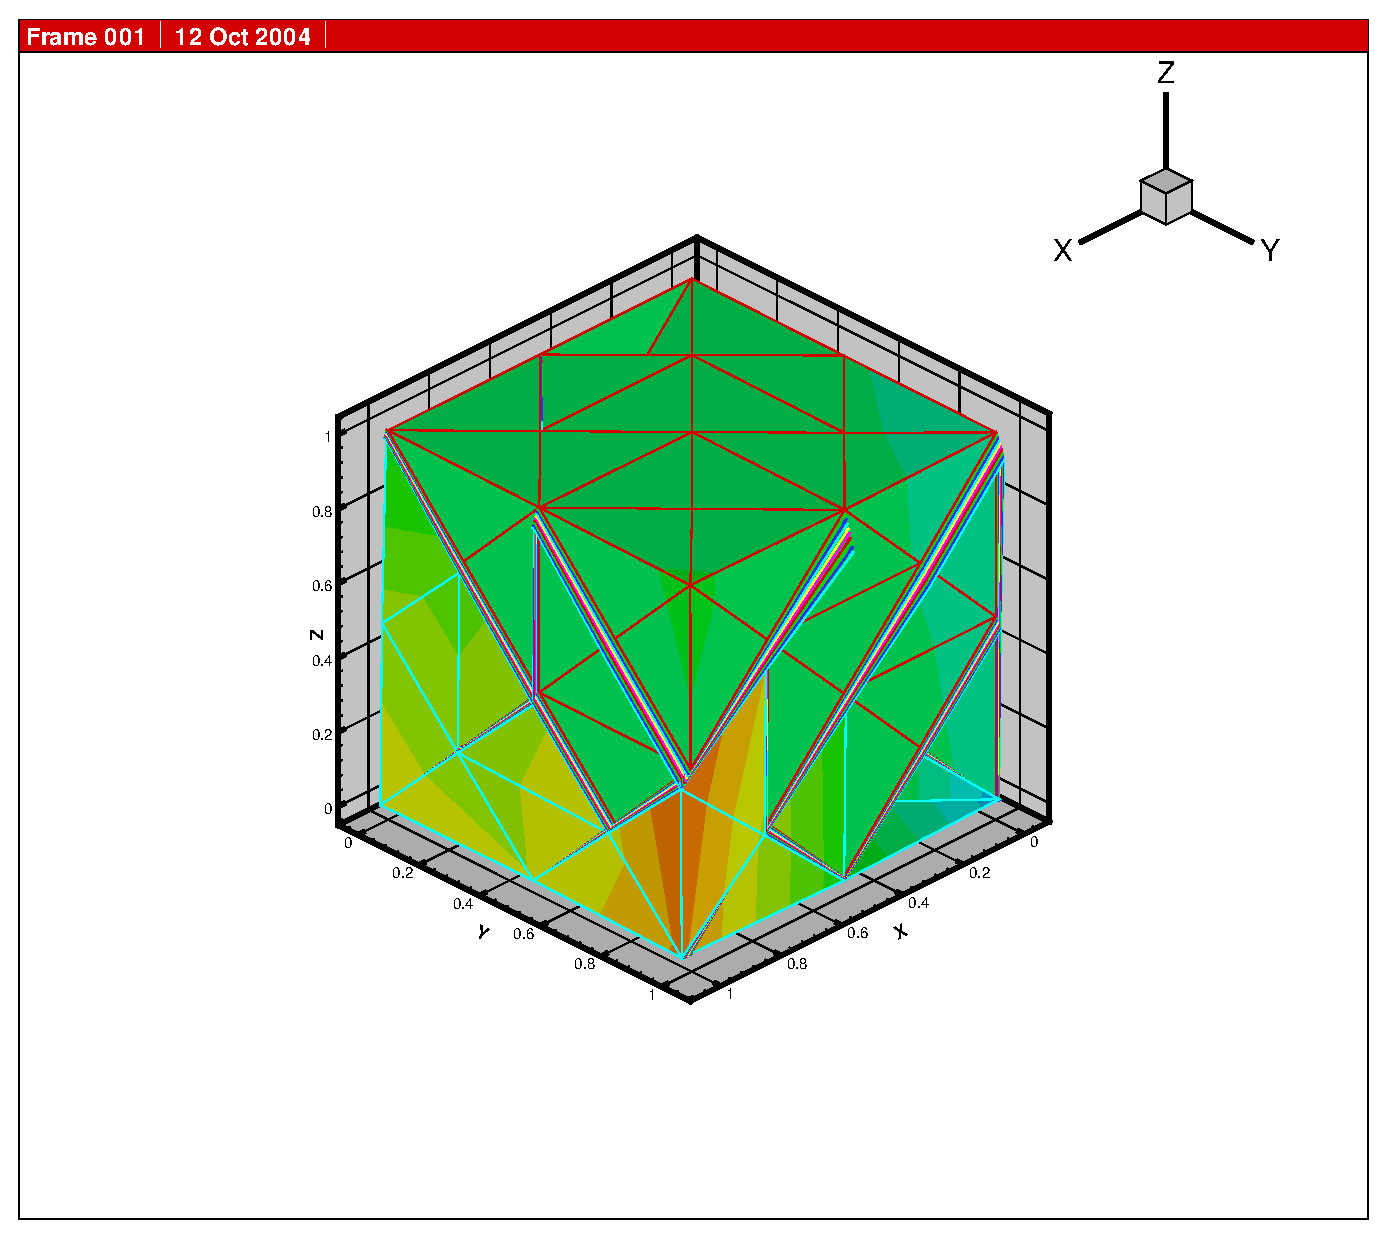
\includegraphics[width=7cm]{figures/m_brick_l.eps}\\
  %\caption{}\label{}
\end{figure}

\newpage $ $ \newpage
\subsection{Consolidation}

\begin{figure}[htb!]
  % Requires \usepackage{graphicx}
  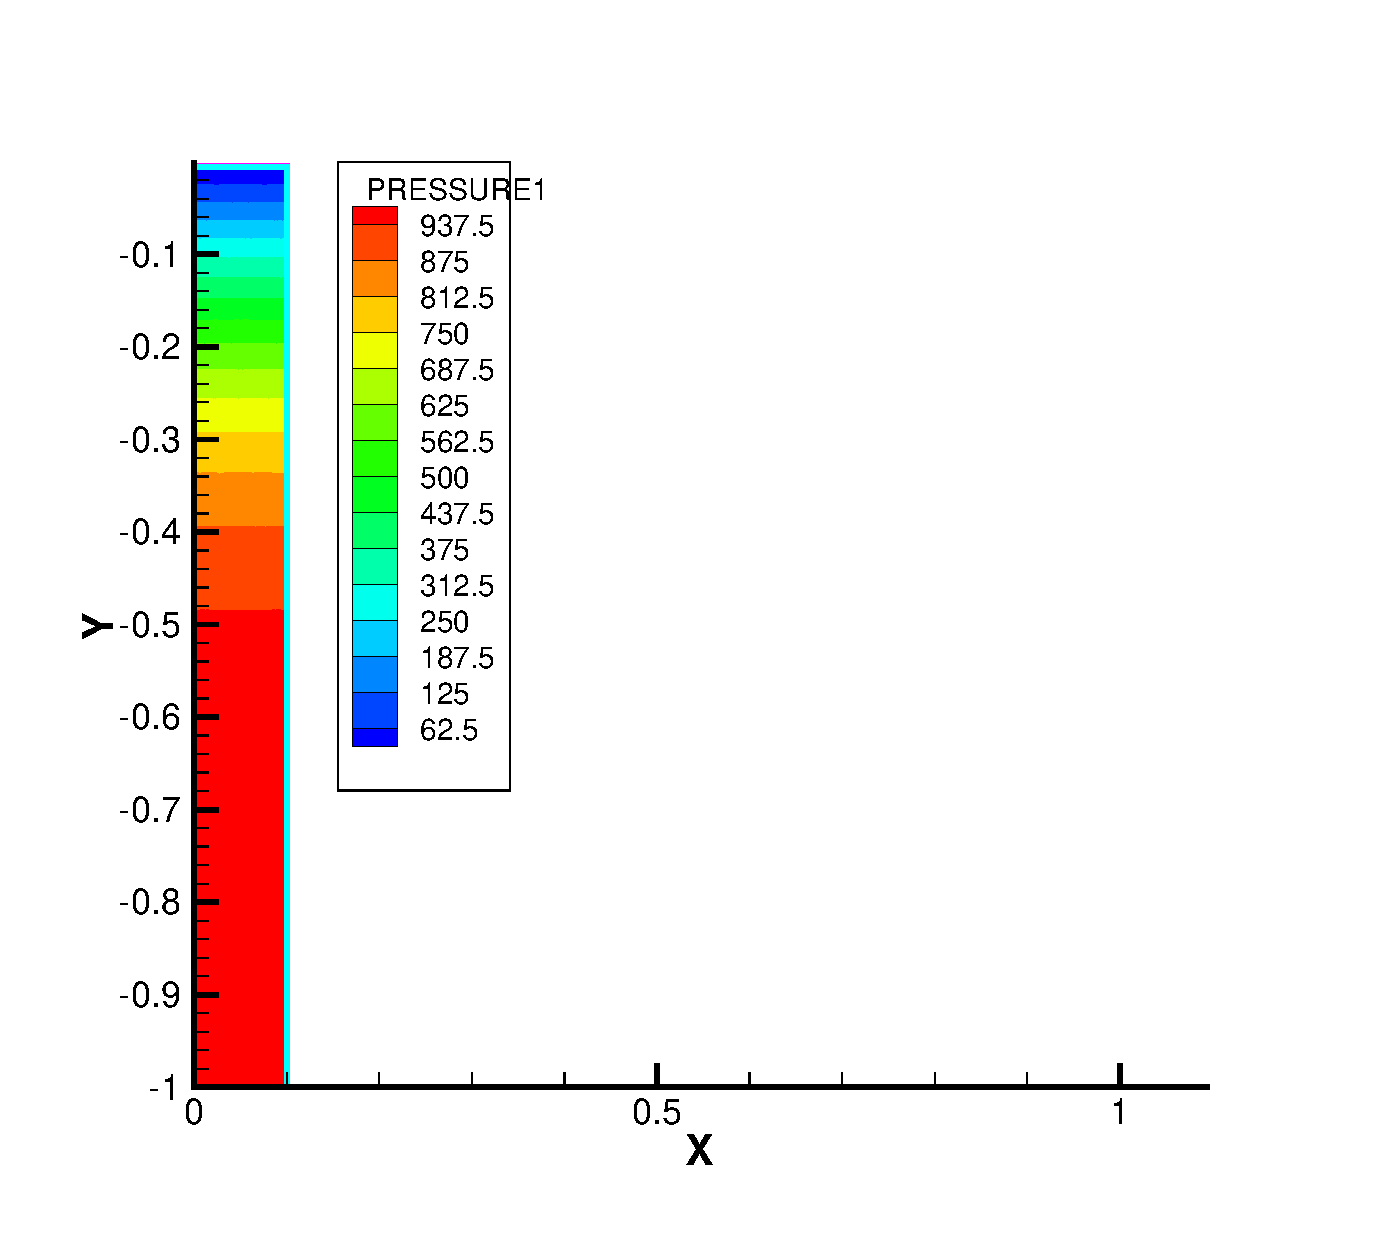
\includegraphics[width=7cm]{figures/hm_tri.eps}\\
  %\caption{}\label{}
\end{figure}

\begin{figure}[htb!]
  % Requires \usepackage{graphicx}
  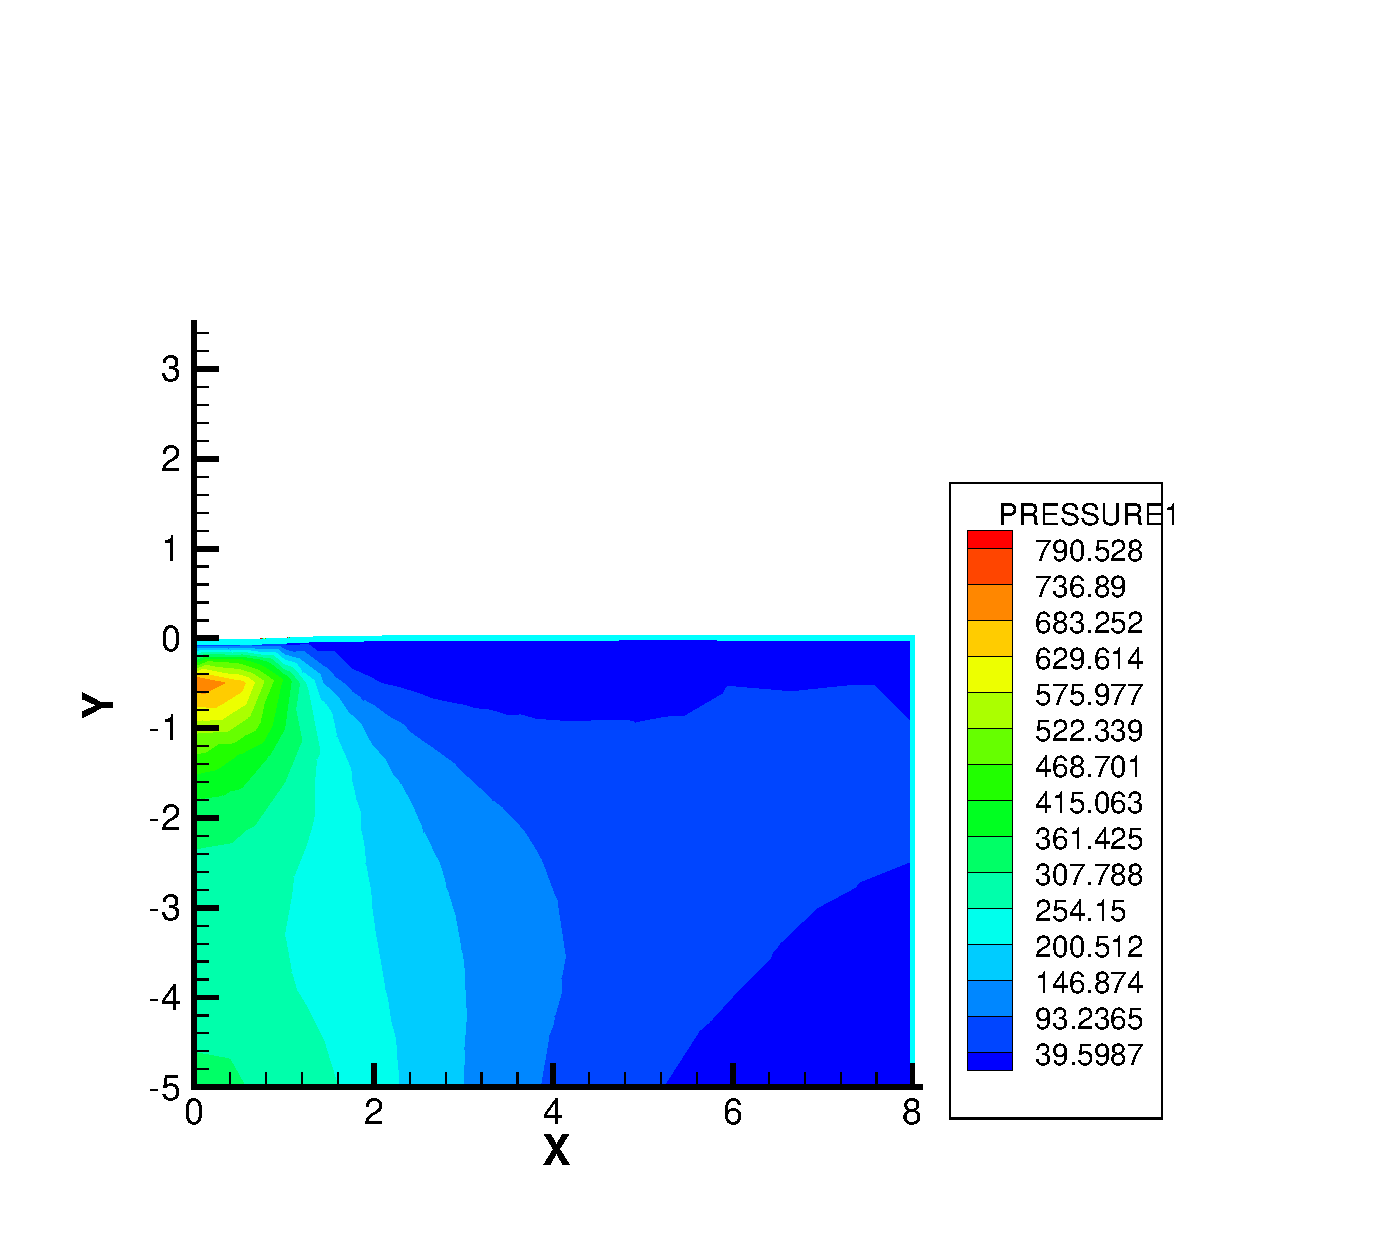
\includegraphics[width=7cm]{figures/hm_foot_tri.eps}\\
  %\caption{}\label{}
\end{figure}

\newpage
\subsection{THM}

\begin{figure}[htb!]
  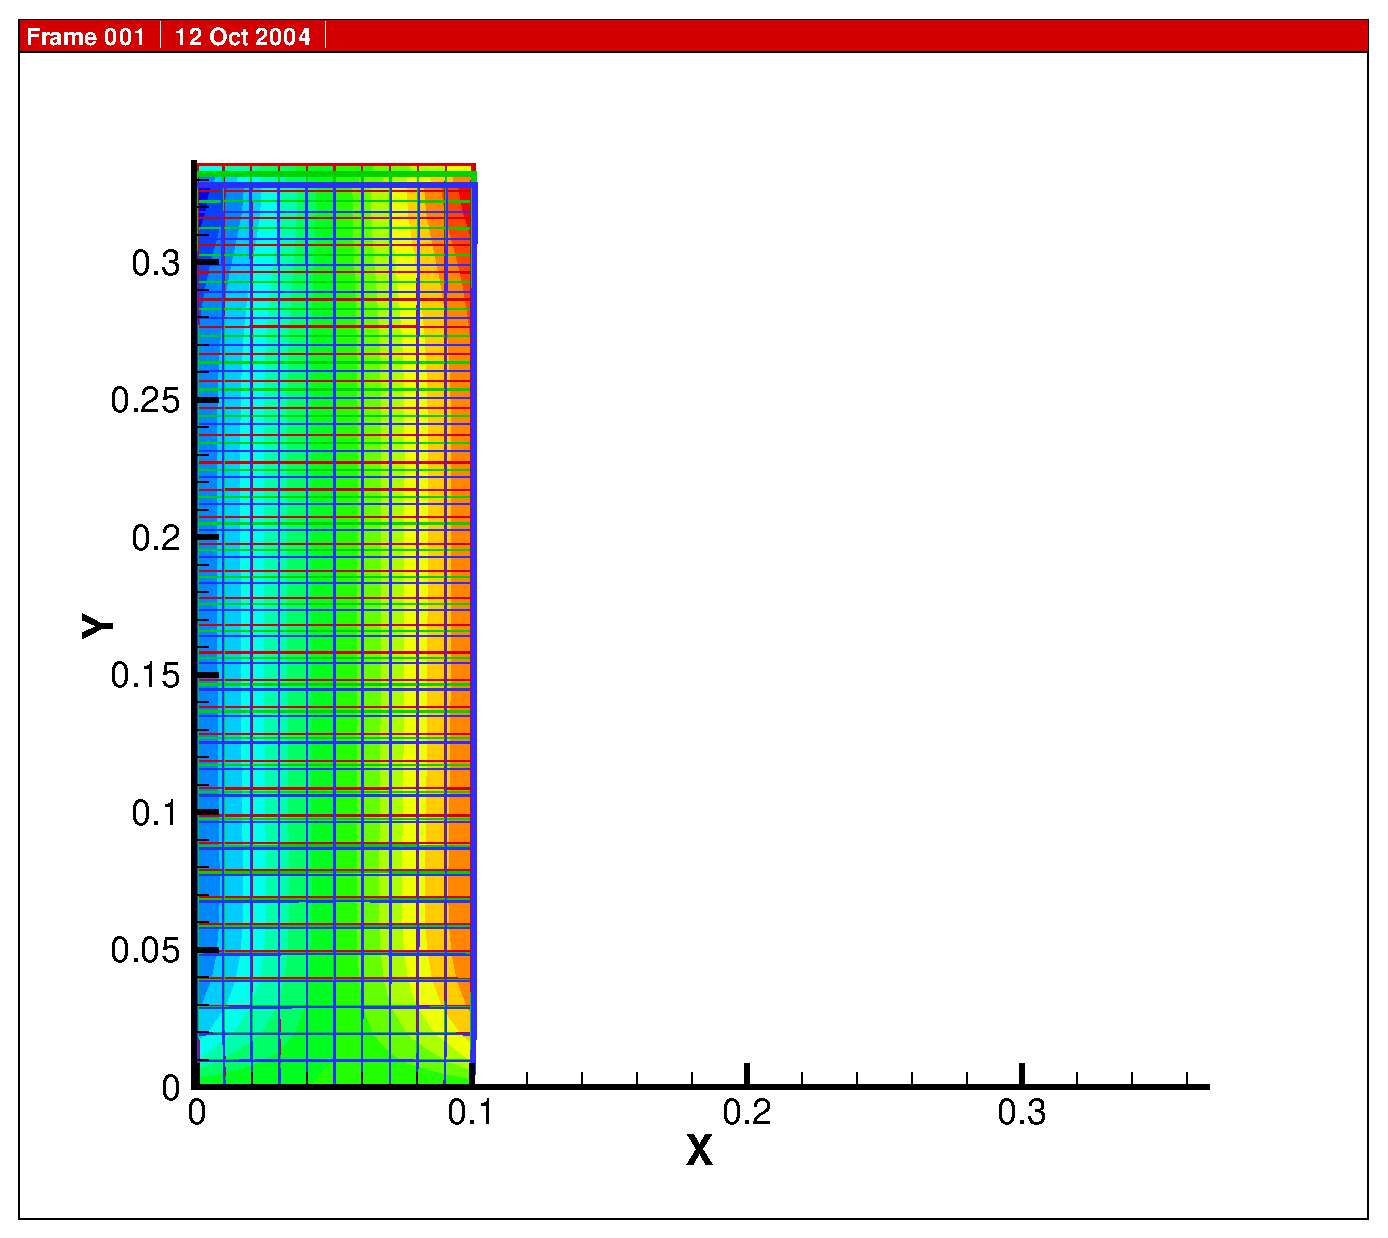
\includegraphics[width=7cm]{figures/thm_quad.eps}\\
\end{figure}

\LastModified{WW - 15th Feb 2006}}

%------------------------------------------
% ToDo list
%%\section{Remarks}

\subsection{V4.1.**MX}

Based on the current version, the following points are to be
considered in the further developments of FEM:

1. Time steps: For reactive transport, different time steps are
needed for different processes. The realized function for that in
the current version is valid for TH2C coupled processes. But for
more processes, a more robust method should be developed in time
class.

2. Various initial conditions for different material groups: This
is the problem of DECOVALEX. For THC simulation,
$\$Material\_DOMAIN$ is used. This can be used only if the mesh is
already generated in *.rfi. This should be in a general way
according to mesh type like $SURFACE$ for 2D.

3. Reaction class: there are two classes (REACT and
REACTION\_MODEL) for reaction. Join them into one?

\subsection{V4.1.13OK}
\subsection{V4.2.04WW}
Gravity orientation is automatically determined by the coordinates 
given  in mesh file as: 
\begin{itemize}
  \item 1D: Only $x$ component has non-zero number $\longrightarrow x$  direction, e.g.,   
           \begin{itemize}
            \item   [x1] 0.0 0.0
            \item   [x2] 0.0 0.0   
            \item  $\vdots$
           \end{itemize}
              
  \item 1D:  Only $z$ component has non-zero number $\longrightarrow z$  direction, e.g.,  
            \begin{itemize}
            \item   0.0 0.0 [z1]
            \item   0.0 0.0 [z2]  
            \item  $\vdots$
           \end{itemize}
  \item 2D:  Gravity in $z$ orientation if $x$ and $z$ components has non-zero number,  
            \begin{itemize}
            \item  [x1] 0.0 [z1]
            \item  [x2] 0.0 [z2]  
            \item  $\vdots$
           \end{itemize}
  \item 2D:  Gravity in $y$ orientation if $x$ and $y$ components has non-zero number,  
            \begin{itemize}
            \item  [x1] [y1]  0.0
            \item  [x2] [y2]  0.0 
            \item  $\vdots$
            \end{itemize}

 \item 3D:  Gravity in always in $z$ orientation even if fracture network is involved.  
\end{itemize}




ToDo things
\begin{itemize}
    \item H-Richards - Celia (YD)
    \item H-Richards - Quad (YD)
    \item M (PCS keyword) (WW)
    \item HM (PCS keyword) (WW)
    \item THM
    \item TH2M
\end{itemize}

\LastModified{OK \today}


%===============================================================================
% Anlagen
%\section{Manual Authors}

\begin{center}
%\begin{tabular*}{13cm}|{p{1.cm}|{p{3.cm}|p{3.cm}|p{1.cm}|} \hline
\begin{tabular}{|l|l|l|l|l|l|}
\hline
Section & Title & Object & Author & & Last modified \\
\hline \hline
%
1 & Preface              &     & OK & ZAG &  \\
2 & Data concept         &     & OK & ZAG &  \\
3 & Processes            & PCS & OK & ZAG &  \\
5 & Time                 & TIM & CB & ZAG &  \\
6 & Output               & OUT & OK & ZAG &  \\
7 & Numerics             & NUM & WW & ZAG &  \\
8 & Solver               & SOL & WW & ZAG &  \\
9  & Initial conditions  & IC  & MB & ZAG &  \\
10 & Boundary conditions & BC  & MK & ISEB &  \\
11 & Source terms        & ST  & OK & ZAG &  \\
12 & Fluid properties    & MAT-FP & JdJ & ZAG &  \\
13 & Solid properties    & MAT-SP & MK & ISEB &  \\
14 & Medium properties   & MAT-MP & CD & ZAG &  \\
15 & Component properties & MAT-CP & MX & ZAG &  \\
16 & Grid adaptation      & ADP & RK & ISEB &  \\
17 & Geometry             & GeoObj & TK/SM & ZAG/ISEB &  \\
18 & Meshing              & MshObj & TK/SM & ZAG/ISEB &  \\
\hline
19 & File formats         &     &    & ZAG &  \\
19.1 & RFI-format           & RFI & TK & ZAG &  \\
19.2 & RFR-format           & RFR & OK & ZAG &  \\
19.3 & GLI-format           & RFM & CC/TK & ZAG &  \\
19.4 & SHP-format           & SHP & CC & ZAG &  \\
\hline
20 & DB interfaces        & WebObj & JG & ZAG &  \\
21 & Parallel computing   & ParObj & DK & ZAG &  \\
\hline
\end{tabular}
\end{center}

%\section{RockFlow History}

\subsection*{Version 1}

\begin{list}{}{\setlength{\itemindent}{-.5cm}}
\item Wollrath, J. (1990): Ein Str\"{o}mungs- und Transportmodell f\"{u}r kl\"{u}ftiges Gestein und Untersuchungen
                     zu homogenen Ersatzsystemen.
                     - Bericht Nr.28/1990, Universit\"{a}t Hannover, Institut f\"{u}r Str\"{o}\-mungs\-mechanik, Dissertationsschrift.

\item Kr\"{o}hn, K.-P. (1991): Simulation von Transportvorg\"{a}ngen im kl\"{u}ftigen Gestein mit der Methode der
                     Finiten-Elemente.
                     - Bericht Nr. 29/1991, Institut f\"{u}r Str\"{o}\-mungs\-mechanik und Elektronisches Rechnen im Bauwesen, Universit\"{a}t Hannover, Dissertationsschrift.
\end{list}


\subsection*{Version 2}


\begin{list}{}{\setlength{\itemindent}{-.5cm}}
\item Helmig, R. (1993): Theorie und Numerik der Mehrphasenstr\"{o}mungen in gekl\"{u}ftet-por\"{o}sen Medien.
  - Dissertationsschrift, Bericht Nr. 34/1993, Institut f\"{u}r Str\"{o}\-mungs\-mechanik, Universit\"{a}t Hannover.

\item Shao, H. (1994): Simulation von Str\"{o}mungs- und Transportvorg\"{a}ngen in gekl\"{u}ftet por\"{o}sen Medien mit
  gekoppelten Finite-Elemente- und Rand-Element-Methoden.
  - Dissertationsschrift, Bericht Nr. 37/1994, Institut f\"{u}r Str\"{o}\-mungs\-mechanik, Universit\"{a}t Hannover.

\item Lege, T. (1995): Modellierung des Kluftgesteins als geologische Barriere f\"{u}r Deponien.
  - Dissertationsschrift,  Institut f\"{u}r Str\"{o}\-mungs\-mechanik und elektronisches Rechnen im Bauwesen, Universit\"{a}t Hannover, 213S.

\item Ratke, R. \& Kolditz, O. \& Zielke, W.  (1996a,b): ROCKFLOW-DM2 - 3-D Dichte\-str\"{o}\-mungsmodell.
  - Technischer Bericht, Institut f\"{u}r Str\"{o}\-mungs\-mechanik und Elektronisches Rechnen im Bauwesen, Universit\"{a}t Han-nover.

\item Kolditz, O. (1996): Stoff- und W\"{a}rmetransport im Kluftgestein. - Habi\-litations\-schrift,
  Institut f\"{u}r Str\"{o}\-mungs\-mechanik und Elektronisches Rechnen im Bauwesen, Universit\"{a}t Hannover, 392S.

\item Barlag C. (1997): Adaptive Methoden zur Modellierung von Stofftransport im Kluftgestein.
  - Dissertationsschrift, Institut f\"{u}r Str\"{o}\-mungs\-mechanik, Universit\"{a}t Hannover.
\end{list}


\subsection*{Version 3}


\begin{list}{}{\setlength{\itemindent}{-.5cm}}
\item Kolditz O., Kaiser R., Thorenz C. \& Schulze-Ruhfus M.: ROCKFLOW User's Manual Release 3.1,
  June 1997, Institut f\"{u}r Str\"{o}\-mungs\-mechanik und Elektronisches Rechnen im Bauwesen, Universit\"{a}t Han-nover.

\item Kolditz O., Habbar A., Kaiser R., Thorenz C.: ROCKFLOW User's Manual Release 3.2,
  December 1997, Institut f\"{u}r Str\"{o}\-mungs\-mechanik und Elektronisches Rechnen im Bauwesen, Universit\"{a}t Hannover.

\item Kolditz O., Habbar A., Kaiser R., Thorenz C.: ROCKFLOW User's Manual Release 3.3,
  November 1998, Institut f\"{u}r Str\"{o}\-mungs\-mechanik und Elektronisches Rechnen im Bauwesen, Universit\"{a}t Hannover.

\item Kolditz O., Habbar A., Kaiser R., Thorenz C.: ROCKFLOW User's Manual Release 3.4,
  November 1999, Institut f\"{u}r Str\"{o}\-mungs\-mechanik und Elektronisches Rechnen im Bauwesen, Universit\"{a}t Hannover.

\item Thorenz, C.: Model Adaptive Simulation of Multiphase and Density Driven Flow in
    Fractured and Porous Media. Dissertation, Institut f\"{u}r Str\"{o}\-mungs\-mechanik, Universit\"{a}t
    Hannover, Bericht Nr. 62/2001.

\item Kaiser, R.: Gitteradaption f\"{u}r die Finite-Elemente-Modellierung gekoppelter Prozesse in
    gekl\"{u}ftet-por\"{o}sen Medien. Dissertation, Institut f\"{u}r Str\"{o}\-mungs\-mechanik, Universit\"{a}t
    Hannover, Bericht Nr. 63/2001.

\item Rother, T.: Geometric Modelling of Geo-Systems. Dissertation, Institut f\"{u}r
    Str\"{o}\-mungs\-mechanik, Universit\"{a}t Hannover, Bericht Nr. 64/2001.

\item Habbar, A.: Direkte und Inverse Modellierung reaktiver Transportprozesse in kl\"{u}ftig-por\"{o}sen Medien.
  Dissertation, Institut f\"{u}r Str\"{o}\-mungs\-mechanik, Universit\"{a}t Hannover, Bericht Nr. 65/2001.

\item Kolditz O, de Jonge J, Beinhorn M, Xie M, Kalbacher T, Wang W, Bauer S, McDermott Ch,
  Kaiser R, Kohlmeier M: ROCKFLOW User's Manual Release 3.9,
  December 2003, Center for Applied Geosciences, Geohydrology/Hydroinformatics,
  Institut f\"{u}r Str\"{o}\-mungs\-mechanik und Elektronisches Rechnen im Bauwesen, Universit\"{a}t Hannover.

\item
\end{list}

\subsection*{Version 4}

{\bf ZAG, T\"{u}bingen:}
\begin{list}{}{\setlength{\itemindent}{-.5cm}}
\item  Olaf Kolditz \\ Computational mechanics, software engineering
\item  Jo\"elle de Jonge \\ Non-isothermal multi-phase /
multi-componental flow
\item  Martin Beinhorn \\ Density-dependent flow with free surfaces
\item  Thomas Kalbacher \\ Geometric modelling, CAD interfaces
\item  Mingliang Xie \\ Geochemical processes in multi-phase systems
\item  Wenqing Wang \\ Inelastic deformation processes in unsaturated
systems
\item  Sebastian Bauer \\ Biogeochemical processes in multi-phase systems
\item  Christopher McDermott \\ GeoEngineering
\item  Cui Chen \\ GIS interface, graphical user interfaces
\item  Jan Gronewold \\ Data bank interfaces, internet information
systems
\item  Christof Beyer \\ Biogeochemical processes, internet information
systems
\item  Dany Kemmler \\ Parallel computing
\item  Dmitro Legeida \\ Dynamic deformation
\item  Andry Ramandriatosoa \\ Geothermal modeling
\item  Robert Walsh \\ Geothermal modeling
\item  Yangliang Du \\ Surface water
\end{list}

{\bf ISEB, Hannover:}

{\bf BGR, Hannover:}

{\bf Associated activities:}
\begin{list}{}{\setlength{\itemindent}{-.5cm}}
\item  Prof. Taniguchi (Okayama University) \\
    Geometric modelling and mesh generation
\end{list}


\LastModified{OK August 13, 2004}


%===============================================================================
% Verzeichnisse
%% Inhaltsverzeichnis
%\newpage
%\tableofcontents
%% Abbildungsverzeichnis
%\newpage
%\listoffigures
%% Tabellenverzeichnis
%\newpage
%\listoftables

\end{document}


%Zaehler
%\setcounter{page}{65}
%\setcounter{section}{8}
%\setcounter{equation}{213}
%\setcounter{figure}{24}
%\setcounter{table}{9}
